\documentclass{beamer}
\DeclareMathOperator*{\argmax}{arg\,max}
\DeclareMathOperator*{\argmin}{arg\,min}
\mode<presentation>
{
  \usetheme{default}
  \usecolortheme{default}
  \usefonttheme{default}
  \setbeamertemplate{navigation symbols}{}
  \setbeamertemplate{caption}[numbered]
}
\usepackage[english]{babel}
\usepackage[utf8x]{inputenc}
\title[M.S. Dissertation]{Optimization and Heuristics for Cognitive Radio Design}
\author{Bharath Keshavamurthy}
\institute{School of Electrical and Computer Engineering, Purdue University}
\date{22 April, 2020}
\begin{document}
\begin{frame}
  \titlepage
\end{frame}
\begin{frame}{Outline}
  \tableofcontents
  \begin{itemize}
      \item \textcolor{blue}{Motivation}
      \item \textcolor{blue}{Related work}
      \item \textcolor{blue}{Challenges tackled in our work}
      \item \textcolor{blue}{The DARPA SC$2$ radio}
      \item \textcolor{blue}{The spectrum sensing and access sub-problem formulation using POMDPs}
      \item \textcolor{blue}{Implementation feasibility analysis on ESP$32$ radios} 
      \item \textcolor{blue}{Summary}
  \end{itemize}
\end{frame}
\begin{frame}{Motivation}
\begin{itemize}
  \item \textcolor{blue}{Infrastructure demands} induced by next-generation RATs (MTC, WSNs, $\dots$) on the consumer side
  \item \textcolor{blue}{Proliferation of military capabilities} reliant on innovation in the wireless landscape (Drone warfare, WPANs, $\dots$)
  \item Re-thinking \textcolor{blue}{Spectrum Licensing} (FCC-CBRS)
  \item \textcolor{blue}{National Security} interests in communications infrastructure (US-China Huawei 5G)
  \item \textcolor{blue}{Advancements in A.I. and SDRs} (Collaborate v Compete)
\end{itemize}
\end{frame}
\begin{frame}{Related Work}
\begin{itemize}
  \item \scriptsize{The DARPA SC$2$ competitors: Their design principles}
  \begin{itemize}
      \item \scriptsize{\textcolor{blue}{SCATTER}\footnote{\tiny{Giannoulis, et. al., ``The SCATTER approach...", 2019 IEEE DySPAN}}: OFDM waveform, McF-TDMA, Distributed channel allocation, Target-score based flow scheduling}
      \item \scriptsize{\textcolor{blue}{Zylinium}\footnote{\tiny{R.J. Baxley, R.S. Thompson, ``Team Zylinium...", 2019 IEEE DySPAN}}: OFDM PHY, MCS adaptation, Purely CIL based centralized channel allocation, Mixed integer programming for flow scheduling}
  \end{itemize}
  \item \scriptsize{Tackling the spectrum sensing and access problem using MABs\footnote{\label{F5}\tiny{K. Cohen, et. al., ``Restless Multi-Armed Bandits...", 2014 Asilomar}}, RL-agents\footnote{\label{F3}\tiny{J. Lund\'{e}n, et. al., ``Multiagent Spectrum Sensing...", IEEE Journal of Selected Topics in Signal Processing}}, custom heuristics\footnote{\label{F4}\tiny{M. Gao, et. al., ``Fast Spectrum Sensing...", 2014 IEEE MilCom}}: \textcolor{red}{Issues}}
  \begin{itemize}
      \item \scriptsize{\textcolor{red}{Noise-free} [\ref{F4}] observation model or \textcolor{red}{Ignored} [\ref{F3}] errors in state estimation (impractical)}
      \item \scriptsize{\textcolor{red}{Failure to exploit} [\ref{F5}] the incumbent occupancy time-frequency correlation structure (imprudent)}
      \item \scriptsize{\textcolor{red}{Apriori knowledge}\footnote{\label{F6}\tiny{C. Park, et. al., ``HMM Based Channel Status Predictor for Cognitive Radio", 2007 Asia-Pacific Microwave Conference}} of this correlation model (impractical)}
      \item \scriptsize{\textcolor{red}{Offline estimation} [\ref{F4}] of this correlation model (impractical)}
      \item \scriptsize{\textcolor{red}{No support} ([\ref{F3}], [\ref{F4}]) for tuning throughput and interference}
  \end{itemize}
\end{itemize}
\end{frame}
\begin{frame}{Challenges tackled in our work (1/2)}
\begin{itemize}
    \item The DARPA SC$2$ radio: Our design principles
    \begin{itemize}
        \item Value-per-resource \textcolor{blue}{prioritized flow scheduling} with recursive revisitation, deficit round-robin queueing, and ARQ for bursty file transfers
        \item Robust \textcolor{blue}{FSK control channel} (short control frames) \item \textcolor{blue}{DFT-s-OFDM data channel} (traffic interleaved with long control frames)
        \item \textcolor{blue}{MCS adaptation} based on consecutive constellation symbol distance minimization
        \item PSD measurements + Collaboration messages drive \textcolor{blue}{channel allocation}
        \item Link quality + Traffic demands drive \textcolor{blue}{bandwidth allocation}
        \item \textcolor{blue}{Multi-hop routing with Dijkstra's} applied over routing tables shared over the control channel
    \end{itemize}
\end{itemize}
\end{frame}
\begin{frame}{Challenges tackled in our work (2/2)}
\begin{itemize}
    \item The spectrum sensing and access sub-problem\footnote{\tiny{B. Keshavamurthy, N. Michelusi, ``Spectrum Sensing in Cognitive Radio Networks via Approximate POMDP", Unpublished, 2020}}: \textcolor{cyan}{Novelties}
    \begin{itemize}
        \item \textcolor{cyan}{Noisy} observation model with Rayleigh fading channels
        \item \textcolor{cyan}{Successfully exploit} incumbent occupancy time-frequency correlation structure by approximating it with a double Markov chain model
        \item \textcolor{cyan}{No apriori knowledge} of this correlation model
        \item \textcolor{cyan}{Online estimation} of this correlation model
        \item \textcolor{cyan}{Approximate POMDP} for computationally tractable spectrum sensing\texttt{-{}-}with spectrum access decisions driven by MAP state estimation involving the posterior belief
        \item \textcolor{cyan}{Fragmentation} and Belief update simplification using \textcolor{cyan}{Hamming distance filters}
        \item \textcolor{cyan}{Support} for throughput and interference tuning
    \end{itemize}
    \item \textcolor{blue}{Implement} the optimal channel access policy on an ad-hoc distributed network of ESP$32$ radios
\end{itemize}
\end{frame}
\begin{frame}{}
  \centering \Huge
  \emph{The DARPA SC$2$ radio}
\end{frame}
\begin{frame}{Purdue BAM! Wireless CIRN deployment architecture}
\begin{figure}
    \centering
    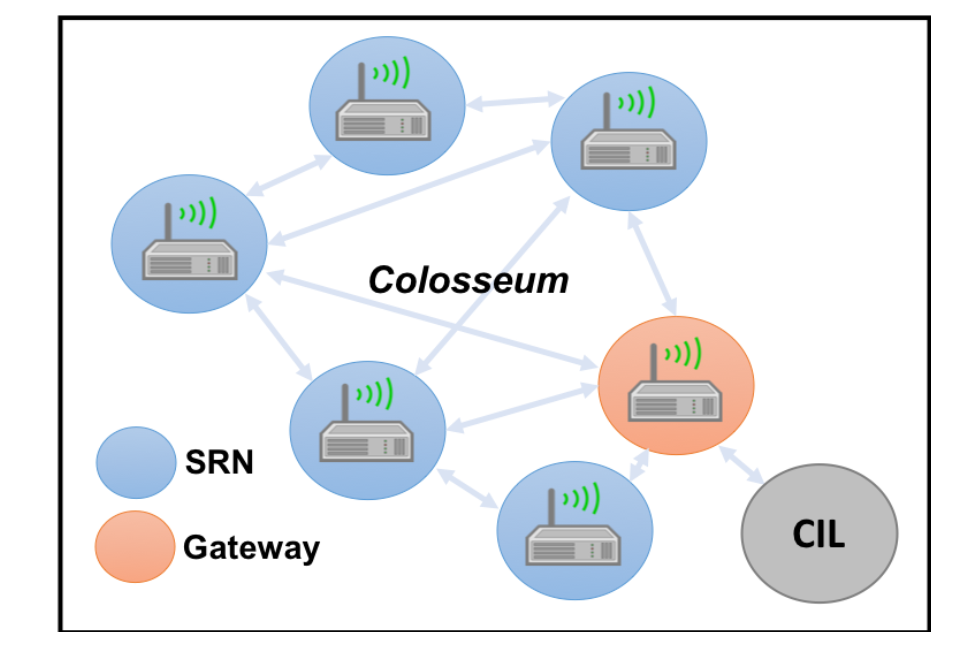
\includegraphics[width = 0.95\textwidth]{BAM!_Wireless_Architecture.PNG}
    \caption{CIRN architecture in any given Colosseum scenario}
    \label{fig:1}
\end{figure}
\end{frame}
\begin{frame}{PHY: Transmission Power Control (1/4)}
    \footnotesize{\begin{itemize}
        \item All competitors should collaborate to ensure incumbent interference compliance
        \item Incumbents governed by pre-determined threshold changes + Violation driven threshold changes
        \item Report and Violation messages from the incumbent
        \item Violation: Aggregate interference at the incumbent exceeds threshold\texttt{-{}-}monitor CIL messages to determine the number of users using the incumbent's bands ($\Lambda$); reduce each node's Tx power as follows
        \item \[P_{T}'=P_{T}-\left(\frac{P_{obs}-\omega P_{th}}{\Lambda}\right);\ P_{obs}=10\log_{10}(I^{2}{+}Q^{2})-31.5\]
        $P_{T}$ denotes the transmit power of SRNs in our network (in dBFS);
        \\$P_{obs}$ denotes the relative-power measured at the Passive Incumbent (in dBFS);
        \\$P_{th}$ denotes the current threshold of the Passive Incumbent (in dBFS);
        \\$\omega$ (slightly less than $1$) is a multiplicative offset factor to account for synchronization inconsistencies
        \item \[P_{obs}=\sum_{\nu}\sum_{\mu}(P_{T}')^{\nu,\mu}=\sum_{\lambda=1}^{\Lambda}\left(P_{T}-\frac{\Lambda P_{T}}{\Lambda}+\frac{{\omega}P_{th}}{\Lambda}\right)={\omega}P_{th}<P_{th}\]
    \end{itemize}}
\end{frame}
\begin{frame}{PHY: Transmission Power Control (2/4)}
\begin{figure}
    \centering
    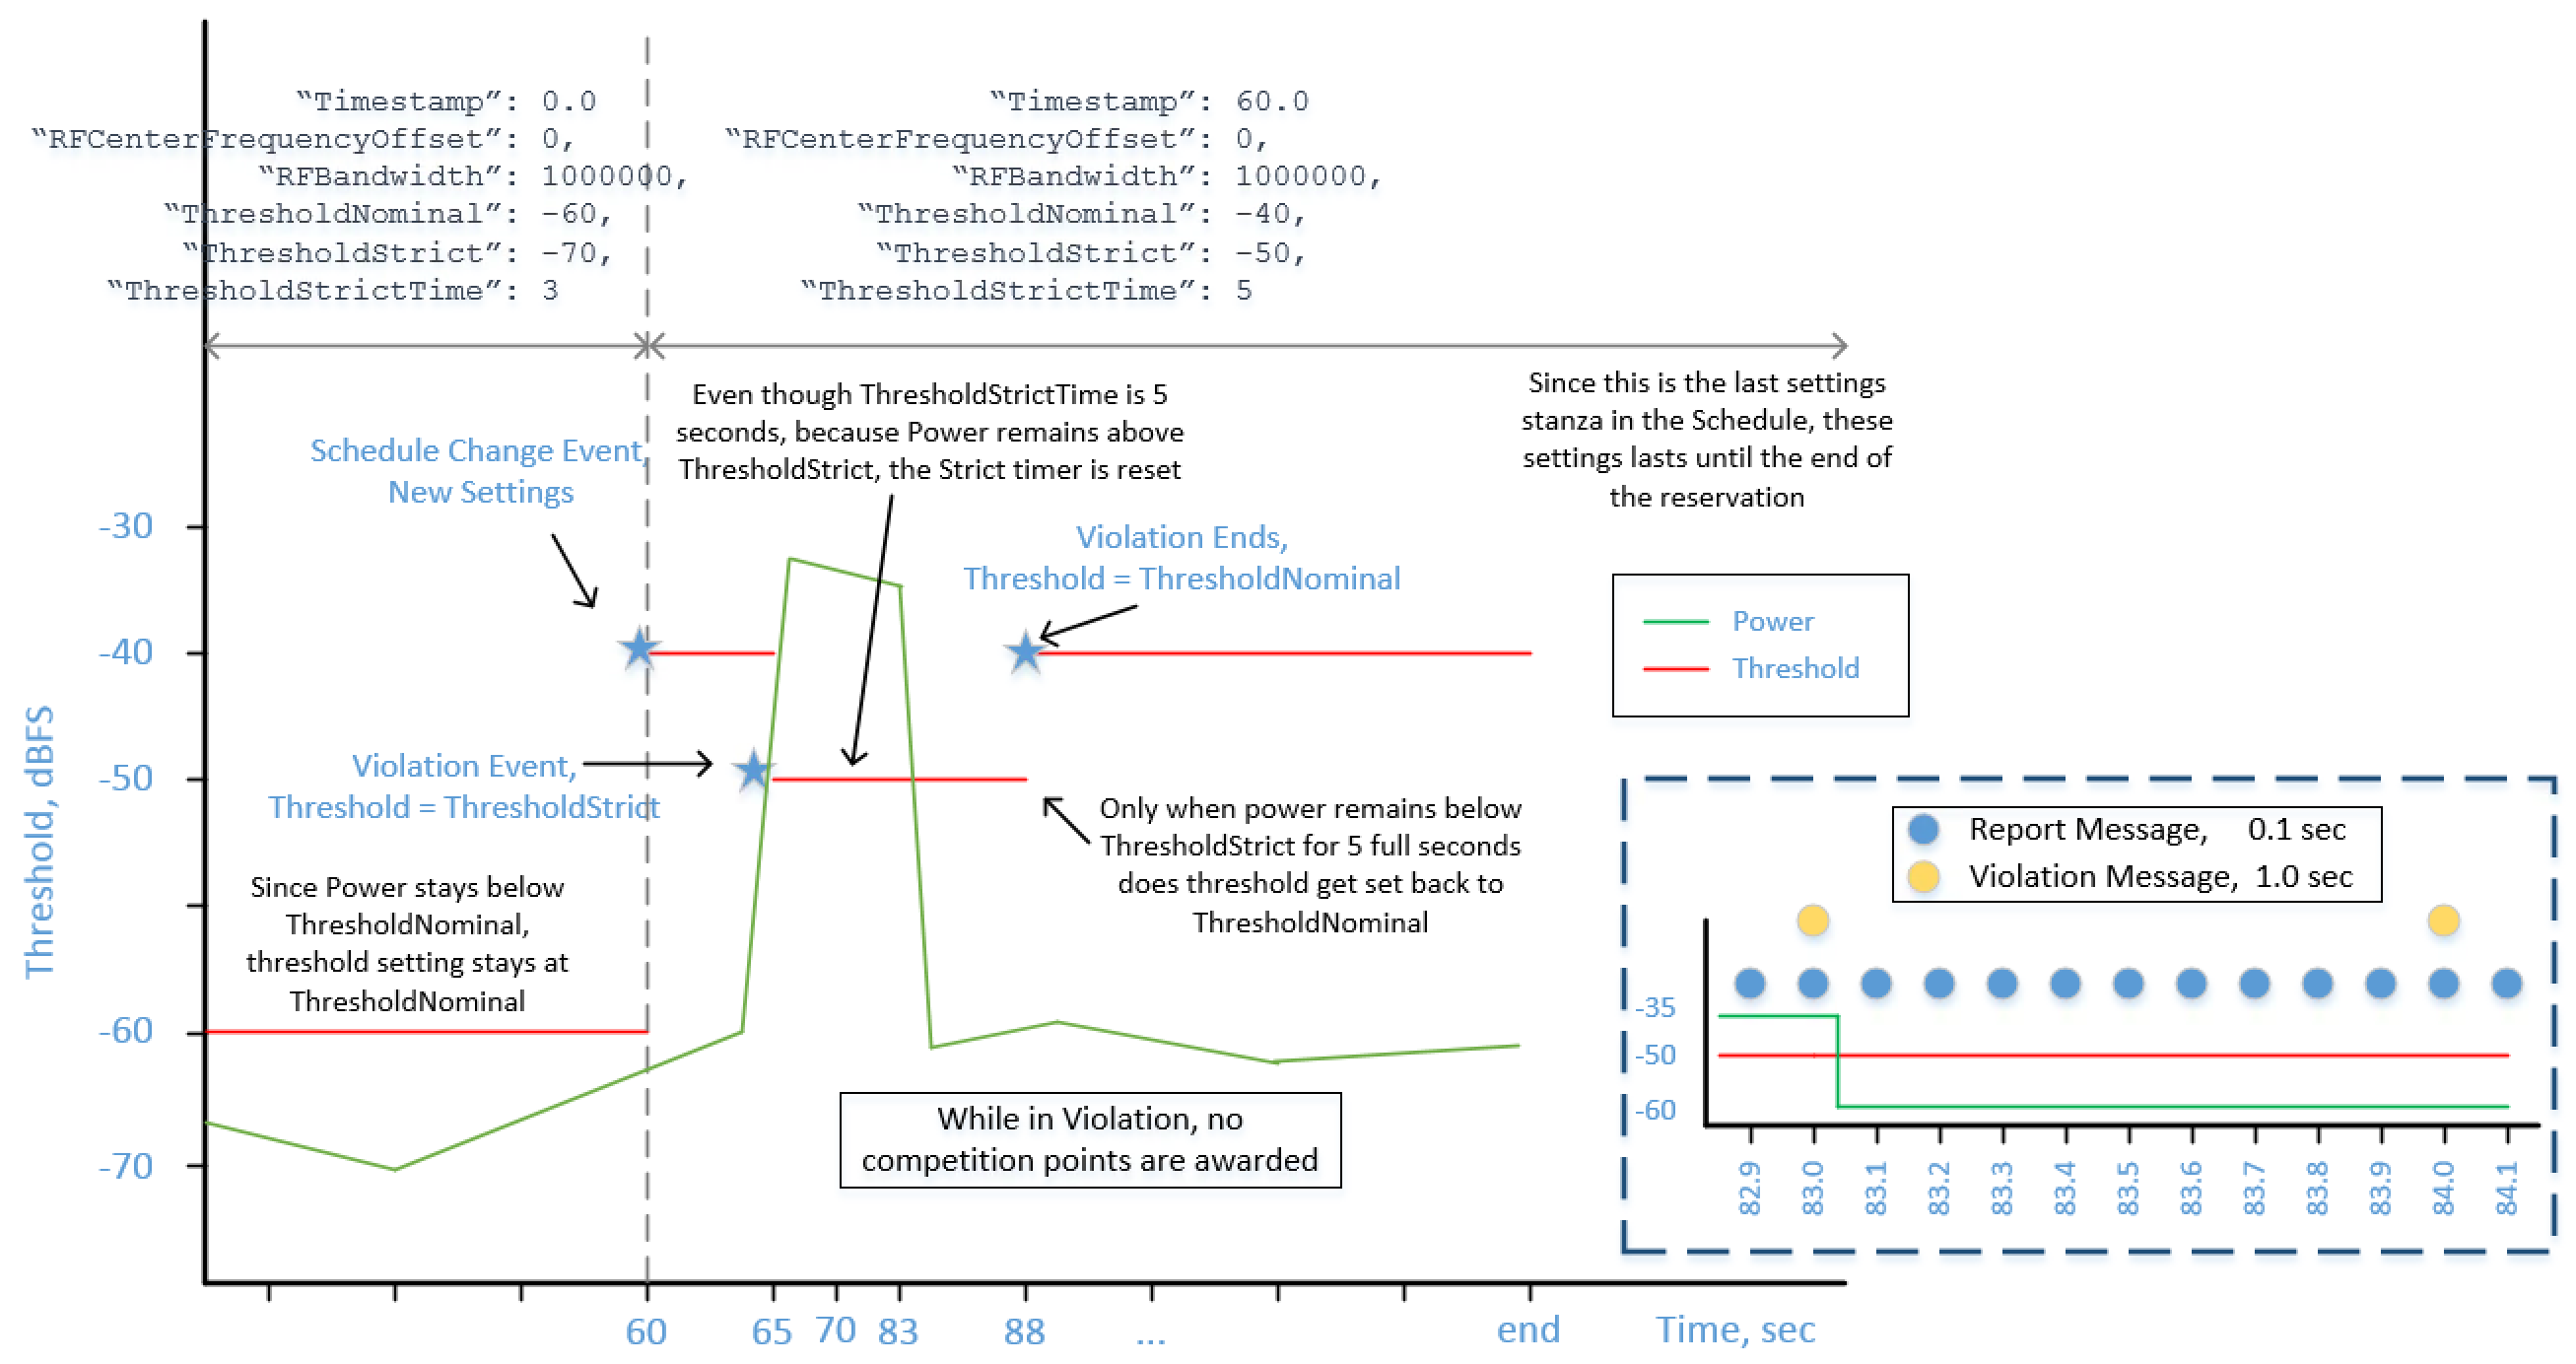
\includegraphics[width = 0.95\textwidth]{Passive_Incumbent.jpg}
    \caption{The temporal behavior of the Passive Incumbent\footnote{\tiny{DARPA Colosseum}}}
    \label{fig:2}
\end{figure}
\end{frame}
\begin{frame}{PHY: Transmission Power Control (3/4)}
\begin{figure}
    \centering
    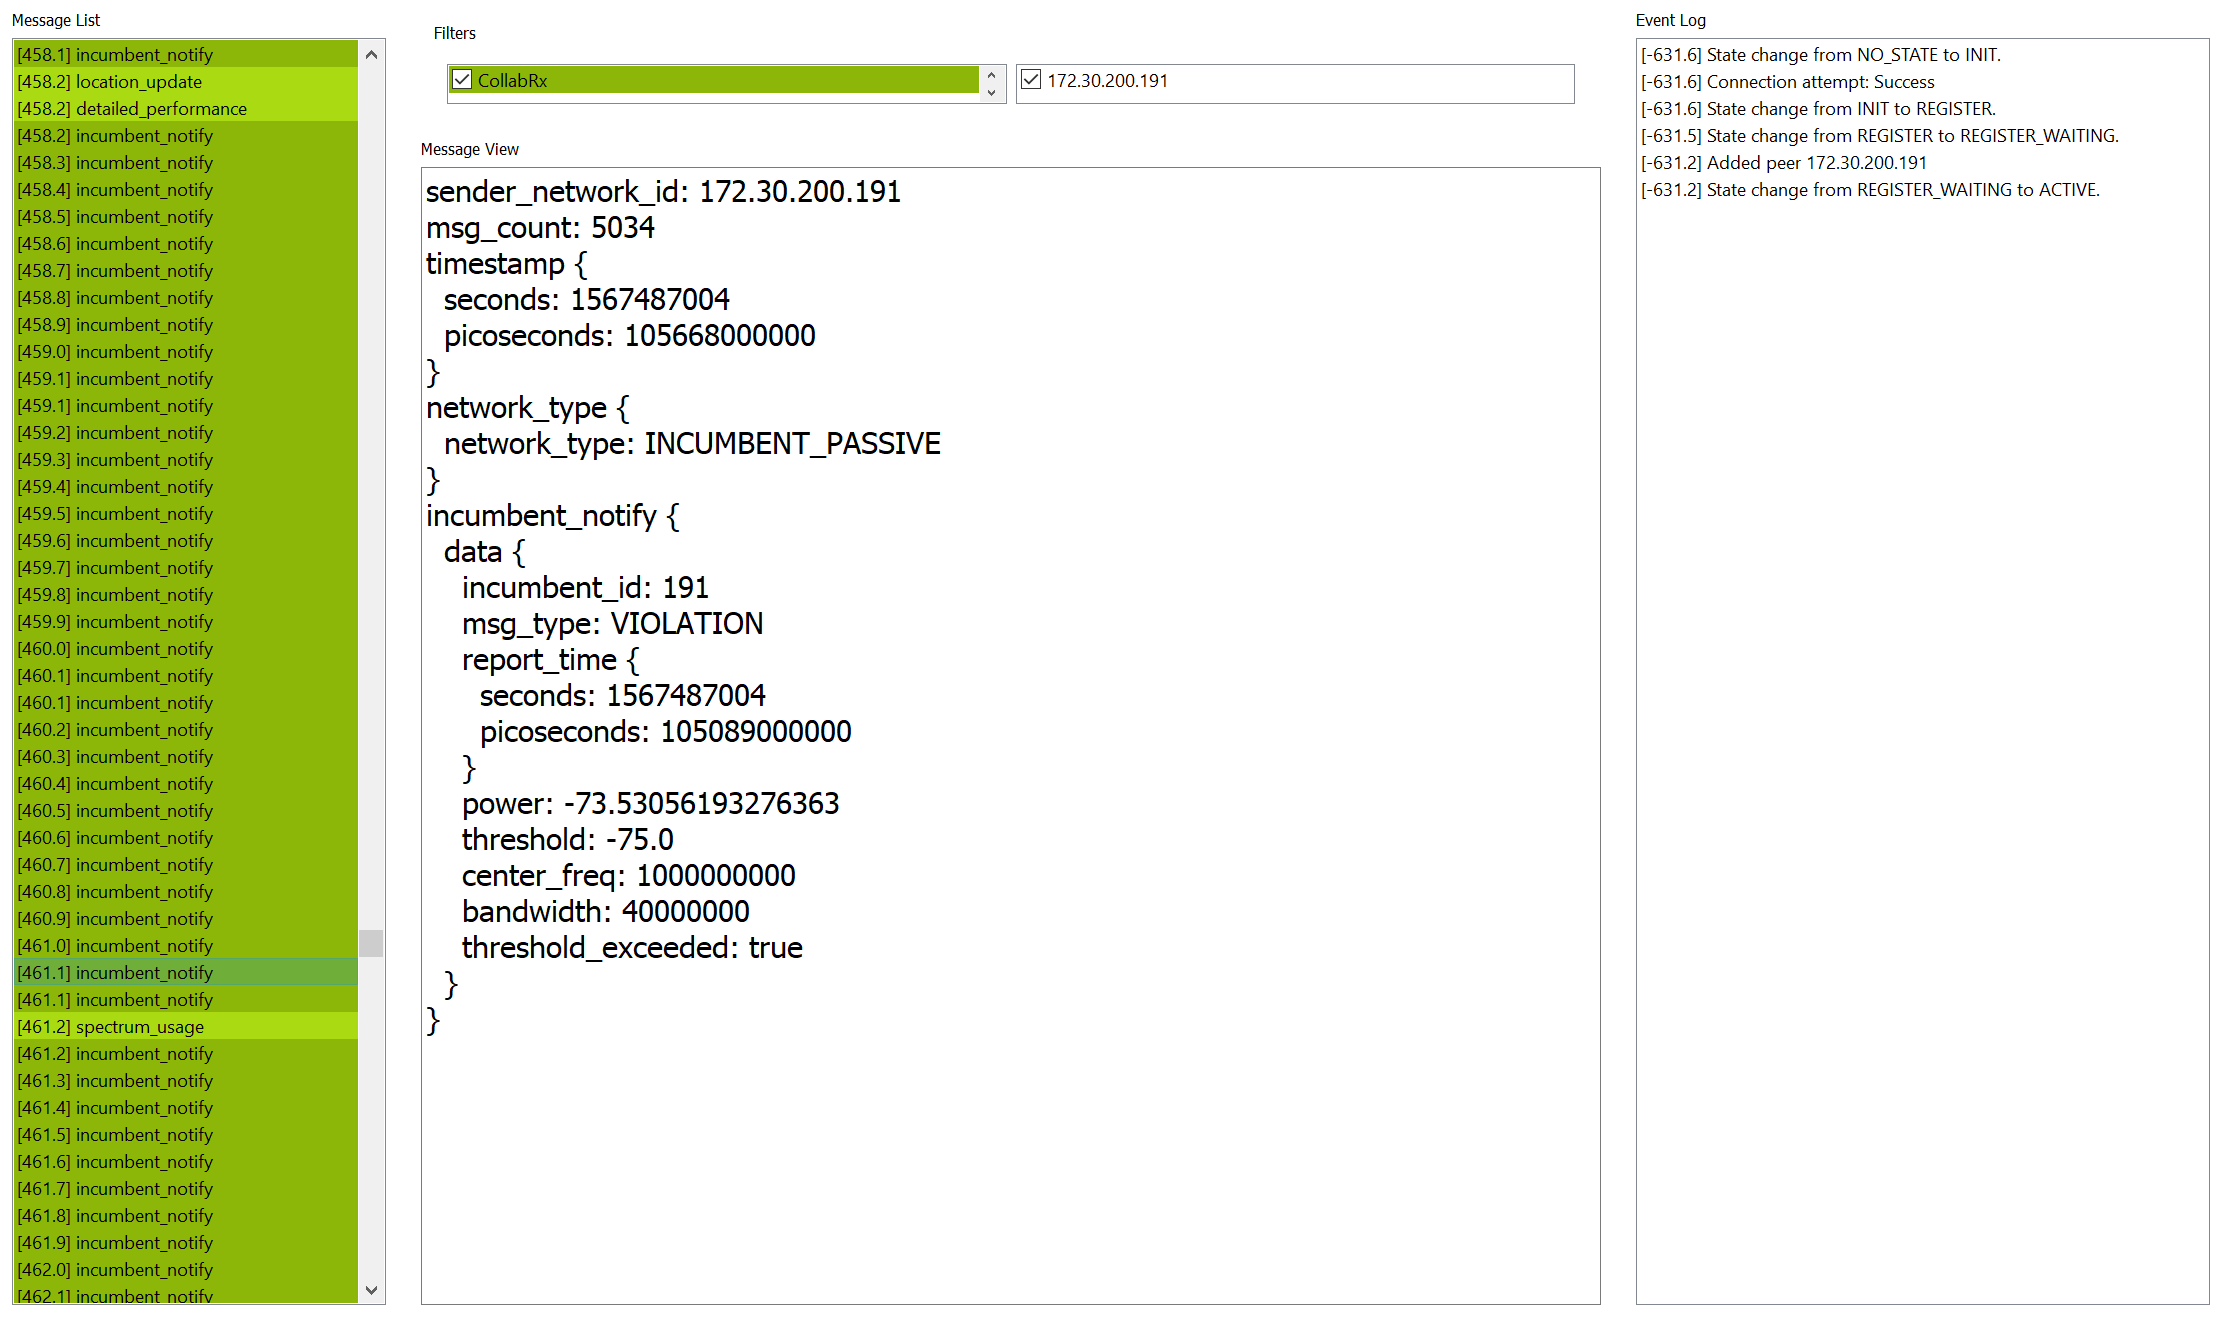
\includegraphics[width = 0.95\textwidth]{Passive_Incumbent_1.jpg}
    \caption{A Violation collaboration message from the Passive Incumbent}
    \label{fig:3}
\end{figure}
\end{frame}
\begin{frame}{PHY: Transmission Power Control (4/4)}
\begin{figure}
    \centering
    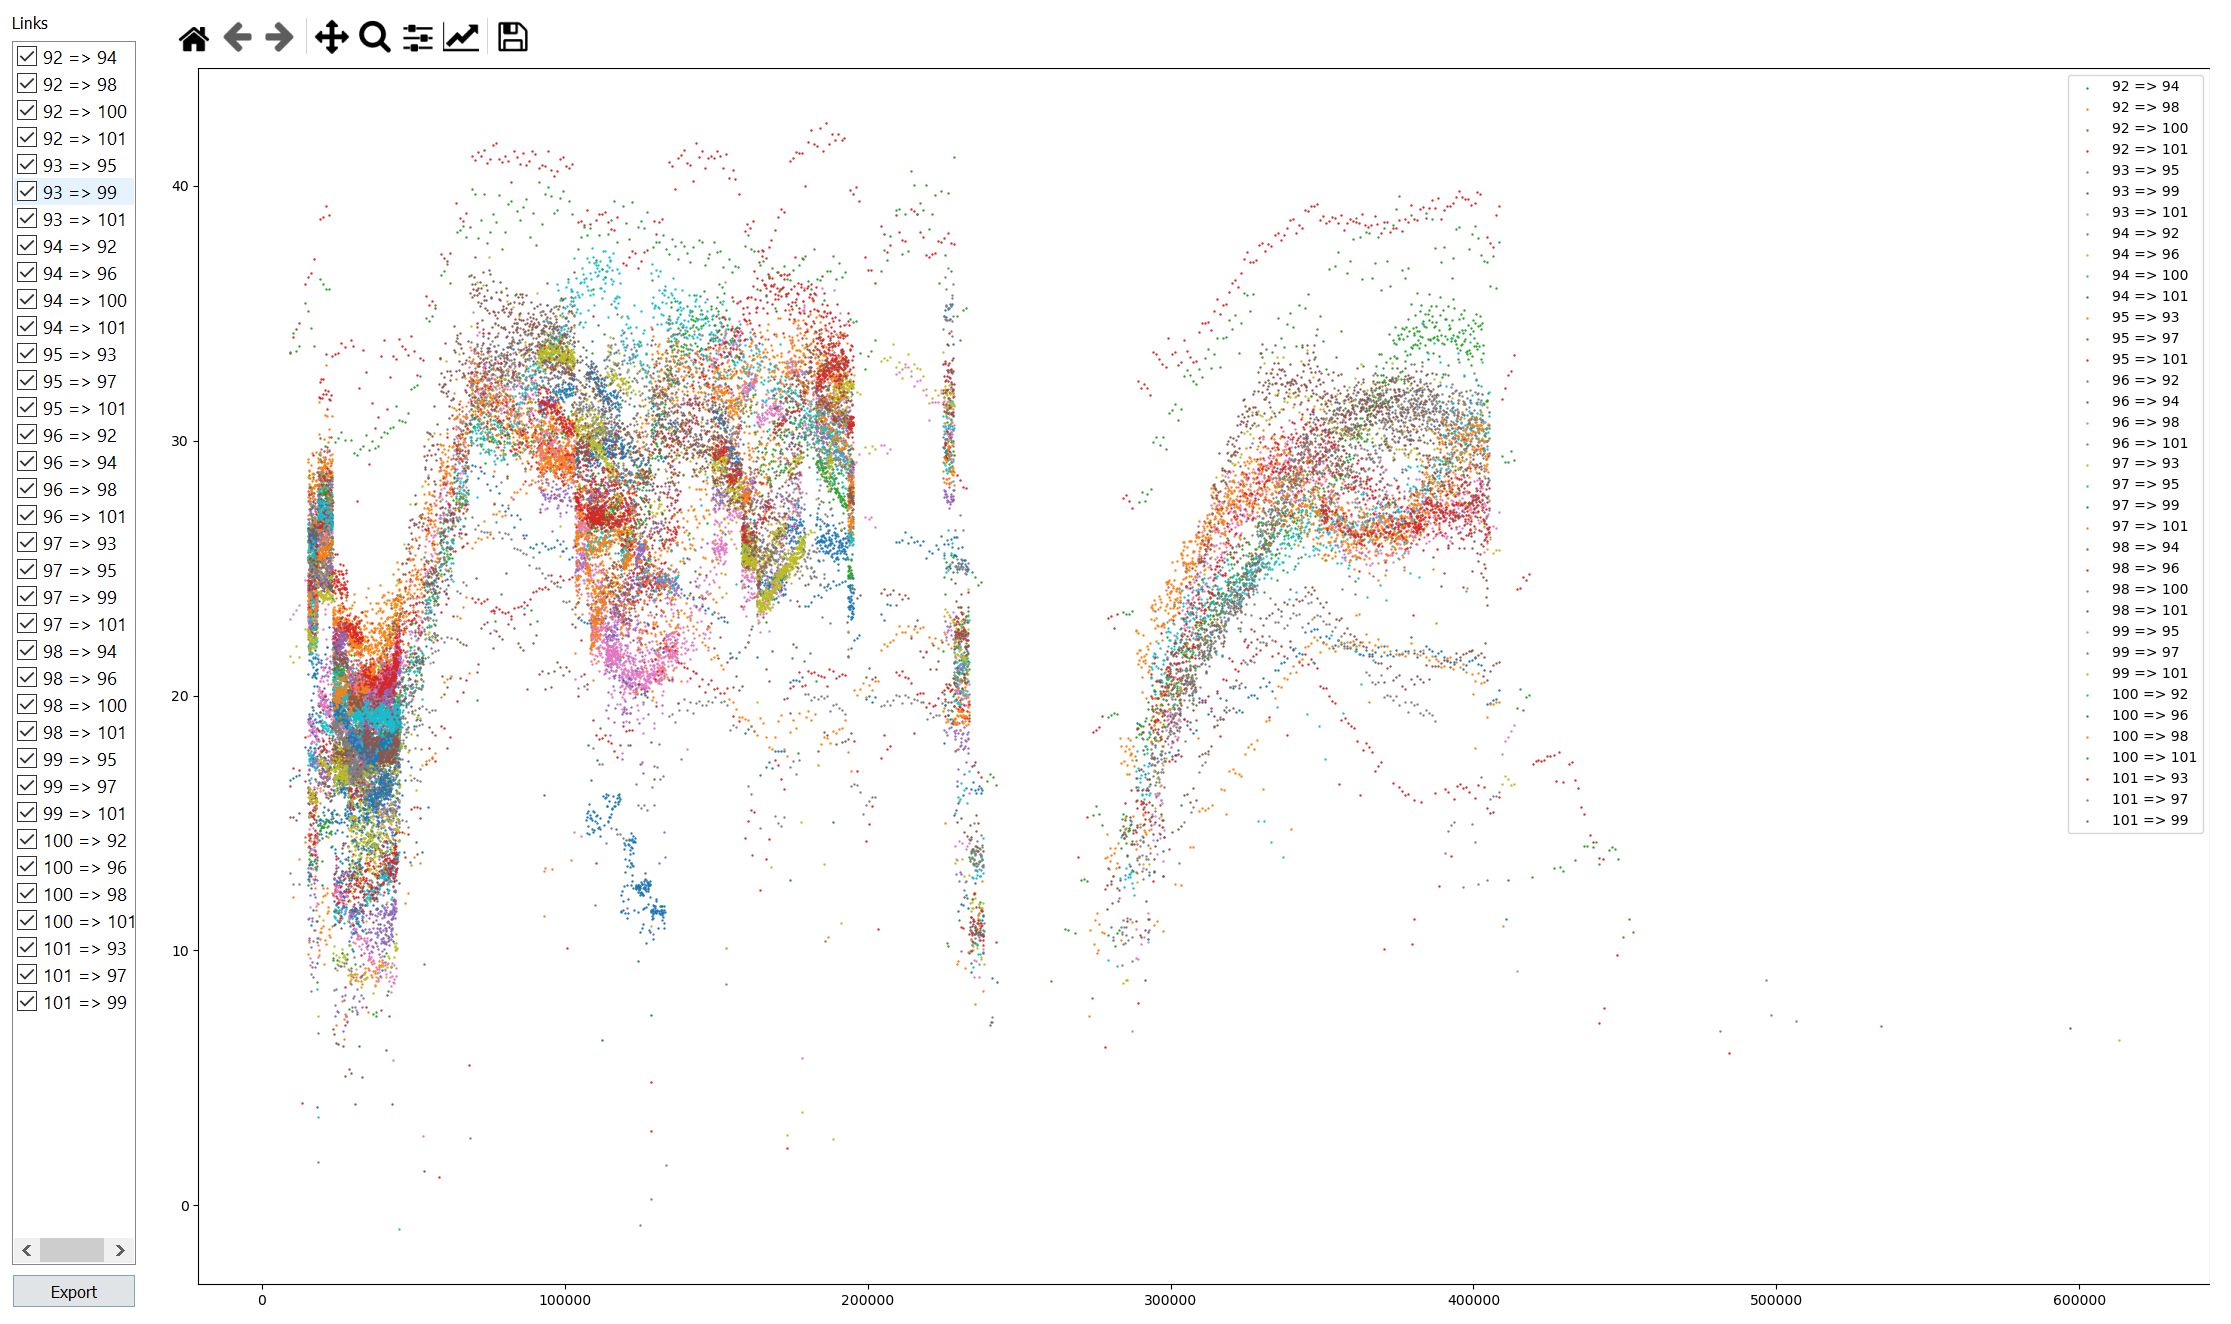
\includegraphics[width = 0.95\textwidth]{Passive_Incumbent_2.jpg}
    \caption{A significant drop in SNR due to Tx power attenuation across the BAM! Wireless Network}
    \label{fig:4}
\end{figure}
\end{frame}
\begin{frame}{PHY: The FSK Control Channel (1/2)}
    \begin{itemize}
        \item Short control message: number of SRNs, channel allocation, timestamp
        \item Network bootstrapping, Initial node discovery, Backup control link for all control messages (short + long) in high interference environments
        \item Non-coherent $8$-FSK link with $480$kHz of bandwidth
        \item Slotted ALOHA (without CD and backoff): at the slot boundary, each SRN transmits a short control message with a probability of $\frac{1}{\tilde{\Lambda}}$\texttt{-{}-}with these packets dropped at the receiver if there are decoding errors from collisions
        \item Time-slot period${=}60$ms
        \item Center frequency switches between the upper and lower spectral band-edges every second
    \end{itemize}
\end{frame}
\begin{frame}{PHY: The FSK Control Channel (2/2)}
\begin{figure}
    \centering
    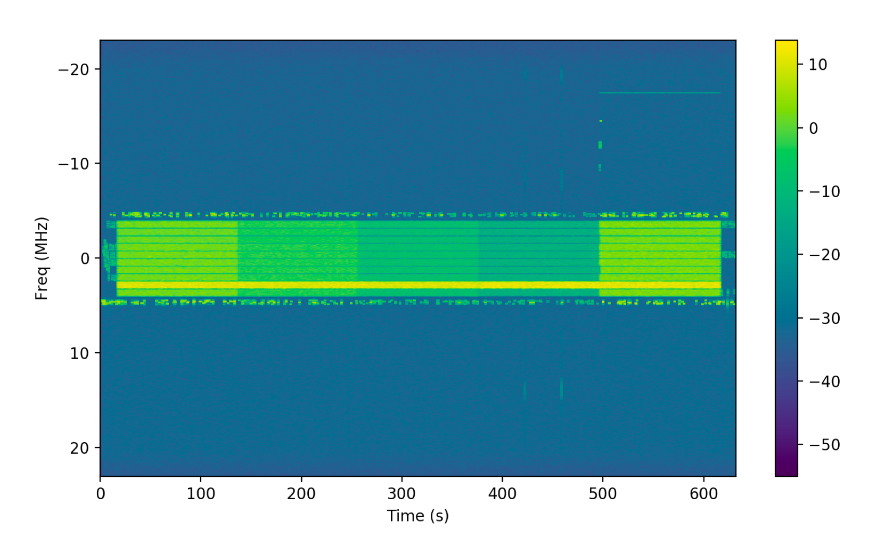
\includegraphics[width = 0.95\textwidth]{Control_Channels_At_Band_Edges.PNG}
    \caption{The FSK control channel at the upper and lower spectral band-edges during an SC$2$ Qualification scenario}
    \label{fig:5}
\end{figure}
\end{frame}
\begin{frame}{PHY: The DFT-s-OFDM Data Channel (1/2)}
    \footnotesize{\begin{itemize}
        \item Long control messages (traffic stats, perf. feedback) + traffic
        \item SRN: center-frequency assignment (GW channel allocation)
        \item SRN: channel BW determination (GW BW allocation)
        \item Each SRN tunes its $\tilde{\Lambda}{-}1$ receive chains to the Tx center frequency and BW of the other $\tilde{\Lambda}{-}1$ SRNs in the network
        \item $128$ sub-carriers: $108$ for data symbols, $12$ for pilot symbols, and $8$ for null transmissions (for noise variance estimation)
        \item Schmidl \& Cox time sync and freq. offset compensation
        \item Allowed modulation: QPSK, QAM$16$, QAM$32$, and QAM$64$
        \item Allowed code rates: $\frac{1}{2}$, $\frac{2}{3}$, $\frac{3}{4}$, and $\frac{5}{6}$ (IEEE 802.11 QC-LDPC)
        \item Frame Headers: rate $\frac{1}{2}$ LDPC with QPSK; source SRN ID, dest. SRN ID, MCS index, and number of blocks in the payload; $32$-bit CRC; Frame-ID for logging
        \item A sequence of DLL segments$\longrightarrow$a sequence of payload blocks (code-words)$\longrightarrow$modulated and mapped to a sequence of OFDM symbols on the sub-carriers
    \end{itemize}}
\end{frame}
\begin{frame}{PHY: The DFT-s-OFDM Data Channel (2/2)}
\begin{figure}
    \centering
    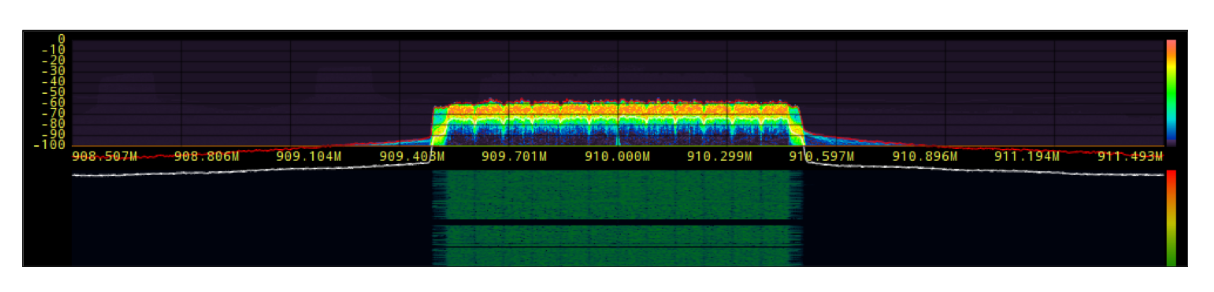
\includegraphics[width = 1.0\textwidth]{Data_Channel_DFT-spread-OFDM_Power_Spectrum.PNG}
    \caption{The FSK control channel at the upper and lower spectral band-edges during an SC$2$ Qualification scenario}
    \label{fig:6}
\end{figure}
\end{frame}
\begin{frame}{PHY: MCS Adaptation (1/5)}
    \footnotesize{\begin{itemize}
        \item Joint selection of modulation order $\mathcal{M}$ and code-rate $\mathcal{R}$ to maximize the raw throughput of a link
        \item Find the $(\mathcal{M},\mathcal{R})$ pair that has the smallest Euclidean distance between two circles centered about consecutive constellation symbols
        \item Radius of each of these circles proportional to the ratio of estimated noise (+interference) standard deviation to the asymptotic code gain
        \item Sliding window median filter applied to the estimated noise variance samples to remove samples with low probability of occurrence
        \item Optimization problem constraints: $(\mathcal{M},\mathcal{R})$-throughput should be above a threshold (QoS), and $(\mathcal{M},\mathcal{R})$-BLER should be below a threshold (closed-form approx.)
        \item \[\min_{\mathcal{M},\mathcal{R}}\ d_{\text{min}}(\mathcal{M},\mathcal{R},\hat{\sigma}) \text{ subject to}\ \rho_{l} \geq \rho_{l,\text{min}},\text{ and}\ \mathbb{P}_{b}^{(l)} \leq \mathbb{P}_{b}^{(l,\text{max})}\]
        \item \[\mathbb{P}_{b}^{(l)}=Q\left(\frac{d_{\text{min}}}{\sqrt{2\hat{\sigma}^{2}}}\right),\text{ if $\mathcal{M}=4$};\ \mathbb{P}_{b}^{(l)}=\frac{4}{\log_{2}(\mathcal{M})}Q\left(\frac{d_{\text{min}}}{\sqrt{2\hat{\sigma}^{2}}}\right),\text{ if $\mathcal{M}>4$}\]
        \item \[\rho_{l}=\mathcal{R} \cdot BW_{l} \cdot \log_{2}(\mathcal{M})\]
    \end{itemize}}
\end{frame}
\begin{frame}{PHY: MCS Adaptation (2/5)}
\begin{figure}
    \centering
    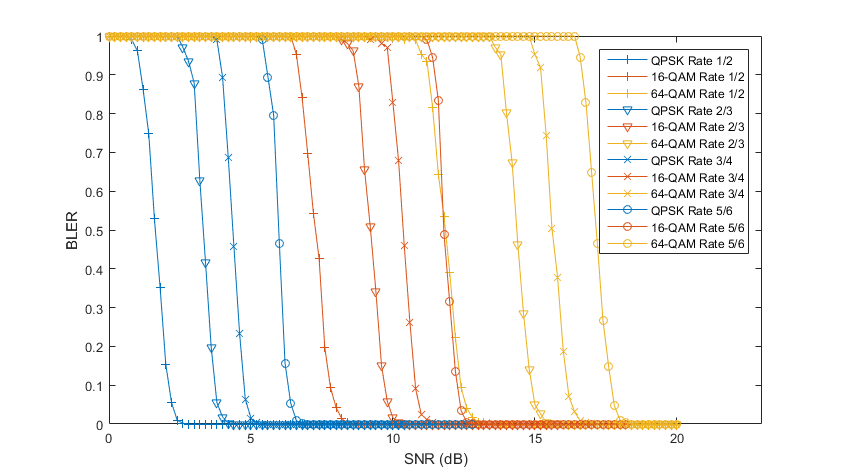
\includegraphics[width = 0.95\textwidth]{BLER.png}
    \caption{Simulated BLER curves for different combinations of modulation order and code rate}
    \label{fig:7}
\end{figure}
\end{frame}
\begin{frame}{PHY: MCS Adaptation (3/5)}
\begin{figure}
    \centering
    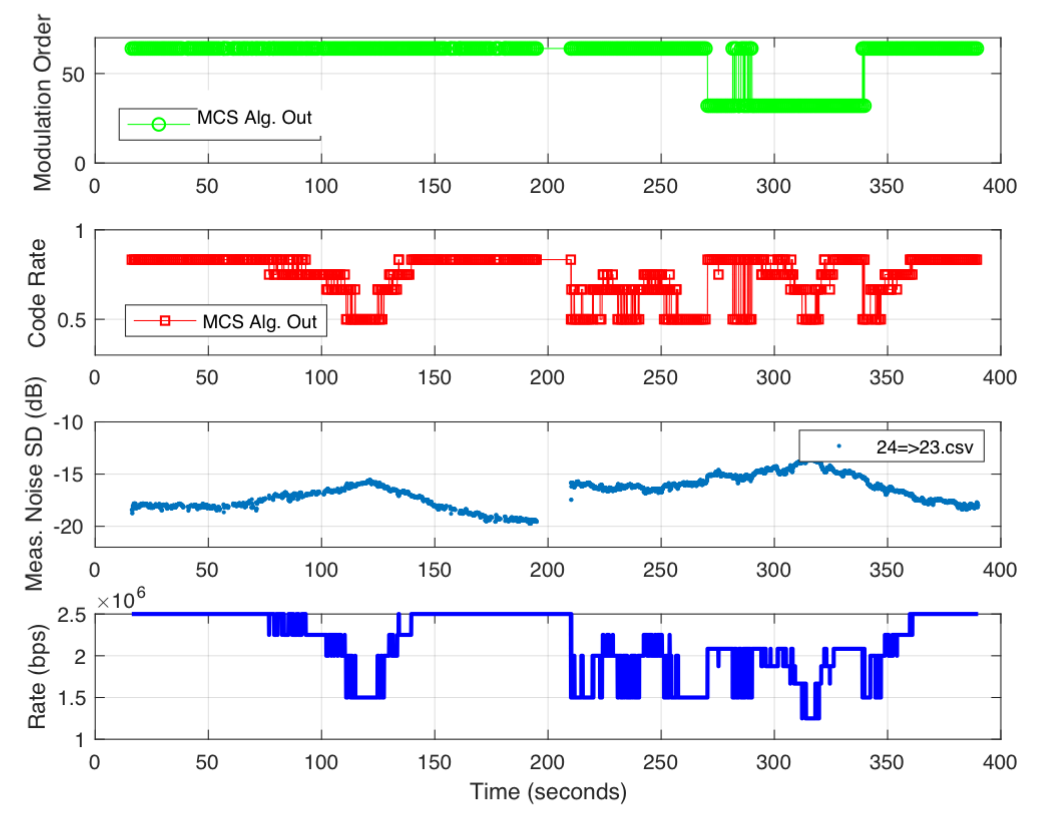
\includegraphics[width = 0.75\textwidth]{Payline_MCS_Adaptation.PNG}
    \caption{MCS adaptation to changes in noise variance during an SC$2$ Payline scenario}
    \label{fig:8}
\end{figure}
\end{frame}
\begin{frame}{PHY: MCS Adaptation (4/5)}
\begin{figure}
    \centering
    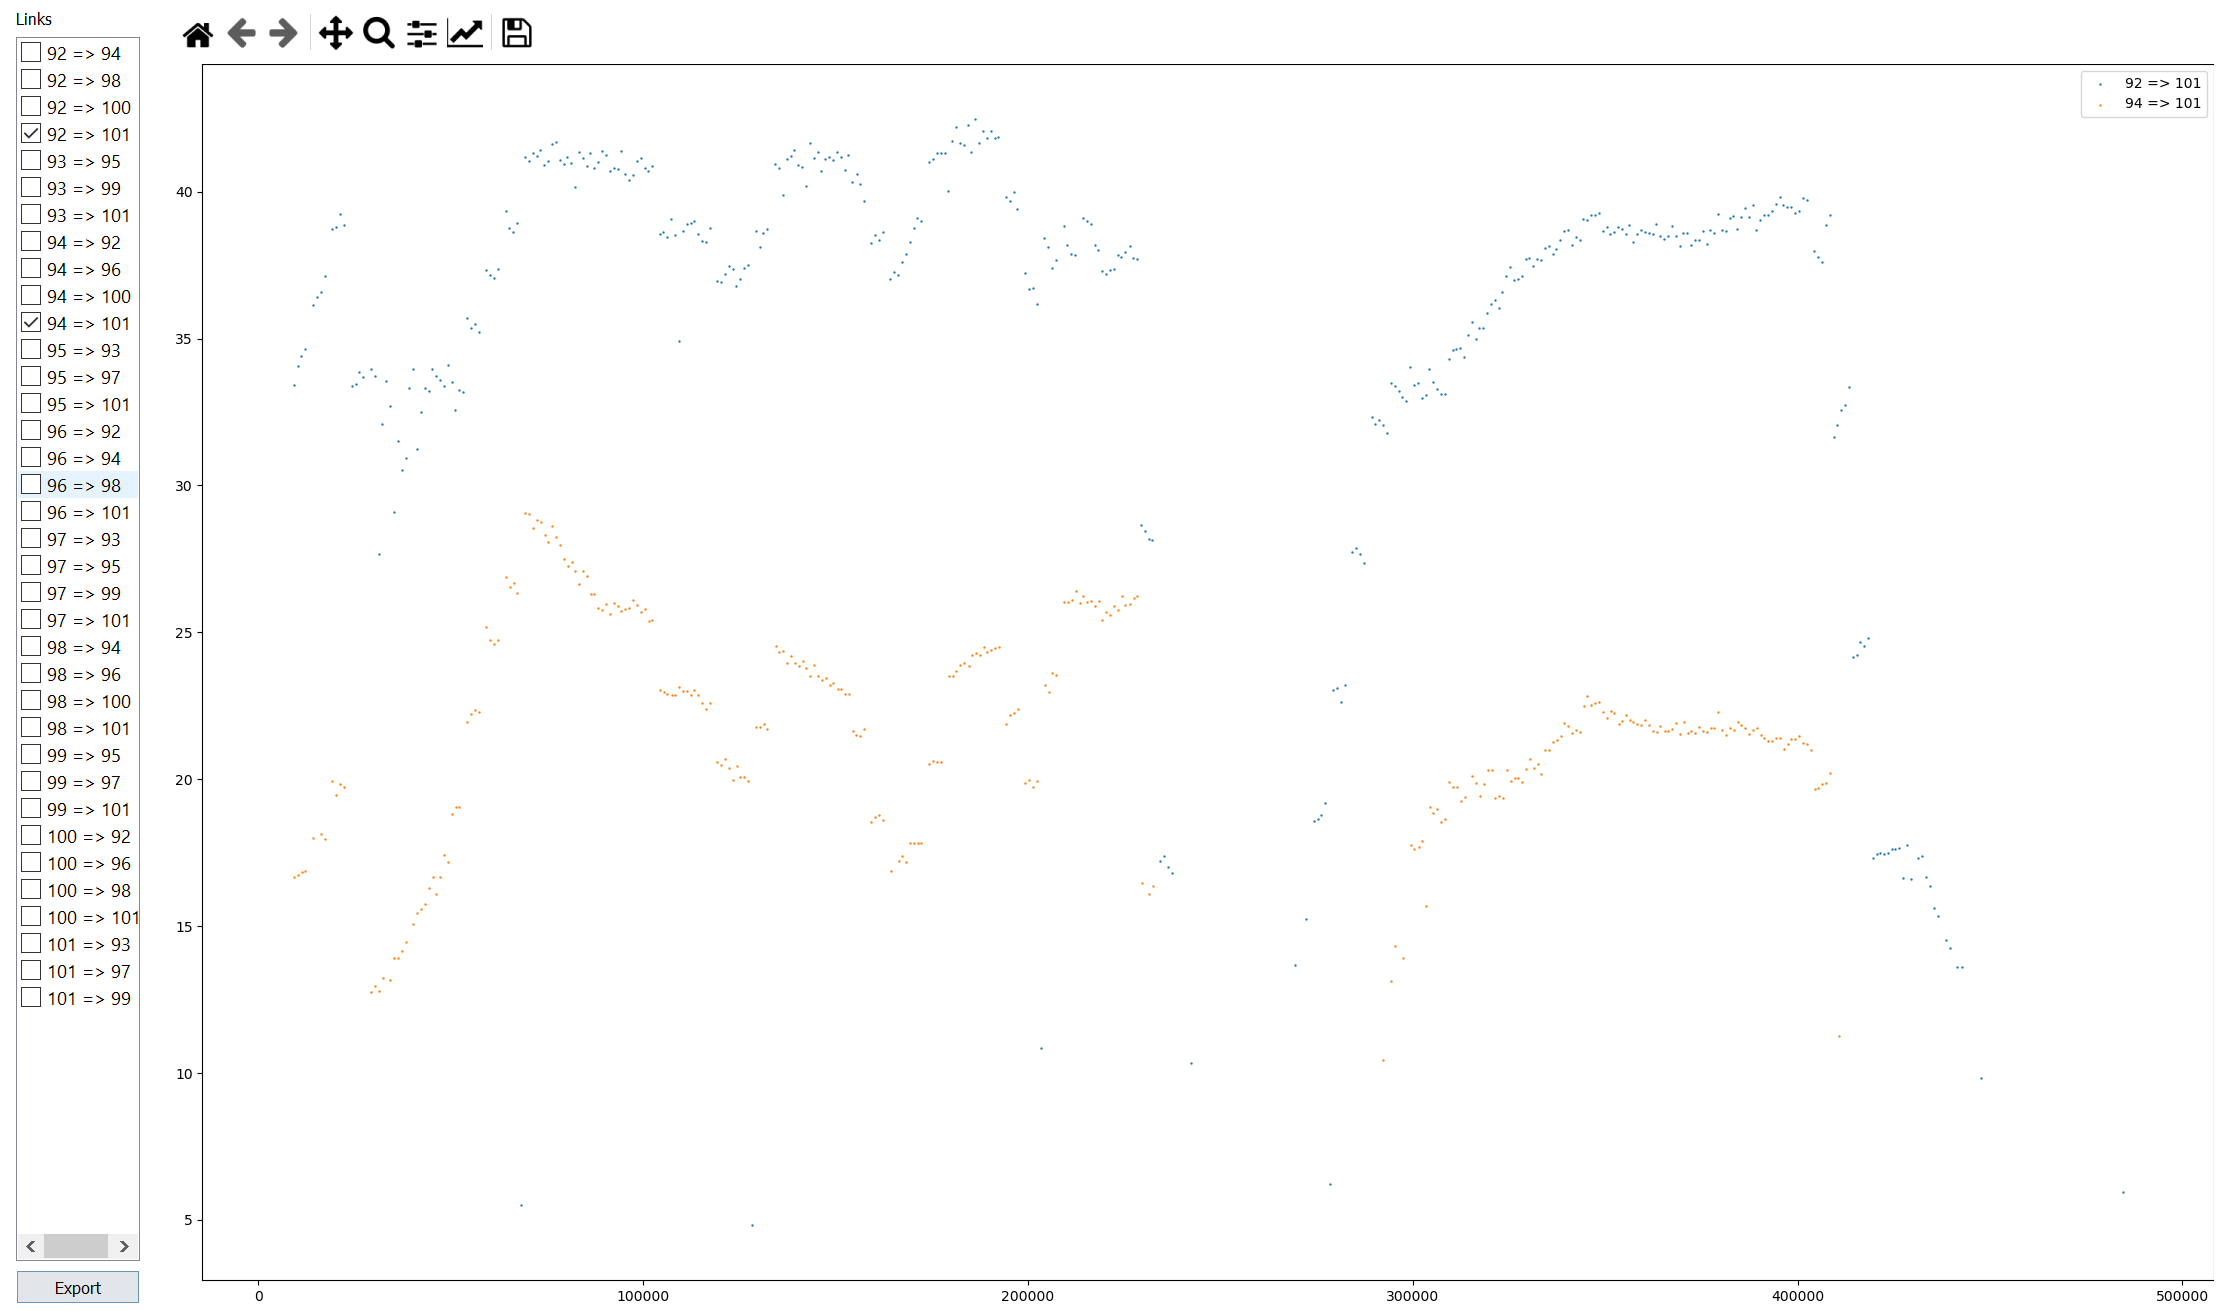
\includegraphics[width = 0.95\textwidth]{Alleys_MCS_2.PNG}
    \caption{The SNR variations for two specific links during an SC$2$ Alleys of Austin scenario}
    \label{fig:9}
\end{figure}
\end{frame}
\begin{frame}{PHY: MCS Adaptation (5/5)}
\begin{figure}
    \centering
    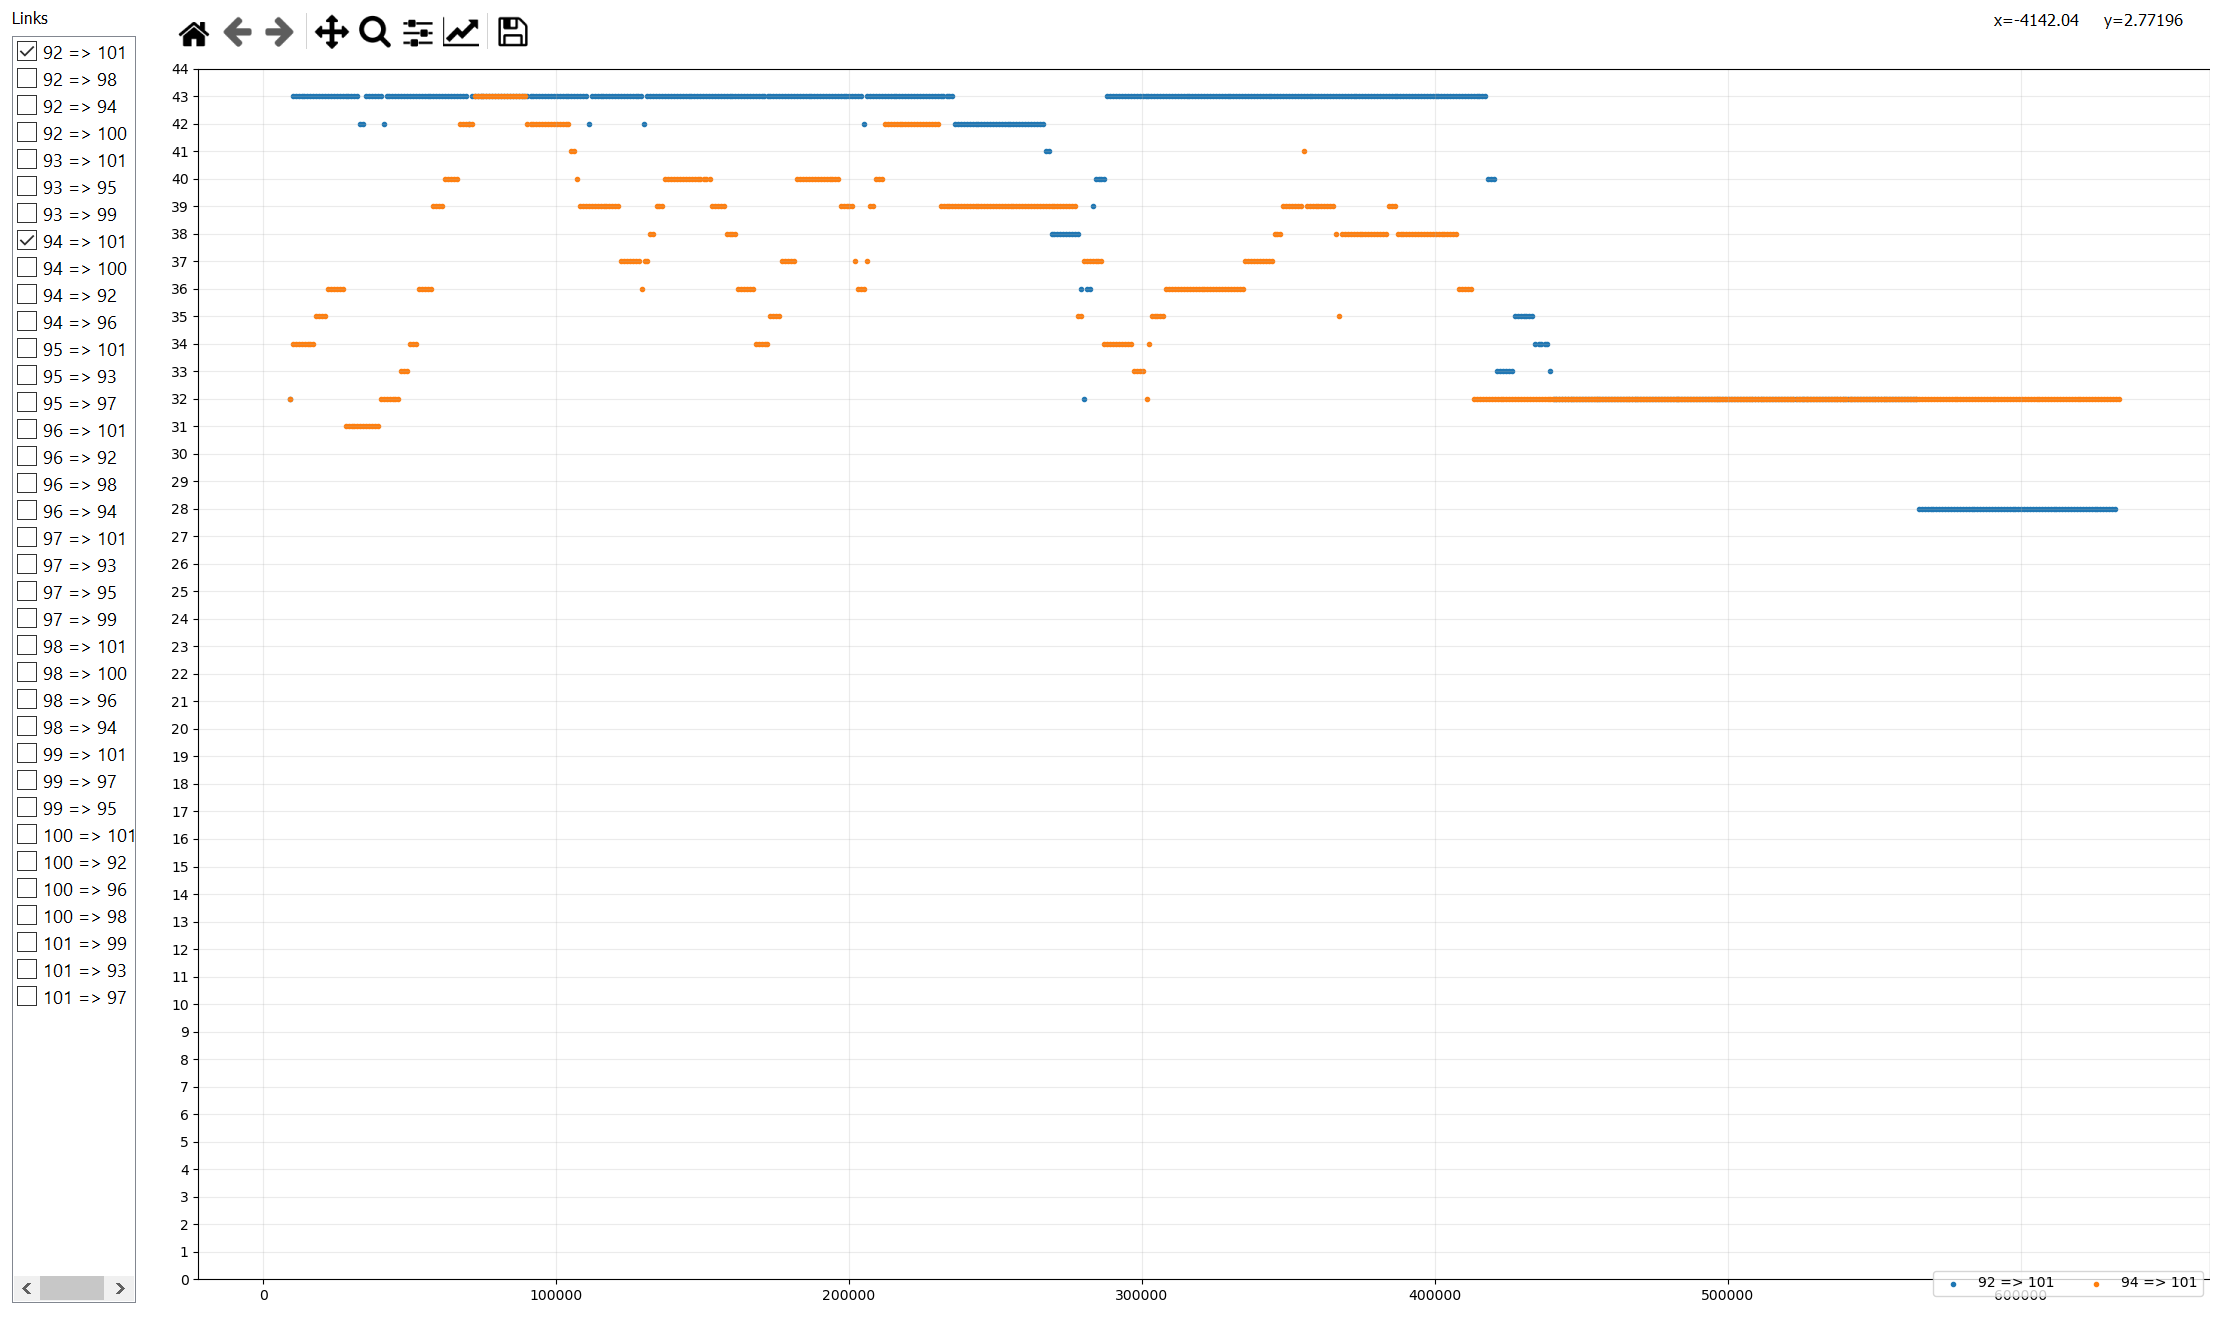
\includegraphics[width = 0.90\textwidth]{Alleys_MCS_1.PNG}
    \caption{MCS adaptation w.r.t the two specific corresponding to changes in their estimated SNRs during an SC$2$ Alleys of Austin scenario: Highest MCS index $43{-}(\mathcal{M}{=}\text{QAM}64,\mathcal{R}{=}\frac{5}{6})$ and Lowest MCS index $28{-}(\mathcal{M}{=}\text{QPSK},\mathcal{R}{=}\frac{1}{2})$}
    \label{fig:10}
\end{figure}
\end{frame}
\begin{frame}{DLL: Prioritized Flow Scheduling with ARQ (1/4)}
    \footnotesize{\begin{itemize}
        \item VOIP${=}4$, UAV CCTV stream${=}9$, Video bombing run${=}15$ 
        \item Time-quanta based resource block termed a ``Quantum-Schedule" (QS)
        \item Deficit round-robin queueing using ``credits"
        \item ARQ only for file transfers: Detect bursty UDP flows$\longrightarrow$sequence the packets$\longrightarrow$the receiver ACKs for every sequence$\longrightarrow$unacknowledged packets are dynamically re-enqueued into a special ARQ queue for re-transmission by the scheduler
        \item New flows are enqueued in their own queues at the DLL of an SRN
        \item Schedule Update: Determine the upper and lower bounds of a QS using flow information and link quality
        \[t_{\text{min}}^{(f)}=\frac{f_{\text{ov}}+f_{\text{nseg}}(f_{\text{seg-ov}}+f_{\text{seg-bits}})}{\rho_{l_{f}}};\ \text{lb}_{i}=\sum_{f \in \mathcal{F}_{i}}t_{\text{min}}^{(f)};\ \text{ub}_{i}=\min_{f \in \mathcal{F}_{i}}\delta_{\text{max}}^{(f)}\]
        \item Rank the flows at the DLL of this SRN in the decreasing order of their value-per-resource metric
        \[\psi_{f}=\frac{V_{f}f_{\text{nseg}}(f_{\text{seg-bits}}-f_{\text{seg-payload-ov}})}{t_{\text{min}}^{(f)}\rho_{l_{f}}}\]
        \item Fit these flows into the resource block in the ranked order\texttt{-{}-}with recursive revisitation triggered if there are un-scheduled flows and available resources in the QS
    \end{itemize}}
\end{frame}
\begin{frame}{DLL: Prioritized Flow Scheduling with ARQ (2/4)}
\begin{figure}
    \centering
    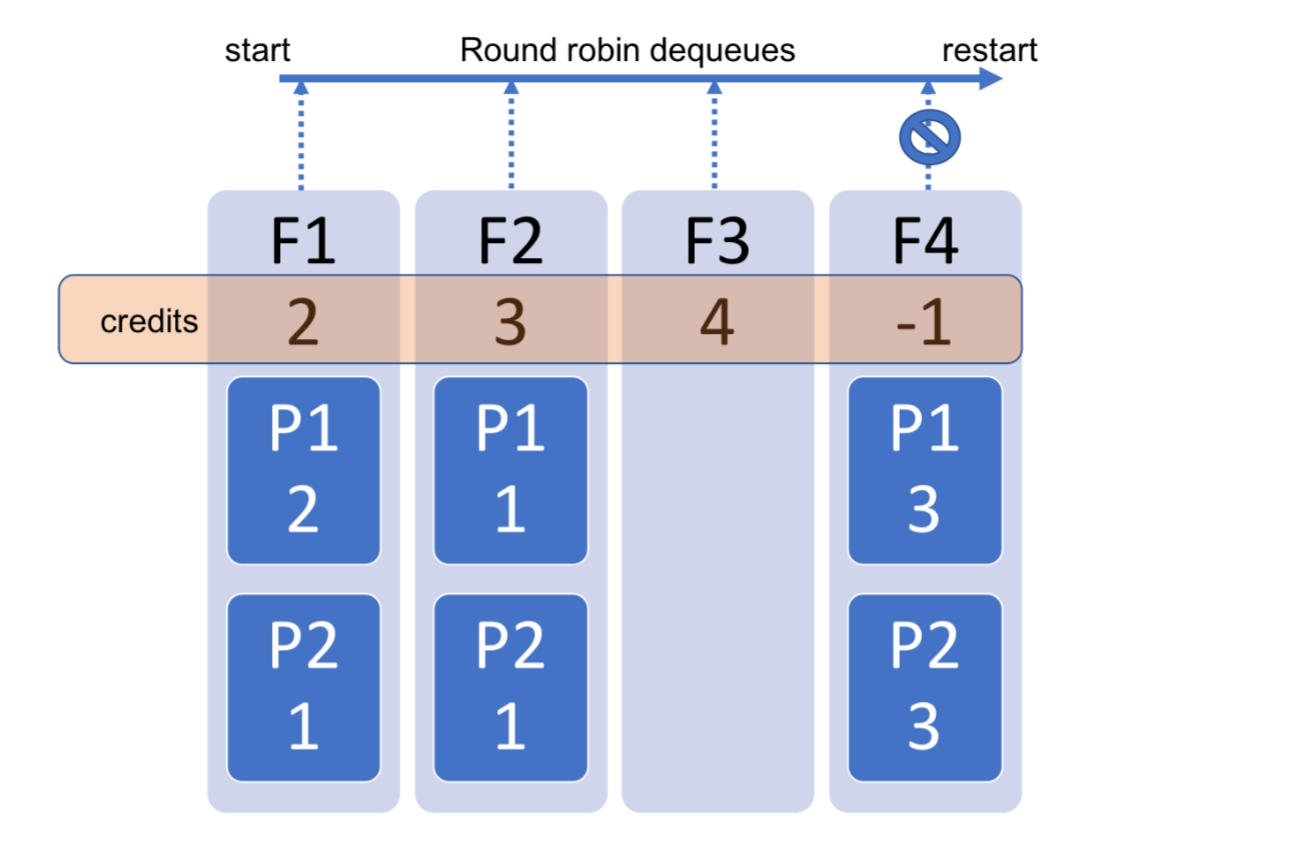
\includegraphics[width = 0.95\textwidth]{Deficit_Round_Robin_Scheduling.PNG}
    \caption{Deficit round-robin scheduling with a concept of ``credits"}
    \label{fig:11}
\end{figure}
\end{frame}
\begin{frame}{DLL: Prioritized Flow Scheduling with ARQ (3/4)}
\begin{figure}
    \centering
    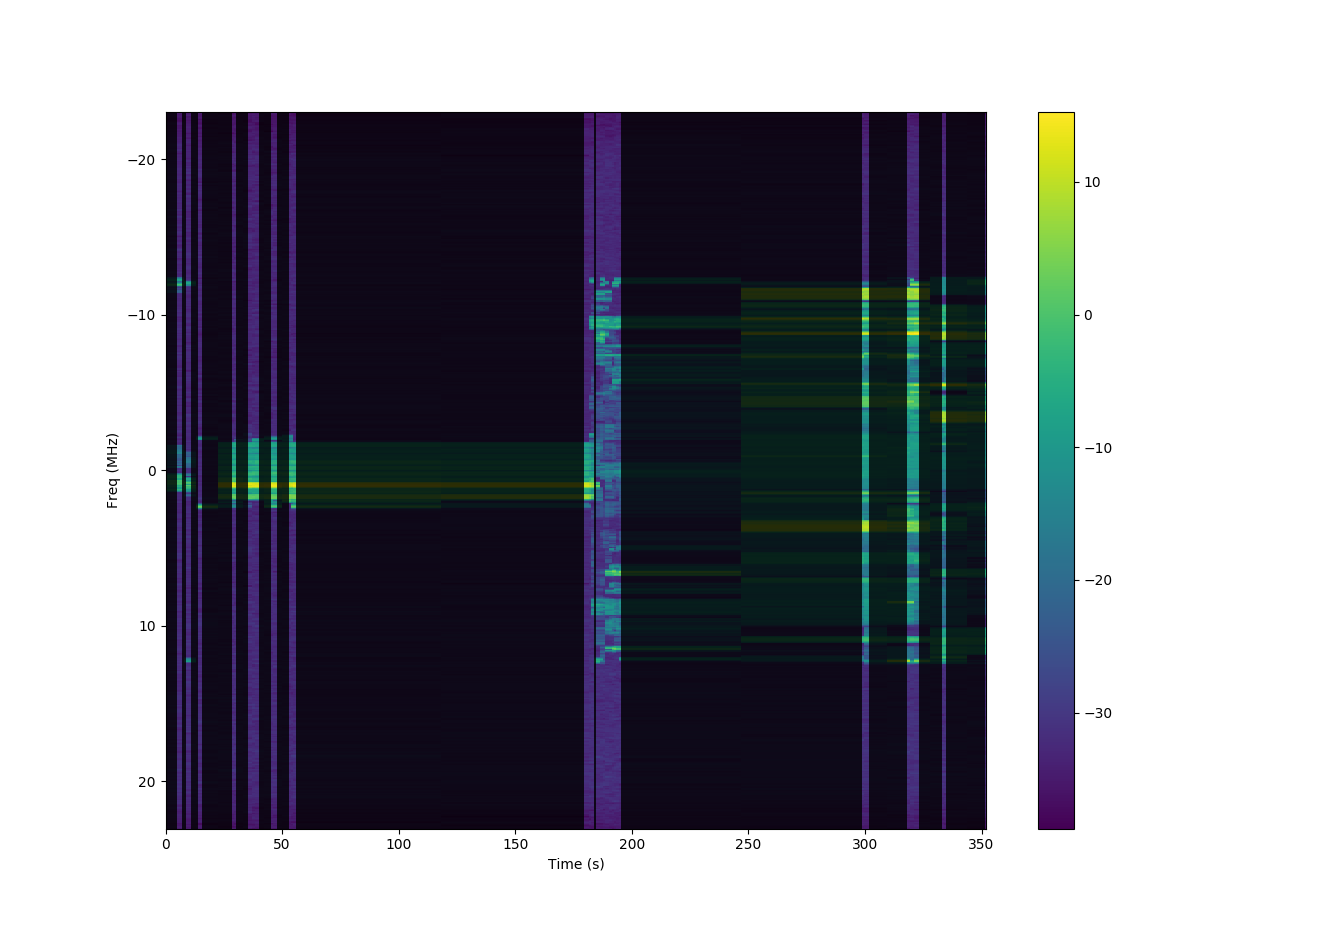
\includegraphics[width = 0.85\textwidth]{PSD_without_fix_payline.png}
    \caption{A situation in which PSD flows from an SRN (to the GW) are not prioritized over other flows during an SC$2$ Payline scenario}
    \label{fig:12}
\end{figure}
\end{frame}
\begin{frame}{DLL: Prioritized Flow Scheduling with ARQ (4/4)}
\begin{figure}
    \centering
    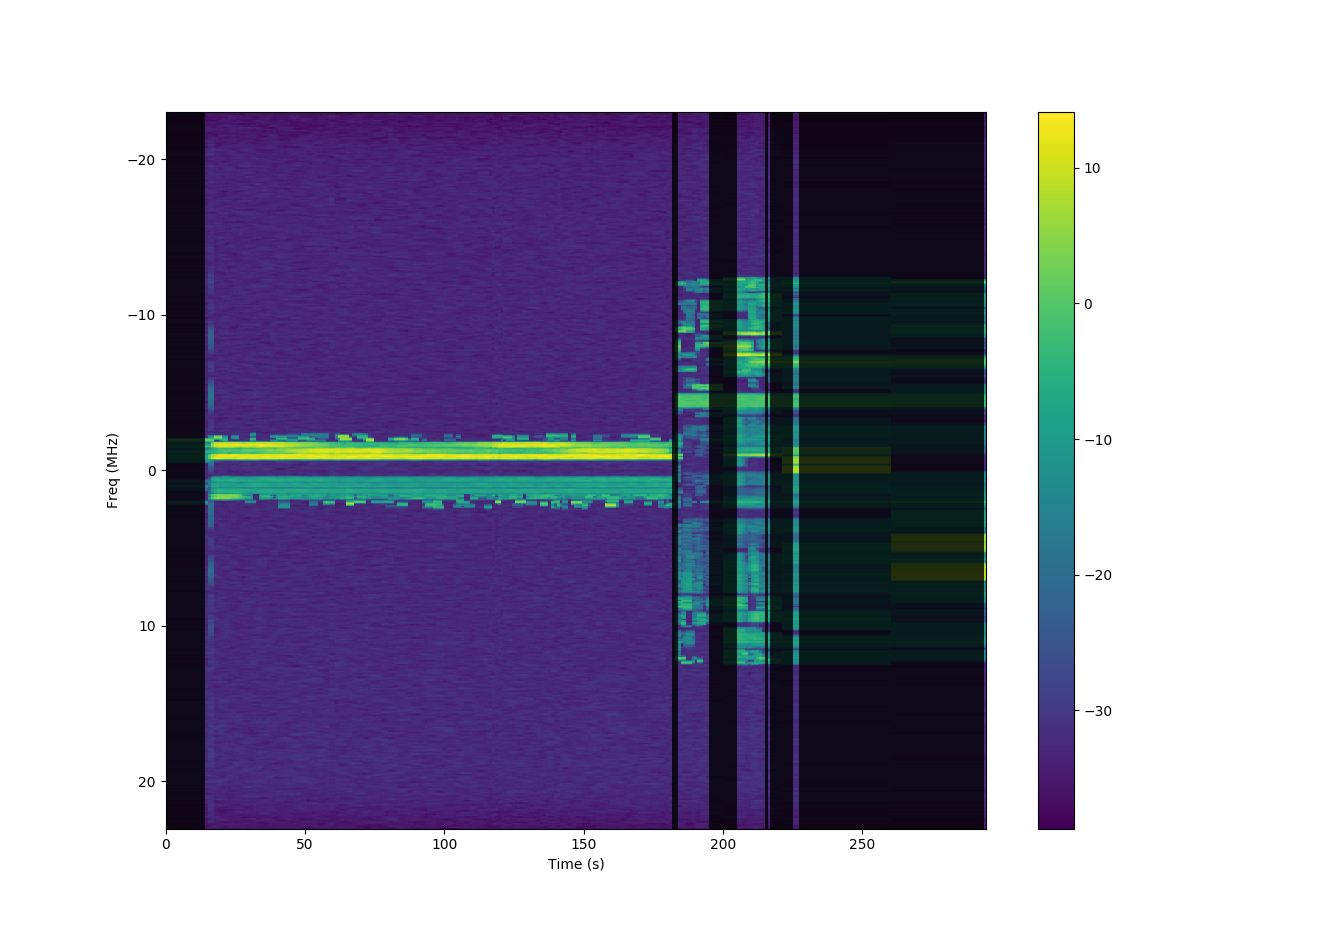
\includegraphics[width = 0.85\textwidth]{PSD_with_fix_payline.png}
    \caption{A situation in which PSD flows from an SRN (to the GW) are prioritized over most other flows during an SC$2$ Payline scenario: \textcolor{magenta}{leads to a drop in scores}}
    \label{fig:13}
\end{figure}
\end{frame}
\begin{frame}{MAC: BW and Channel Allocation (1/4)}
    \footnotesize{\begin{itemize}
        \item BW and channel allocation triggers: our scores and those of our competitors (sent over the collaboration network)\texttt{-{}-}in order to strike a balance between the ``self" and the ``team"; environment updates, and new flows/new mandates to existing flows
        \item BW allocation factors: amount of traffic at each link, QoS mandates for flows on this link, link quality, self and peer performance (from CIL messages)
        \item Channel allocation factors: PSD measurements, self and peer performance (from CIL messages), self and peer location information (from CIL messages), self and peer Tx power on the channels (from CIL messages)
        \item First, estimate the channel gain on each link based on their location and the path loss exponent
        \item Second, estimate the amount of interference caused to our transmissions on a channel based on the estimated channel gain, the location of interfering SRNs, and the Tx power of these interfering SRNs
        \item Finally, perform a heuristic search to determine the center frequencies that minimize this interference at our SRN receivers
    \end{itemize}}
\end{frame}
\begin{frame}{MAC: BW and Channel Allocation (2/4)}
\begin{figure}
    \centering
    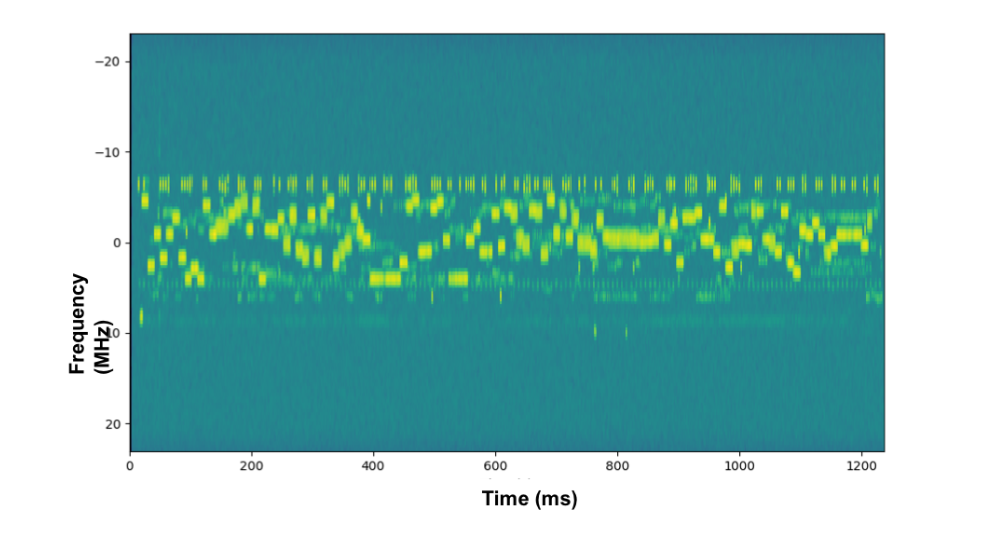
\includegraphics[width = 0.95\textwidth]{Alleys_of_Austin_Channel_Access.PNG}
    \caption{The spectrum occupied by our SRNs (time-frequency map) with re-allocations triggered by a combination of local PSD obs and CIL msgs, during an SC$2$ Alleys of Austin scenario}
    \label{fig:14}
\end{figure}
\end{frame}
\begin{frame}{MAC: BW and Channel Allocation (3/4)}
\begin{figure}
    \centering
    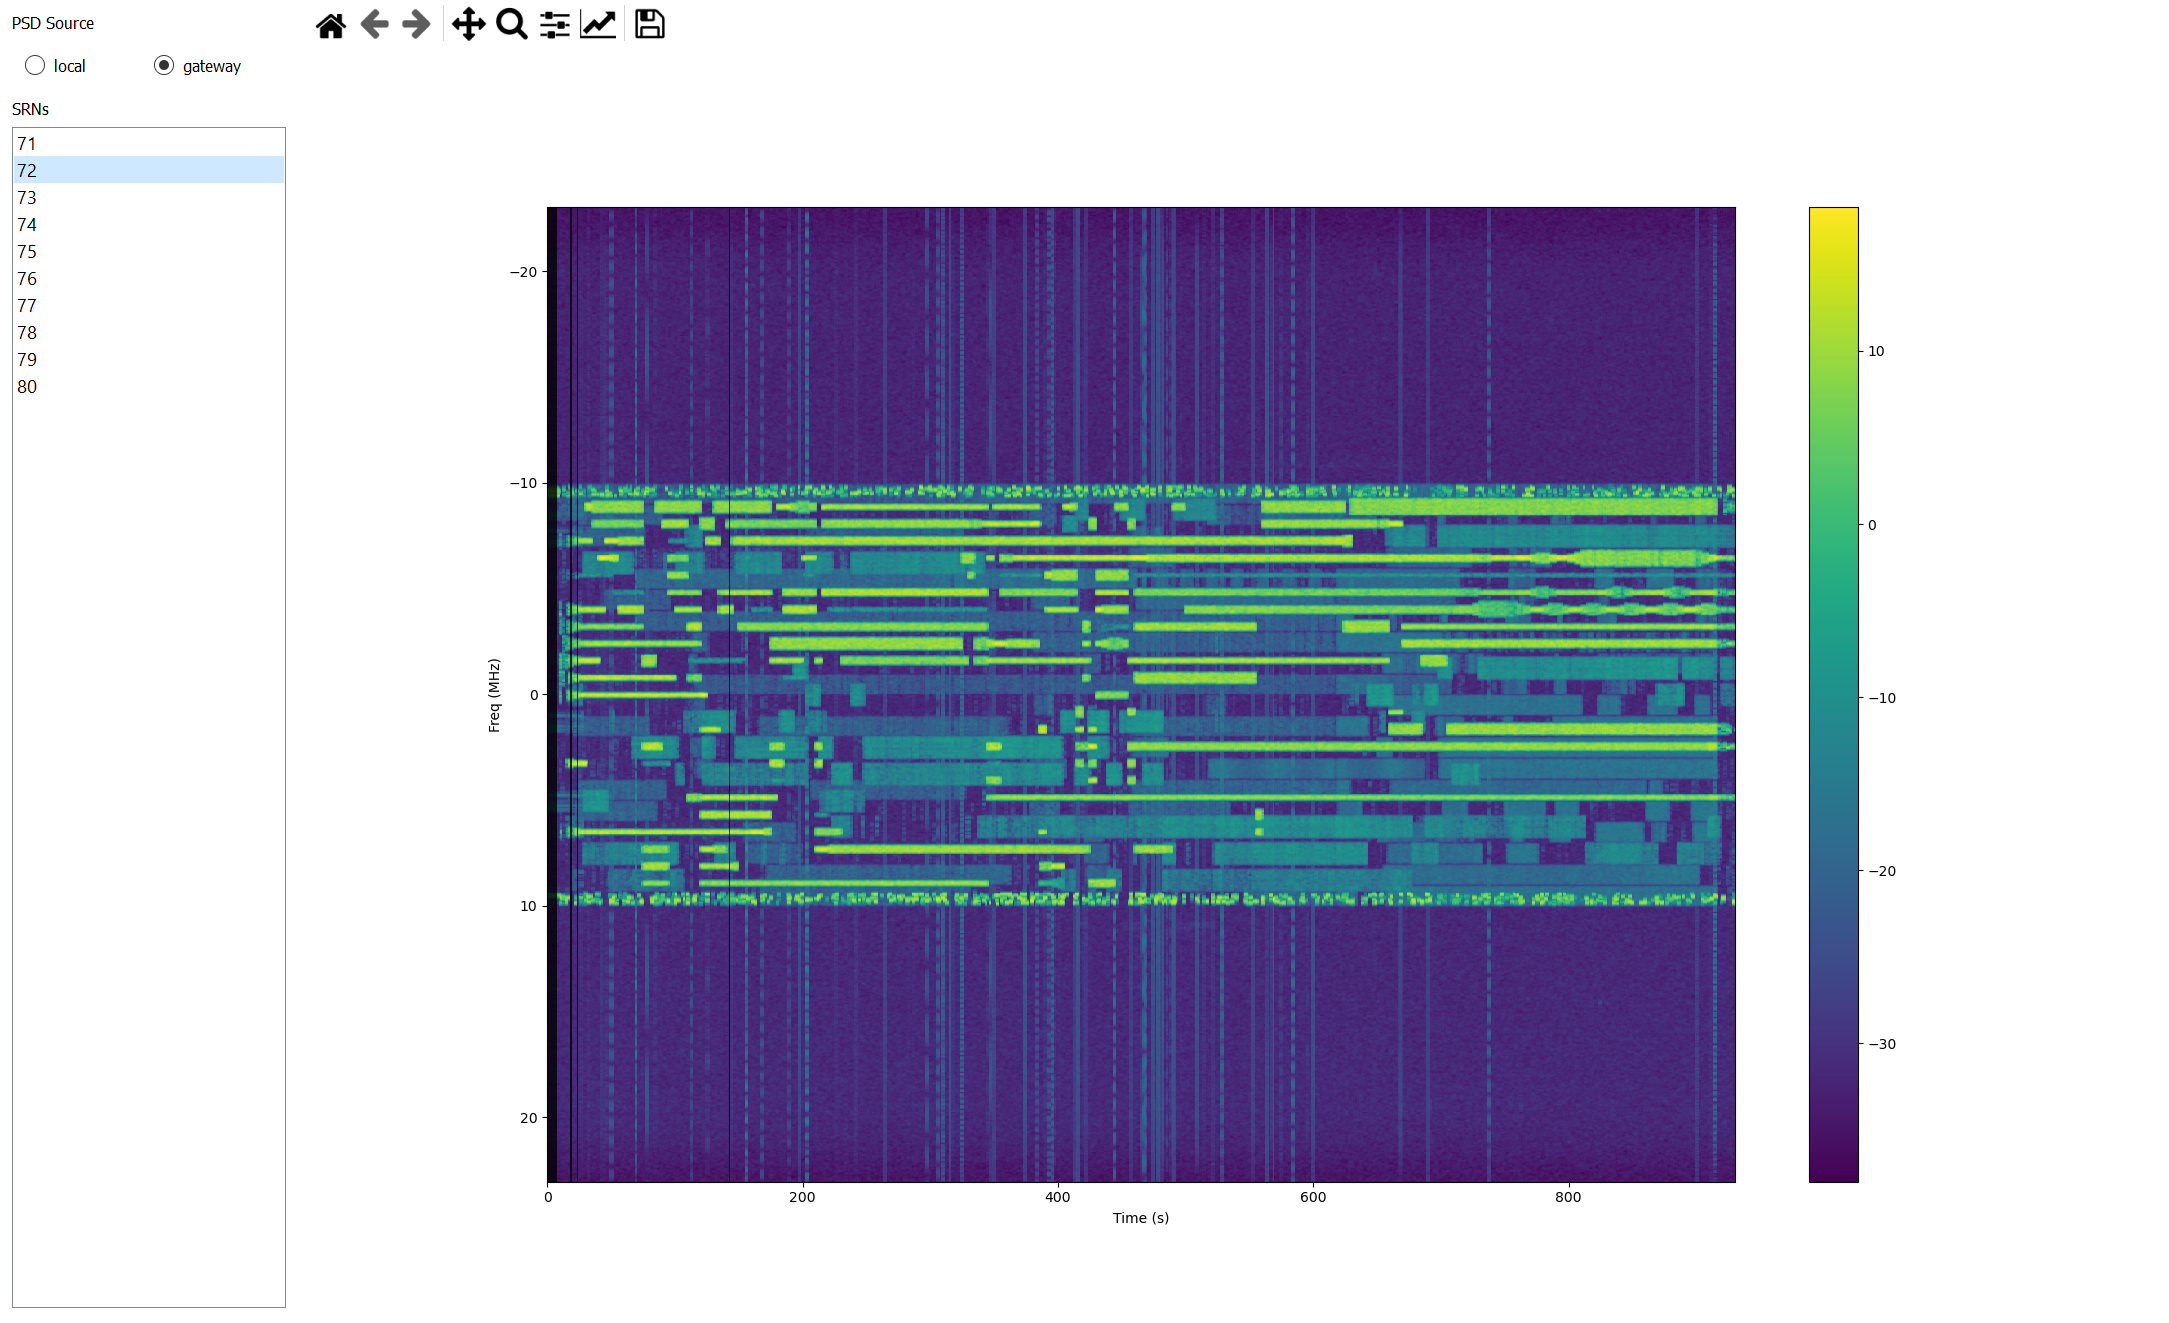
\includegraphics[width = 0.95\textwidth]{Alleys_PSD.PNG}
    \caption{The PSD observations from SRN $72$ to our GW during an SC$2$ Alleys of Austin scenario}
    \label{fig:15}
\end{figure}
\end{frame}
\begin{frame}{MAC: BW and Channel Allocation (4/4)}
\begin{figure}
    \centering
    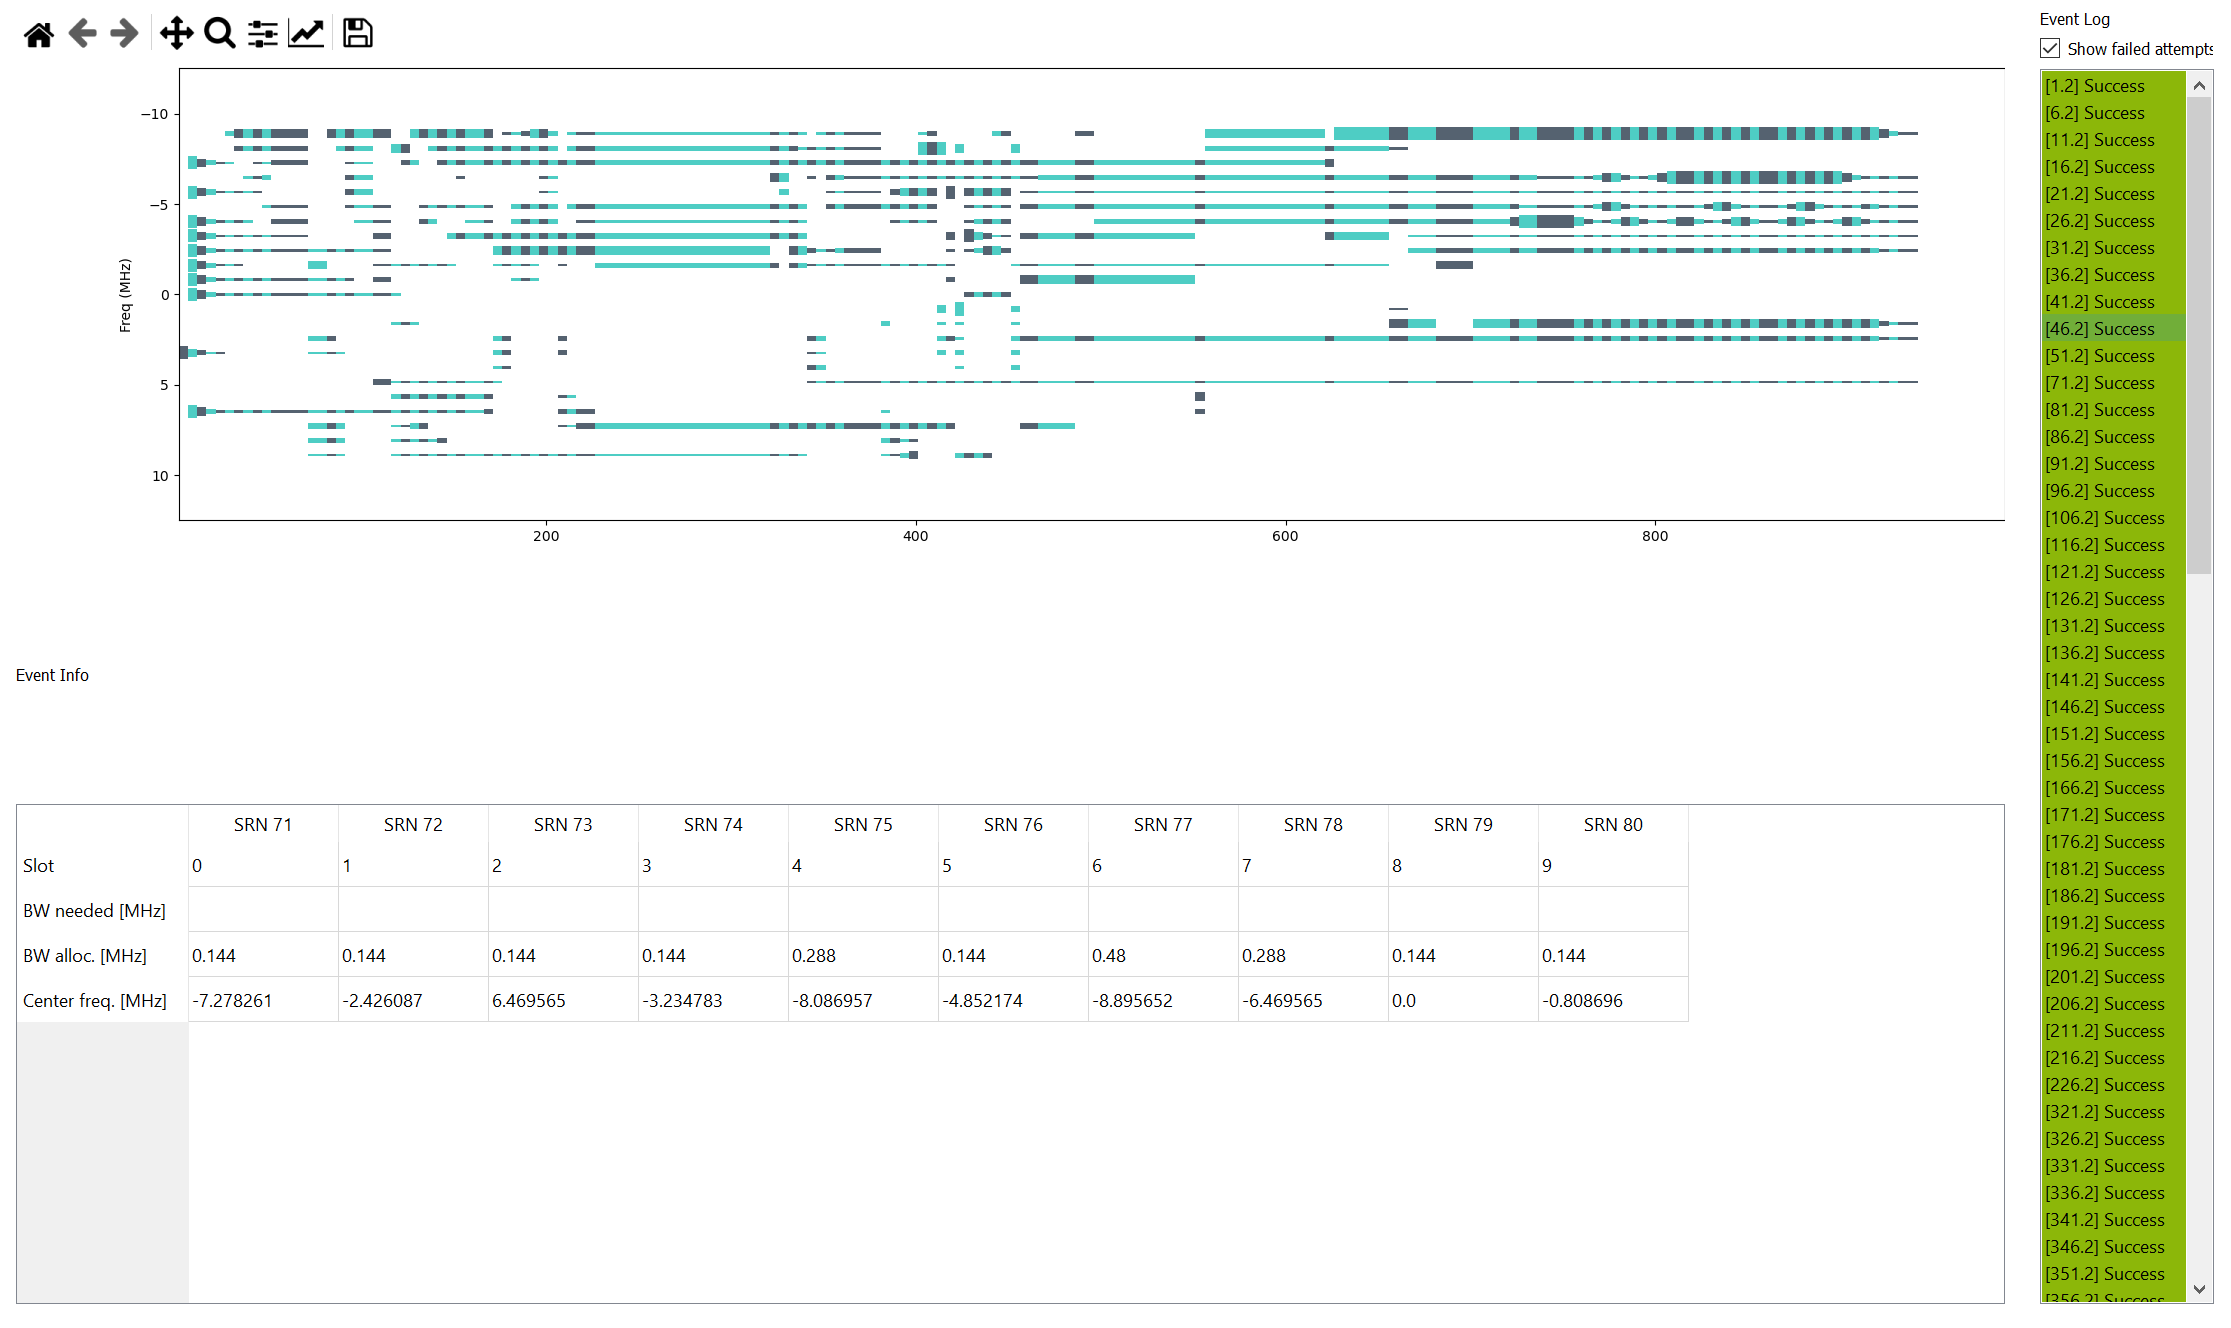
\includegraphics[width = 0.95\textwidth]{Alleys_Channel_Alloc.PNG}
    \caption{BW and channel allocations during the course of an SC$2$ Alleys of Austin scenario}
    \label{fig:16}
\end{figure}
\end{frame}
\begin{frame}{NET: Multi-hop Routing (1/4)}
    \footnotesize{\begin{itemize}
        \item RF propagation characteristics on a link changes during the course of an SC$2$ emulation due to: radio node mobility, physical obstacles, and terrain variations
        \item This leads to situations in which an SRN cannot directly communicate with another SRN in order to deliver its assigned flows: ``Node Blockages"
        \item An SRN $i$ declares a ``Node Blockage" w.r.t another relevant SRN $j$ in our network if it does not receive short control messages from SRN $j$ over the FSK control channel for a pre-specified period of time, i.e., $10$s
        \item A binary vector is constructed at each SRN indicating the link status between itself and another relevant SRN in our network$\longrightarrow$shared with other SRNs in our network over the FSK control channel
        \item An SRN uses these vectors from the other SRNs and along with its own vector, constructs a routing table$\longrightarrow$the SRN then applies the Dijkstra's algorithm over this routing table to route its assigned flows with minimal number of hops
    \end{itemize}}
\end{frame}
\begin{frame}{NET: Multi-hop Routing (2/4)}
\begin{figure}
    \centering
    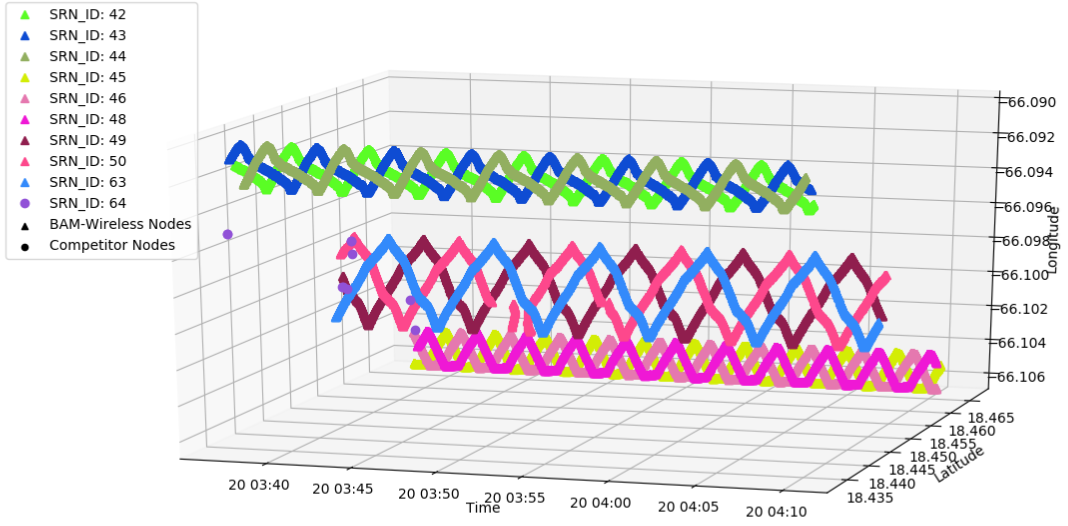
\includegraphics[width = 0.95\textwidth]{Payline_Node_GPS_Locations.PNG}
    \caption{SRN mobility as emulated in an SC$2$ Payline scenario causes variations in RF propagation characteristics}
    \label{fig:17}
\end{figure}
\end{frame}
\begin{frame}{NET: Multi-hop Routing (3/4)}
\begin{figure}
    \centering
    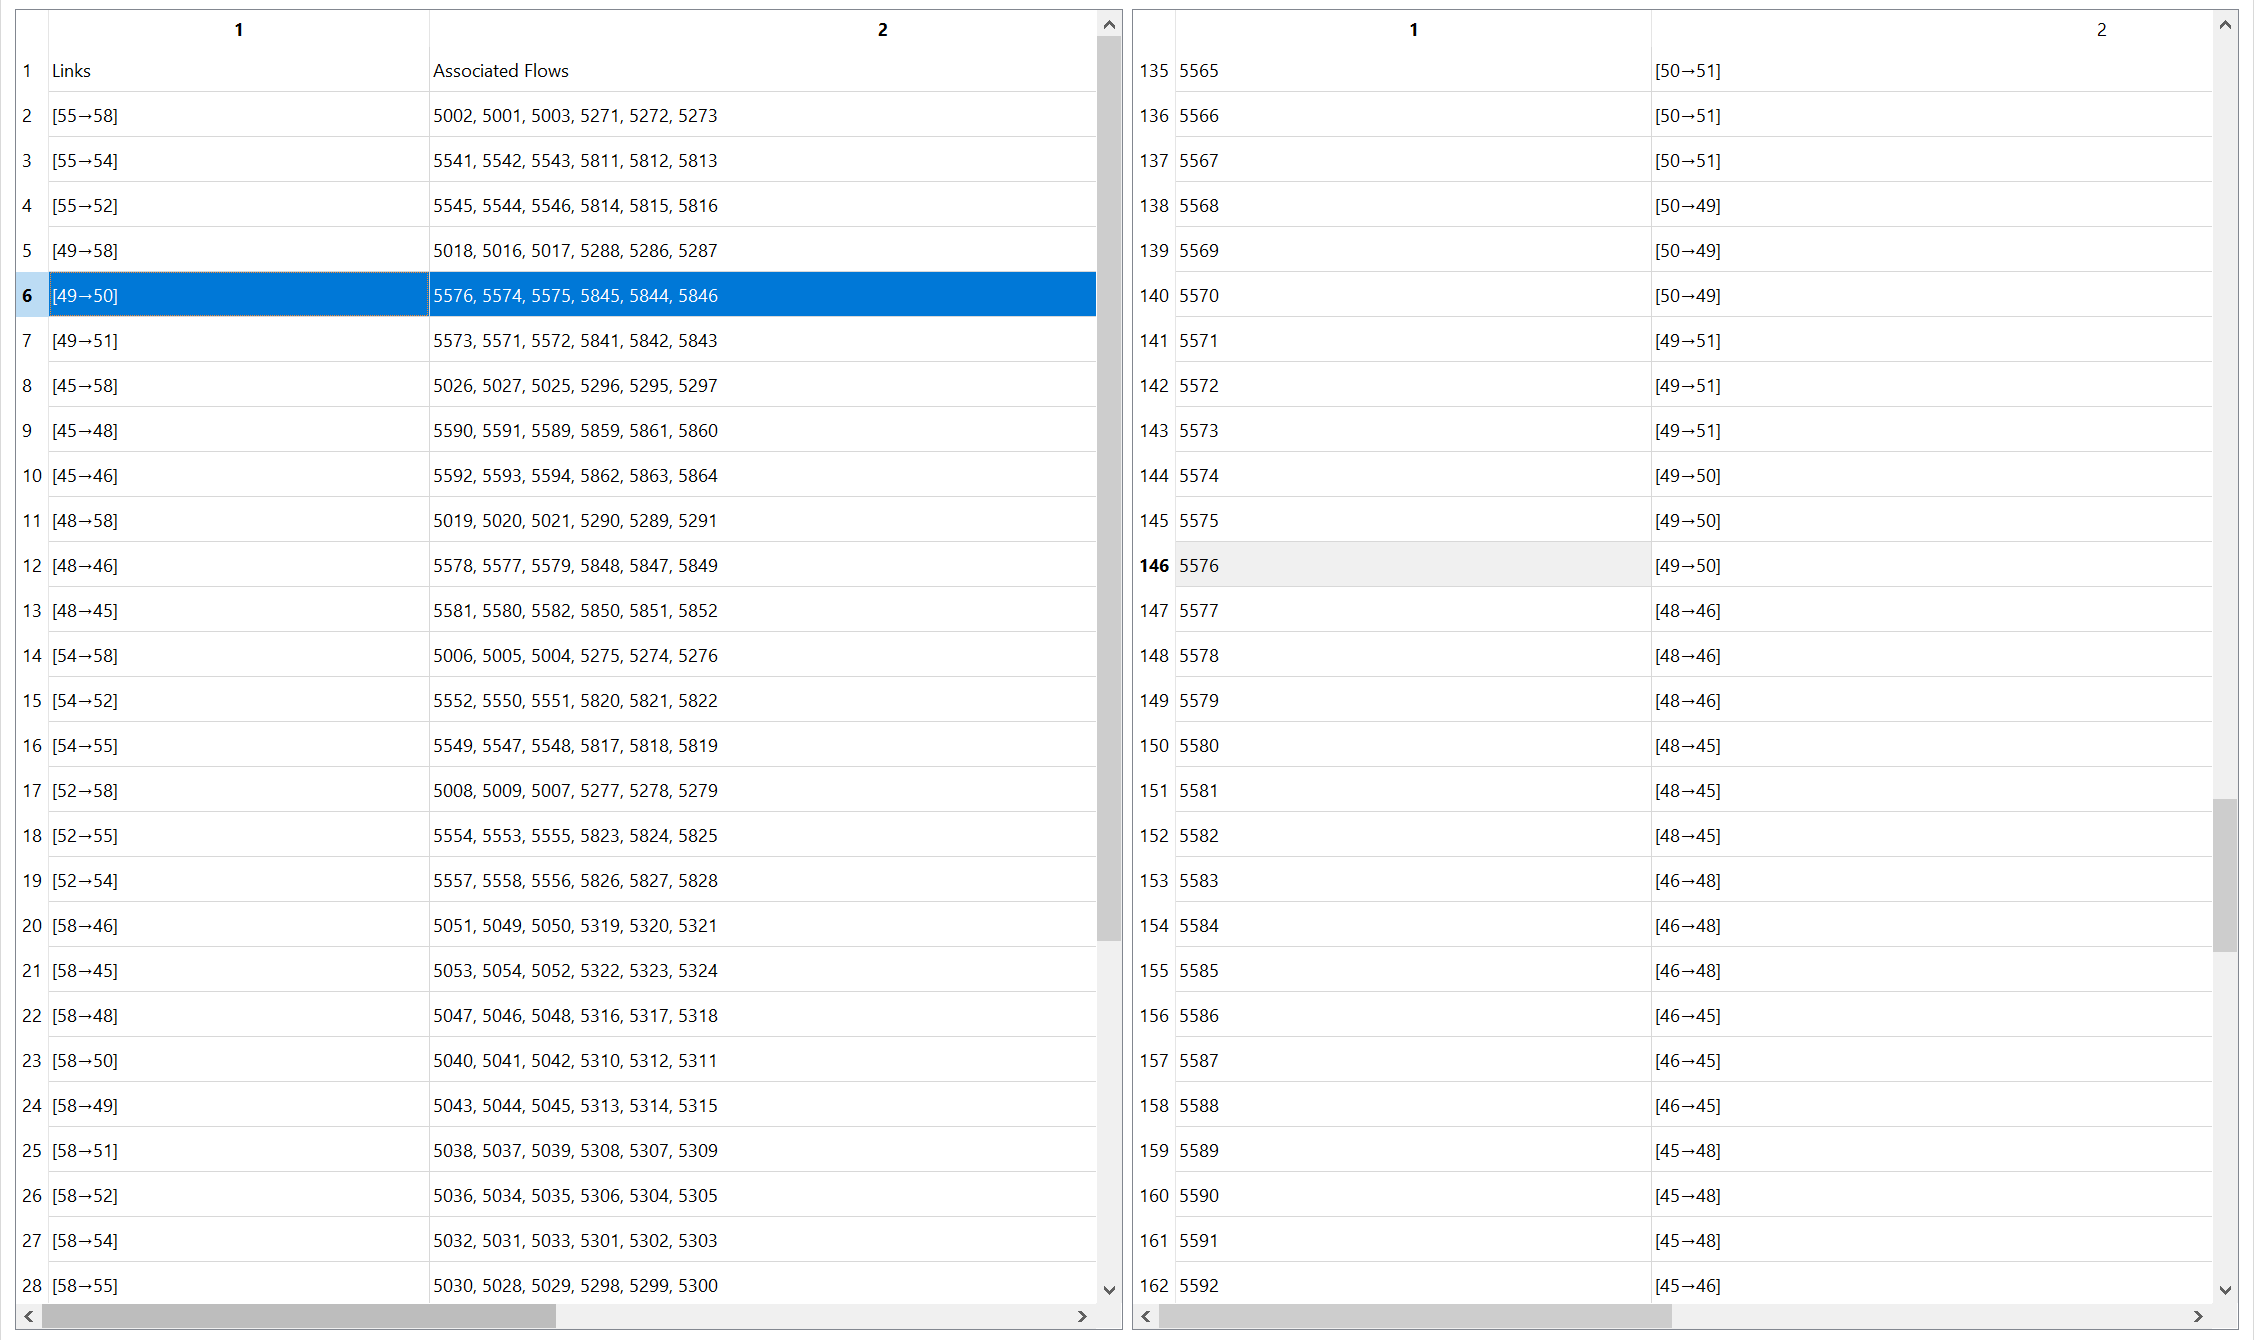
\includegraphics[width = 0.95\textwidth]{Link_Flow_Mapping.PNG}
    \caption{Link-Flow Mapping for our network in an SC$2$ Payline scenario}
    \label{fig:18}
\end{figure}
\end{frame}
\begin{frame}{NET: Multi-hop Routing (4/4)}
\begin{figure}
    \centering
    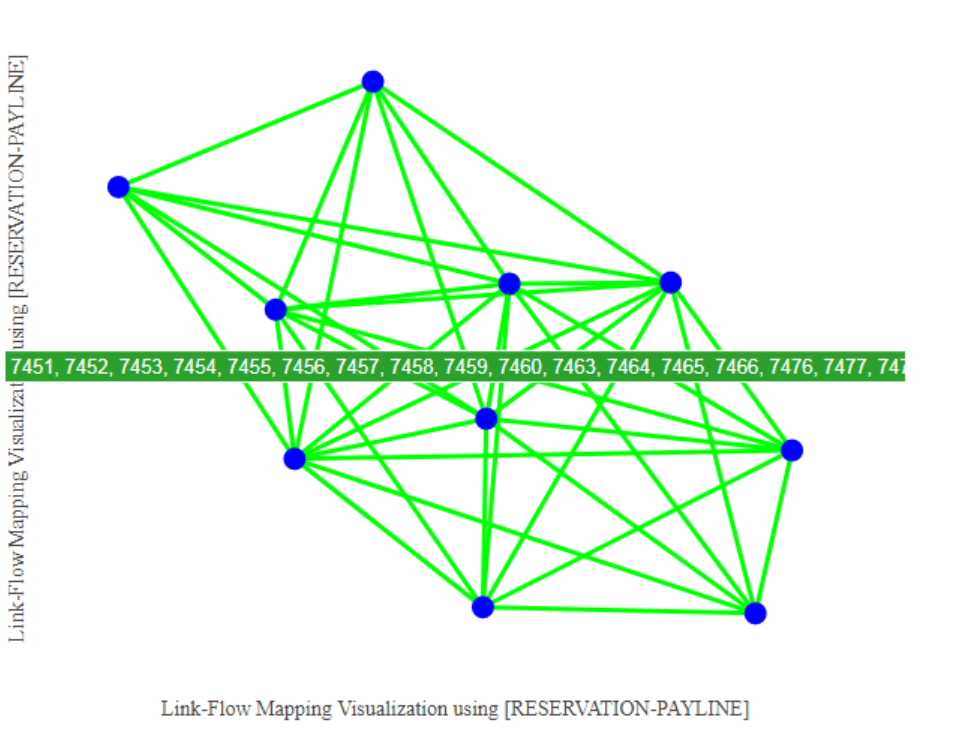
\includegraphics[width = 0.85\textwidth]{Network_Graph_Payline.PNG}
    \caption{Our network map in an SC$2$ Payline scenario}
    \label{fig:19}
\end{figure}
\end{frame}
\begin{frame}{BAM! Wireless Network Performance Analysis: SC$2$ Wildfire (1/10)}
    \footnotesize{\begin{itemize}
        \item Disaster relief deployment scenario: Wildfire in Lake Sutherland, WA
        \item $5$ stages of scenario emulation
        \item $5$ National Guard units deployed: each equipped with an Aerostat and $4$ unmanned water-bombers
        \item Stage $1$: the water-bombers get into position sending PLI information back to the Aerostat (pings)
        \item Stage $2{-}6$: $5$ water-bombers from $2$ teams ($3{+}2$) go out into the blaze to drop their load\texttt{-{}-}stream HD video back to the Aerostat ($15$ points per flow); remaining water-bombers loiter sending PLI information to the Aerostat ($1$ point per flow)
        \item Main idea: Collaborate in order to allow the ``deployed" water-bombers to use a significant portion of the spectrum for their high-priority flows
    \end{itemize}}
\end{frame}
\begin{frame}{BAM! Wireless Network Performance Analysis: SC$2$ Wildfire (2/10)}
\begin{figure}
    \centering
    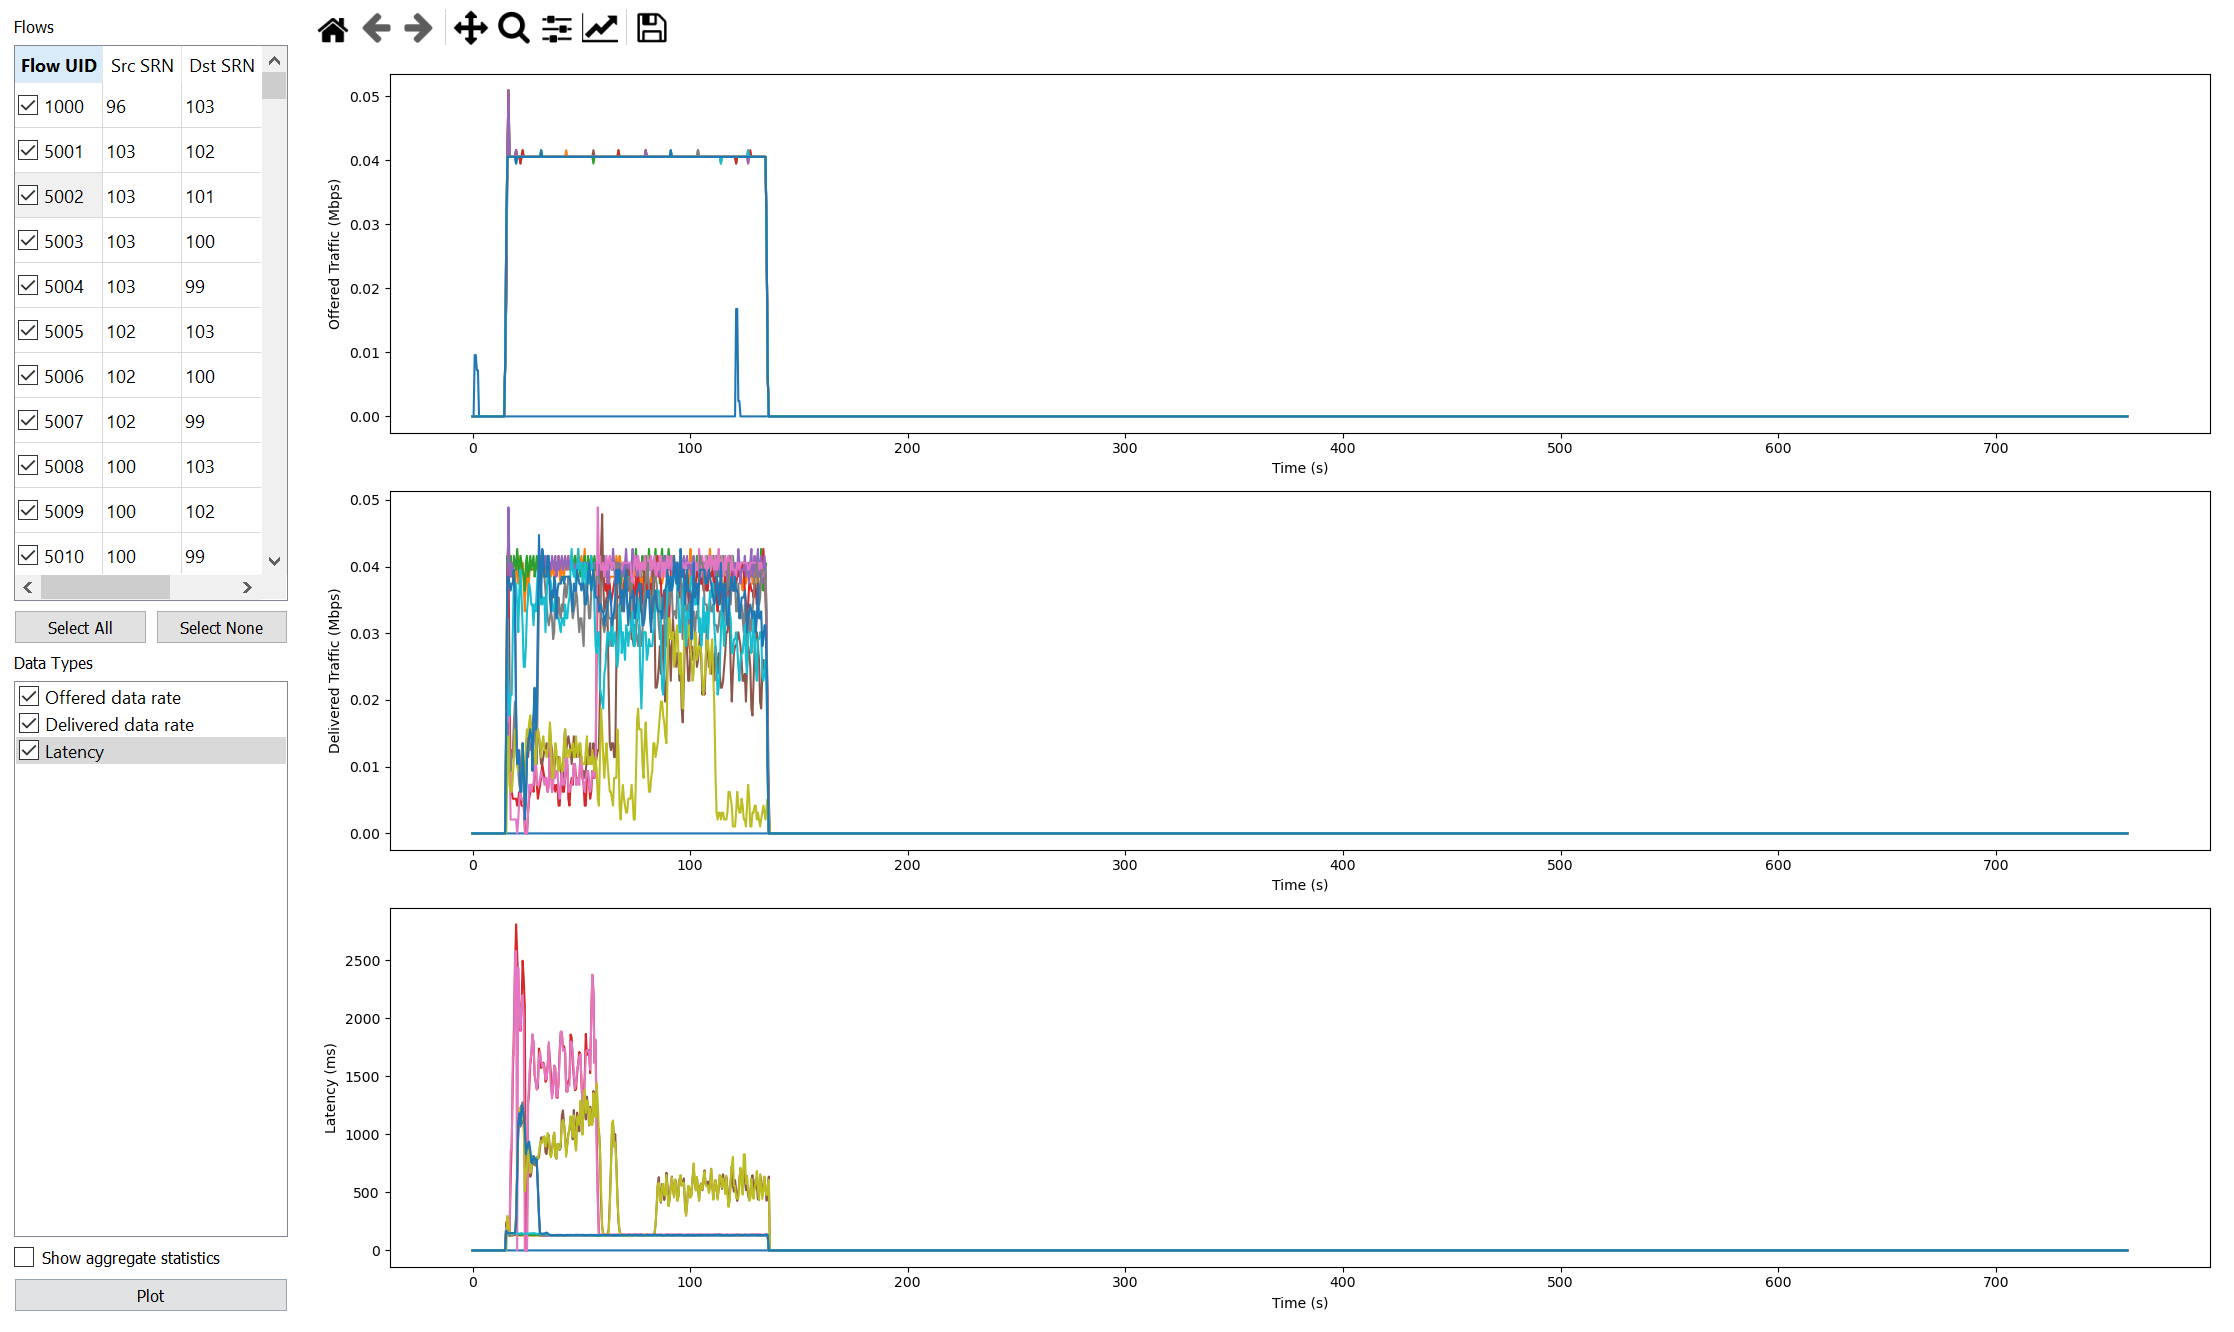
\includegraphics[width = 0.90\textwidth]{Wildfire_NET.PNG}
    \caption{The offered and delivered traffic statistics corresponding to the various selected links during Stage $1$ of an SC$2$ Wildfire scenario}
    \label{fig:20}
\end{figure}
\end{frame}
\begin{frame}{BAM! Wireless Network Performance Analysis: SC$2$ Wildfire (3/10)}
\begin{figure}
    \centering
    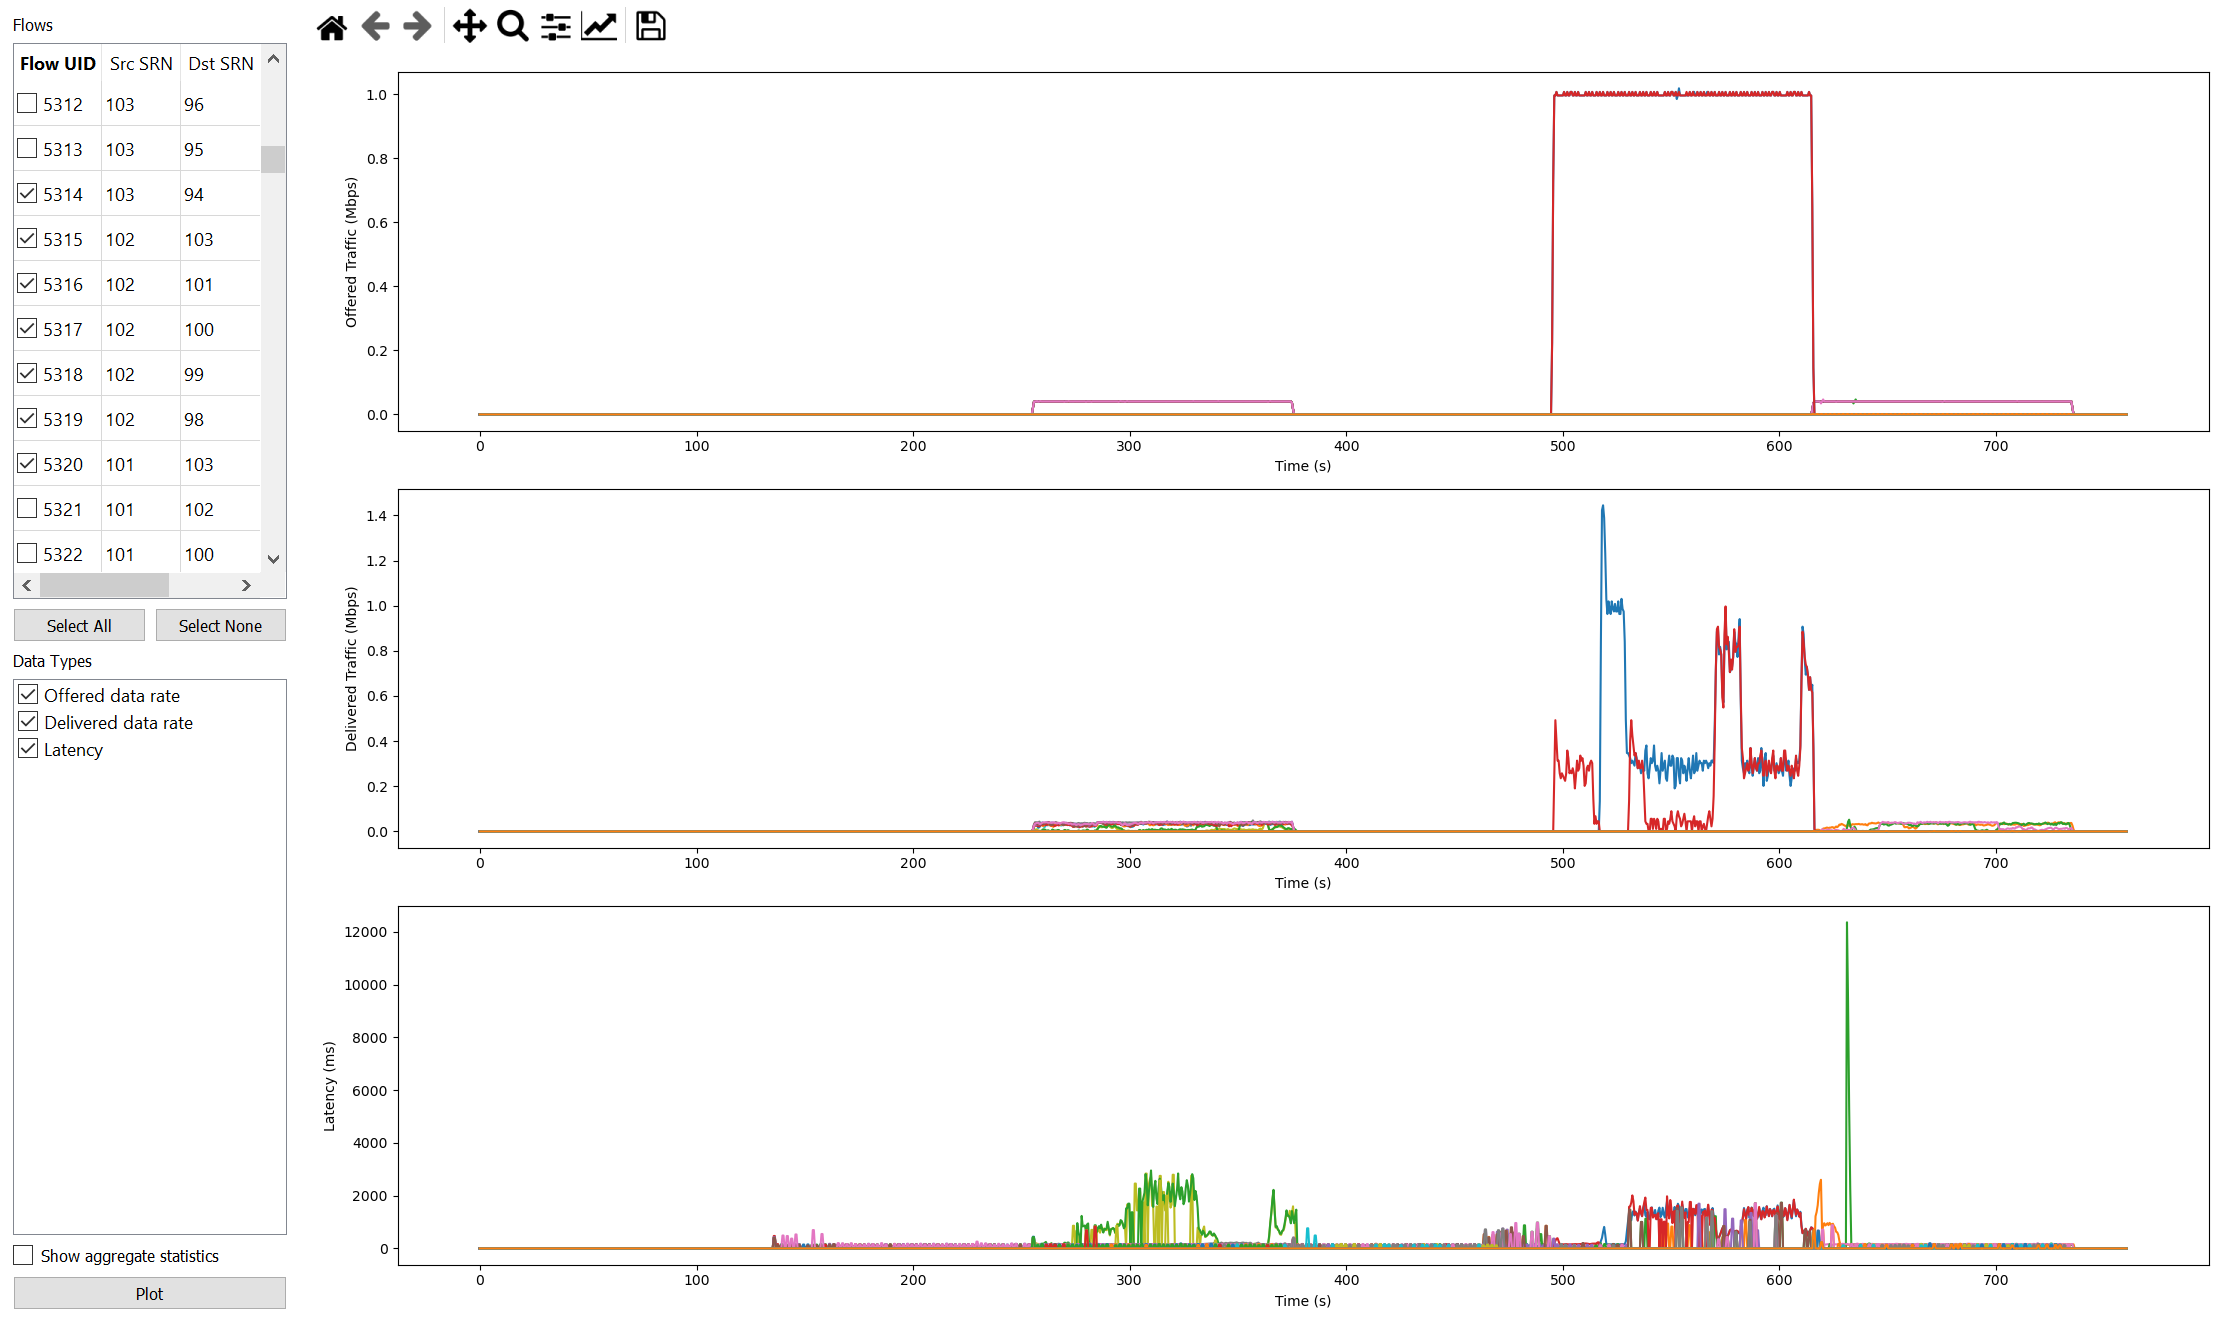
\includegraphics[width = 0.90\textwidth]{Wildfire_NET_2.PNG}
    \caption{The offered and delivered traffic statistics corresponding to the various selected links during Stage $5$ of an SC$2$ Wildfire scenario}
    \label{fig:21}
\end{figure}
\end{frame}
\begin{frame}{BAM! Wireless Network Performance Analysis: SC$2$ Wildfire (4/10)}
\begin{figure}
    \centering
    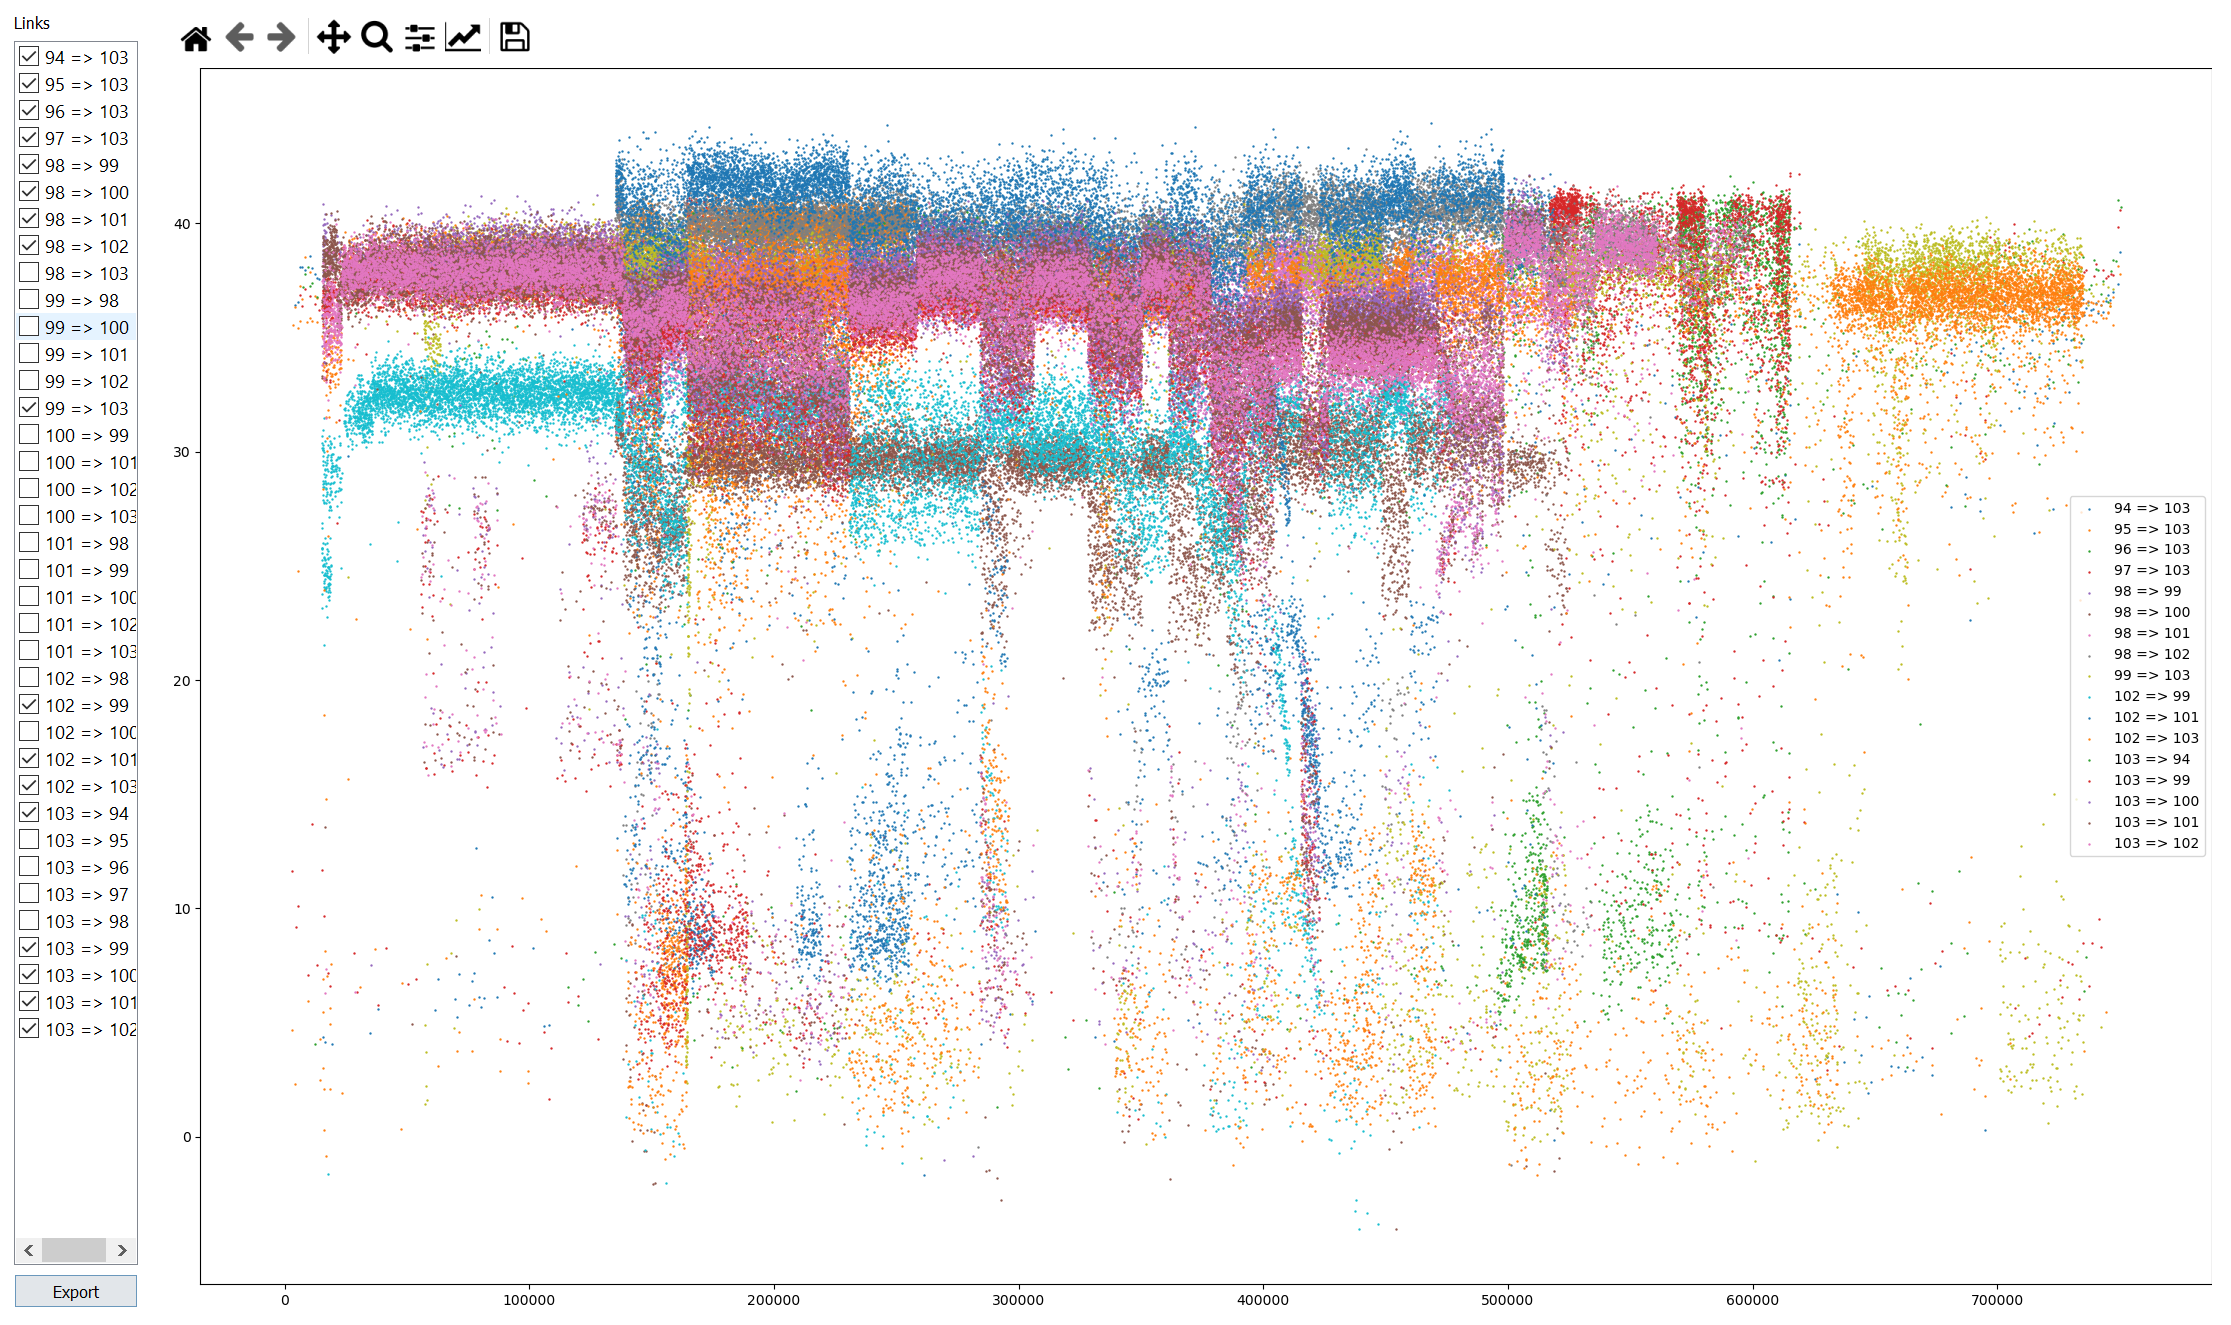
\includegraphics[width = 0.90\textwidth]{Wildfire_SNR.PNG}
    \caption{The estimated SNR on various selected links during an SC$2$ Wildfire scenario}
    \label{fig:22}
\end{figure}
\end{frame}
\begin{frame}{BAM! Wireless Network Performance Analysis: SC$2$ Wildfire (5/10)}
\begin{figure}
    \centering
    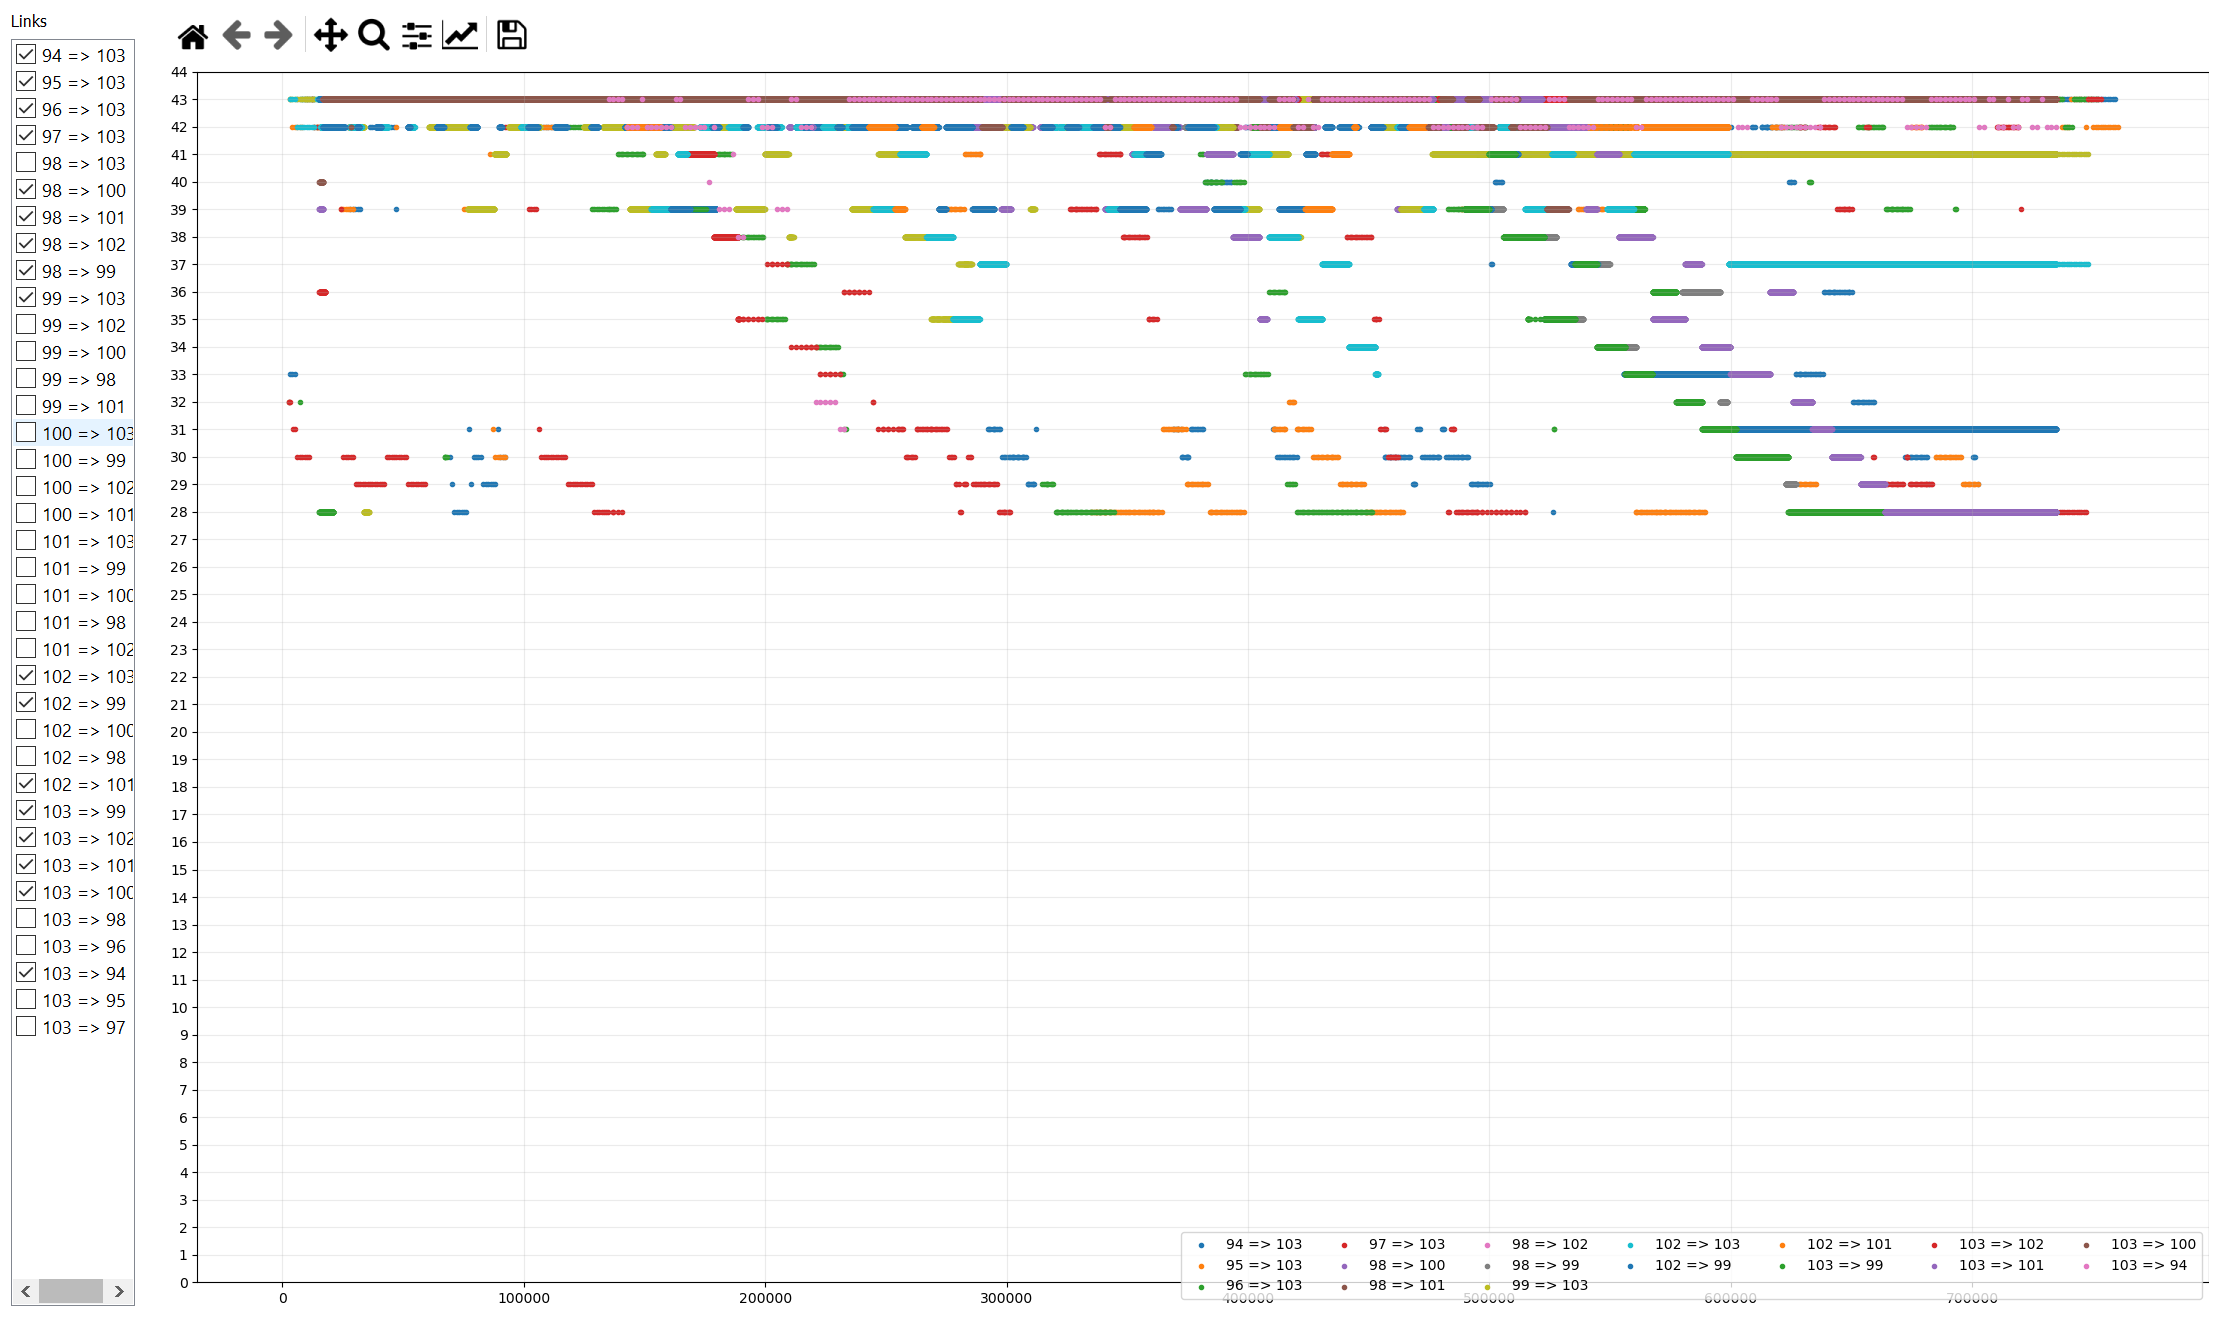
\includegraphics[width = 0.90\textwidth]{Wildfire_MCS.PNG}
    \caption{The MCS adaptation in response to changing estimated SNRs on the selected links, during an SC$2$ Wildfire scenario}
    \label{fig:23}
\end{figure}
\end{frame}
\begin{frame}{BAM! Wireless Network Performance Analysis: SC$2$ Wildfire (6/10)}
\begin{figure}
    \centering
    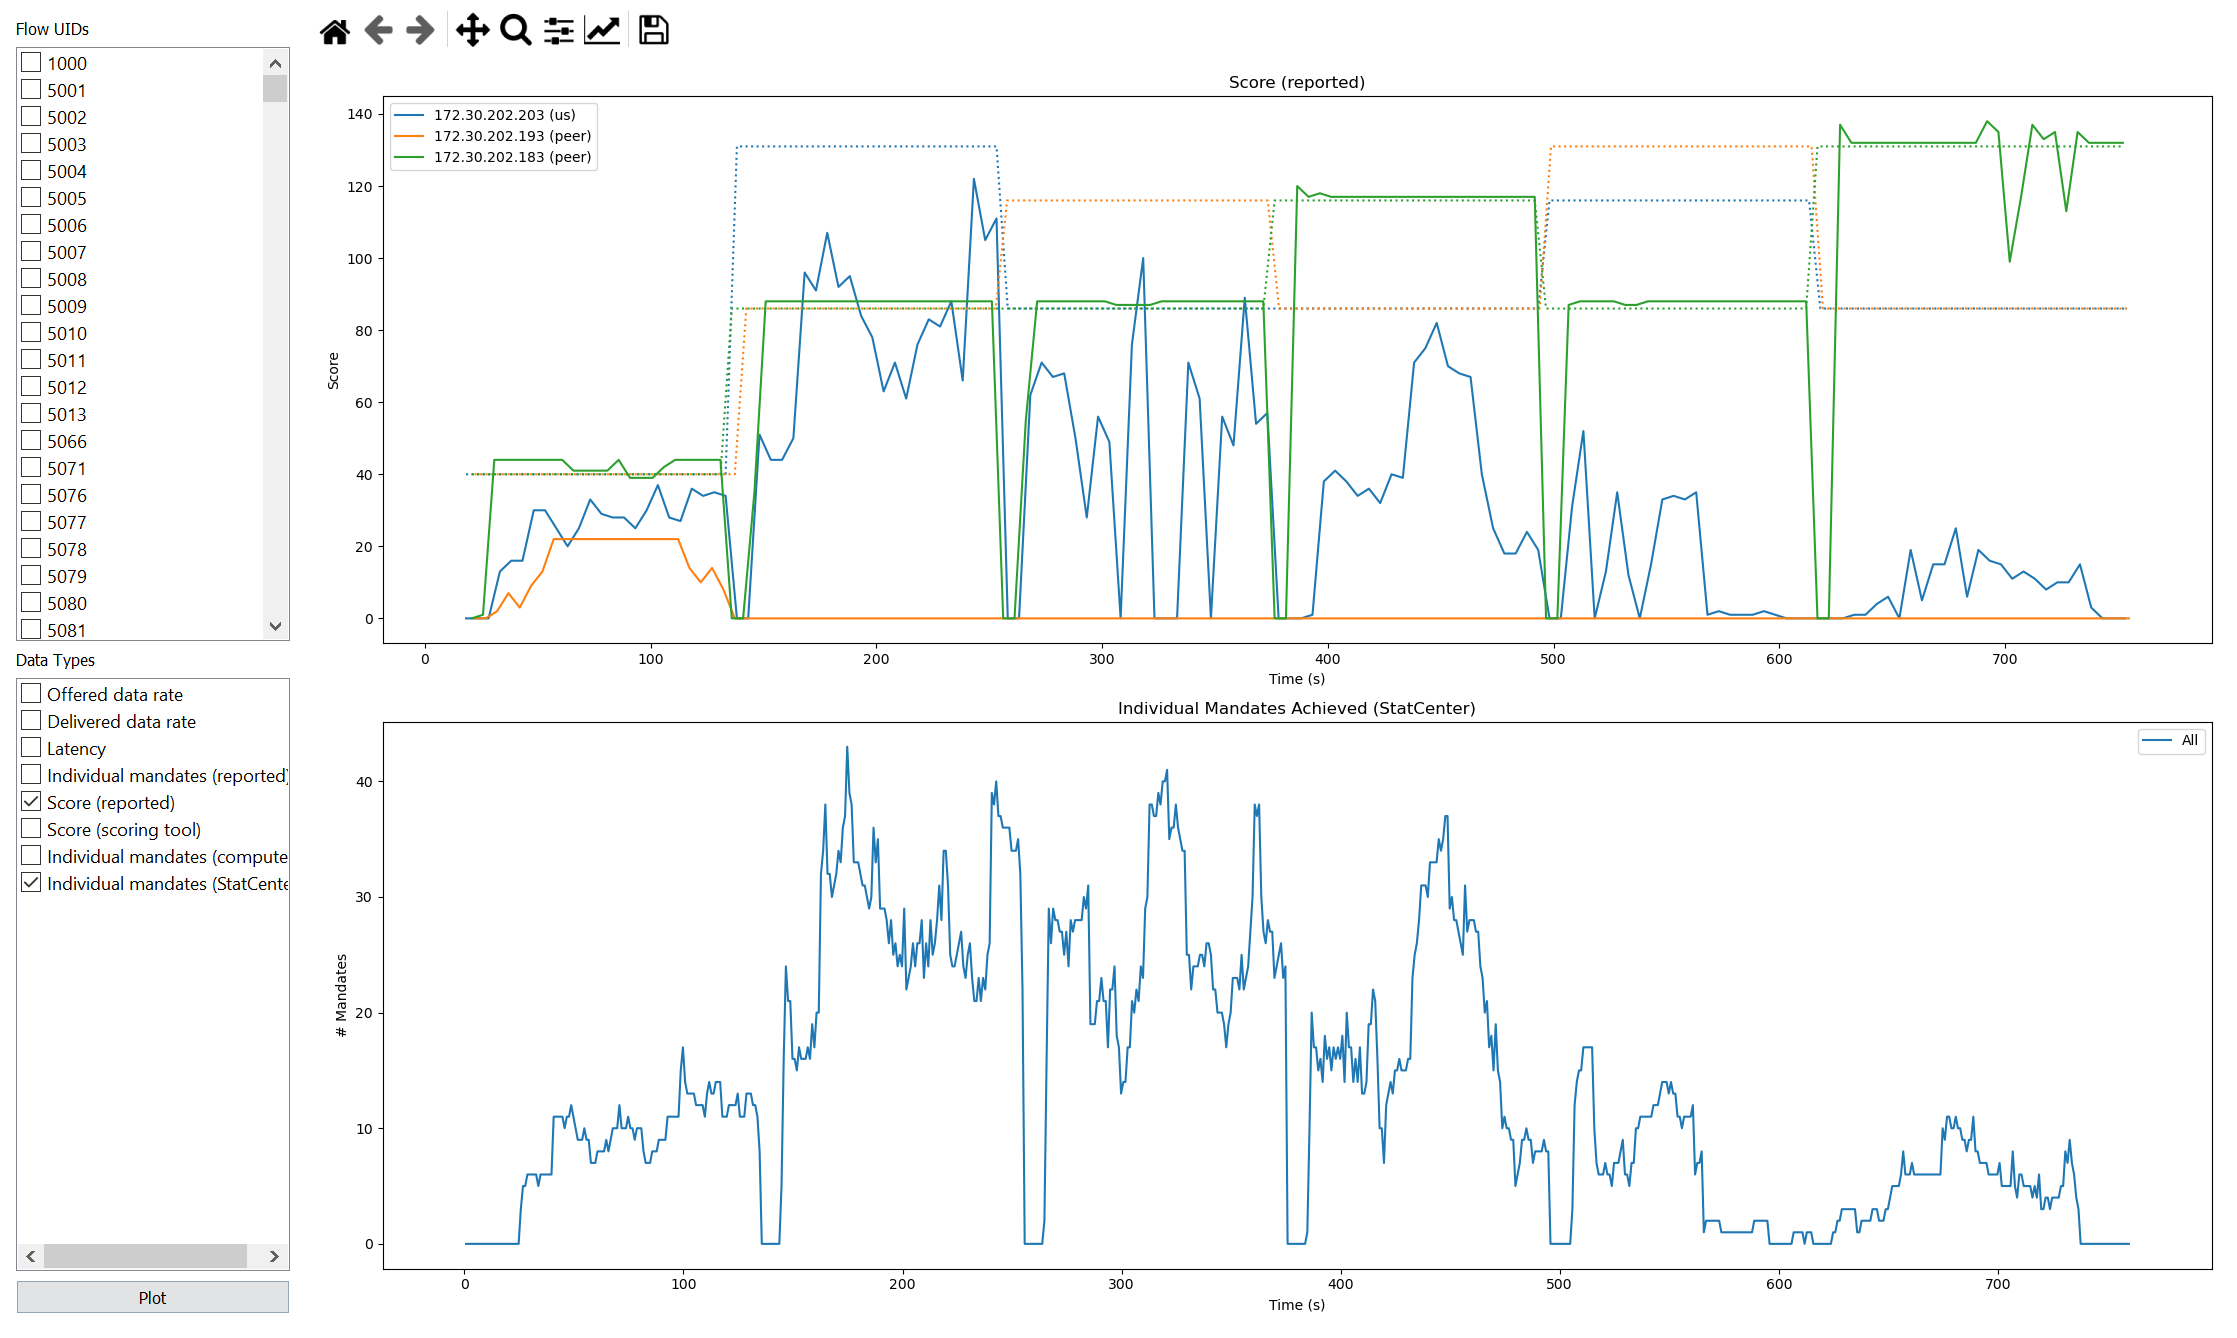
\includegraphics[width = 0.90\textwidth]{Wildfire_Scoring.PNG}
    \caption{The scores attained by our network and other competing networks during an SC$2$ Wildfire scenario, in addition to the number of QoS mandates satisfied by our network in a given time snapshot}
    \label{fig:24}
\end{figure}
\end{frame}
\begin{frame}{BAM! Wireless Network Performance Analysis: SC$2$ Wildfire (7/10)}
\begin{figure}
    \centering
    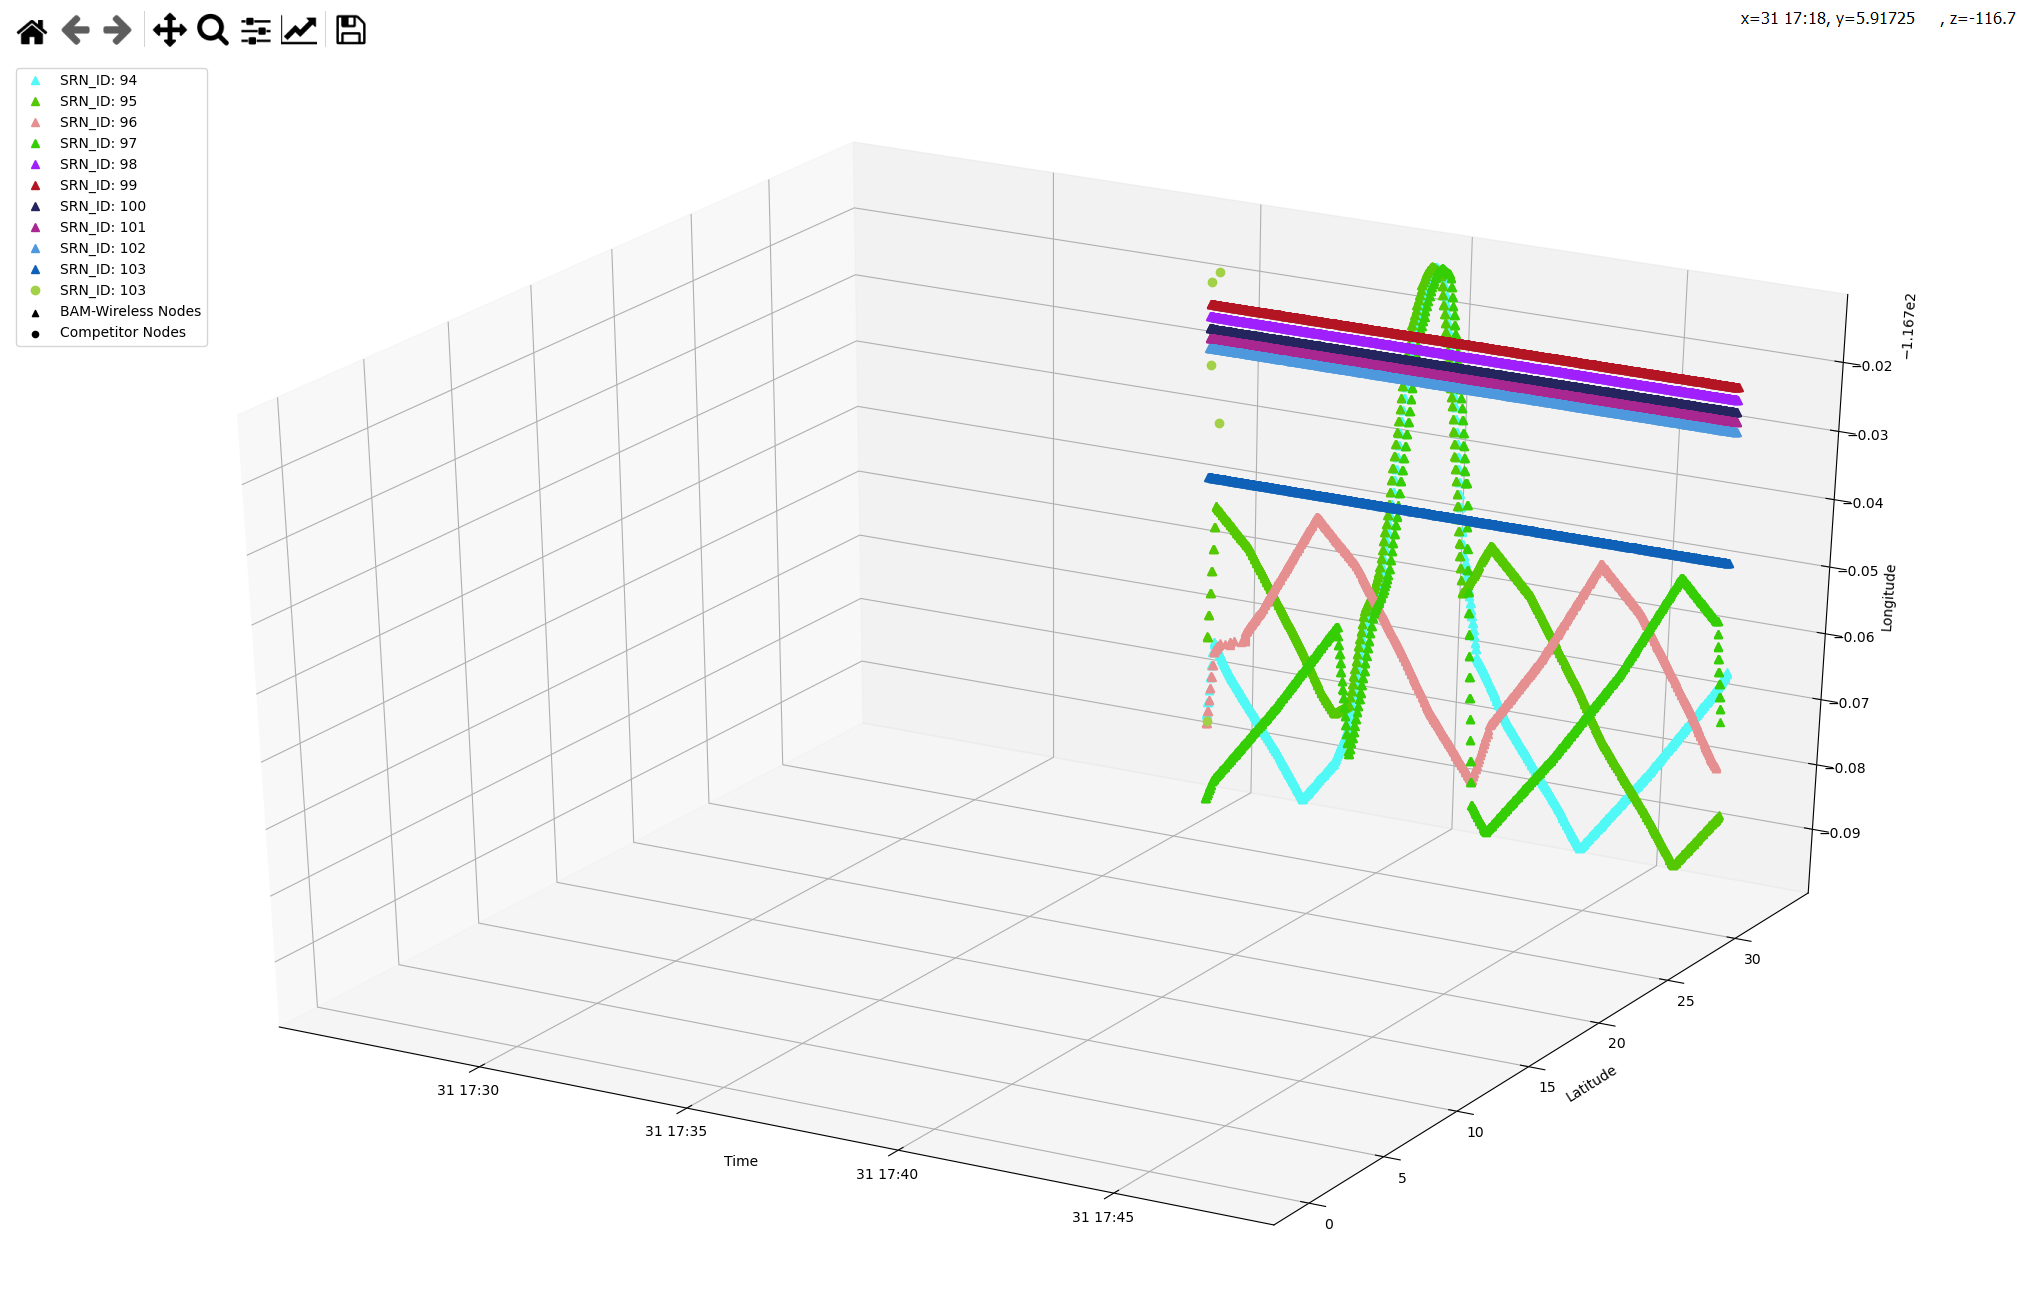
\includegraphics[width = 0.90\textwidth]{Wildfire_GPS.PNG}
    \caption{The reported GPS locations of our SRNs, in addition to those of our competing SRNs, during an SC$2$ Wildfire scenario}
    \label{fig:25}
\end{figure}
\end{frame}
\begin{frame}{BAM! Wireless Network Performance Analysis: SC$2$ Wildfire (8/10)}
\begin{figure}
    \centering
    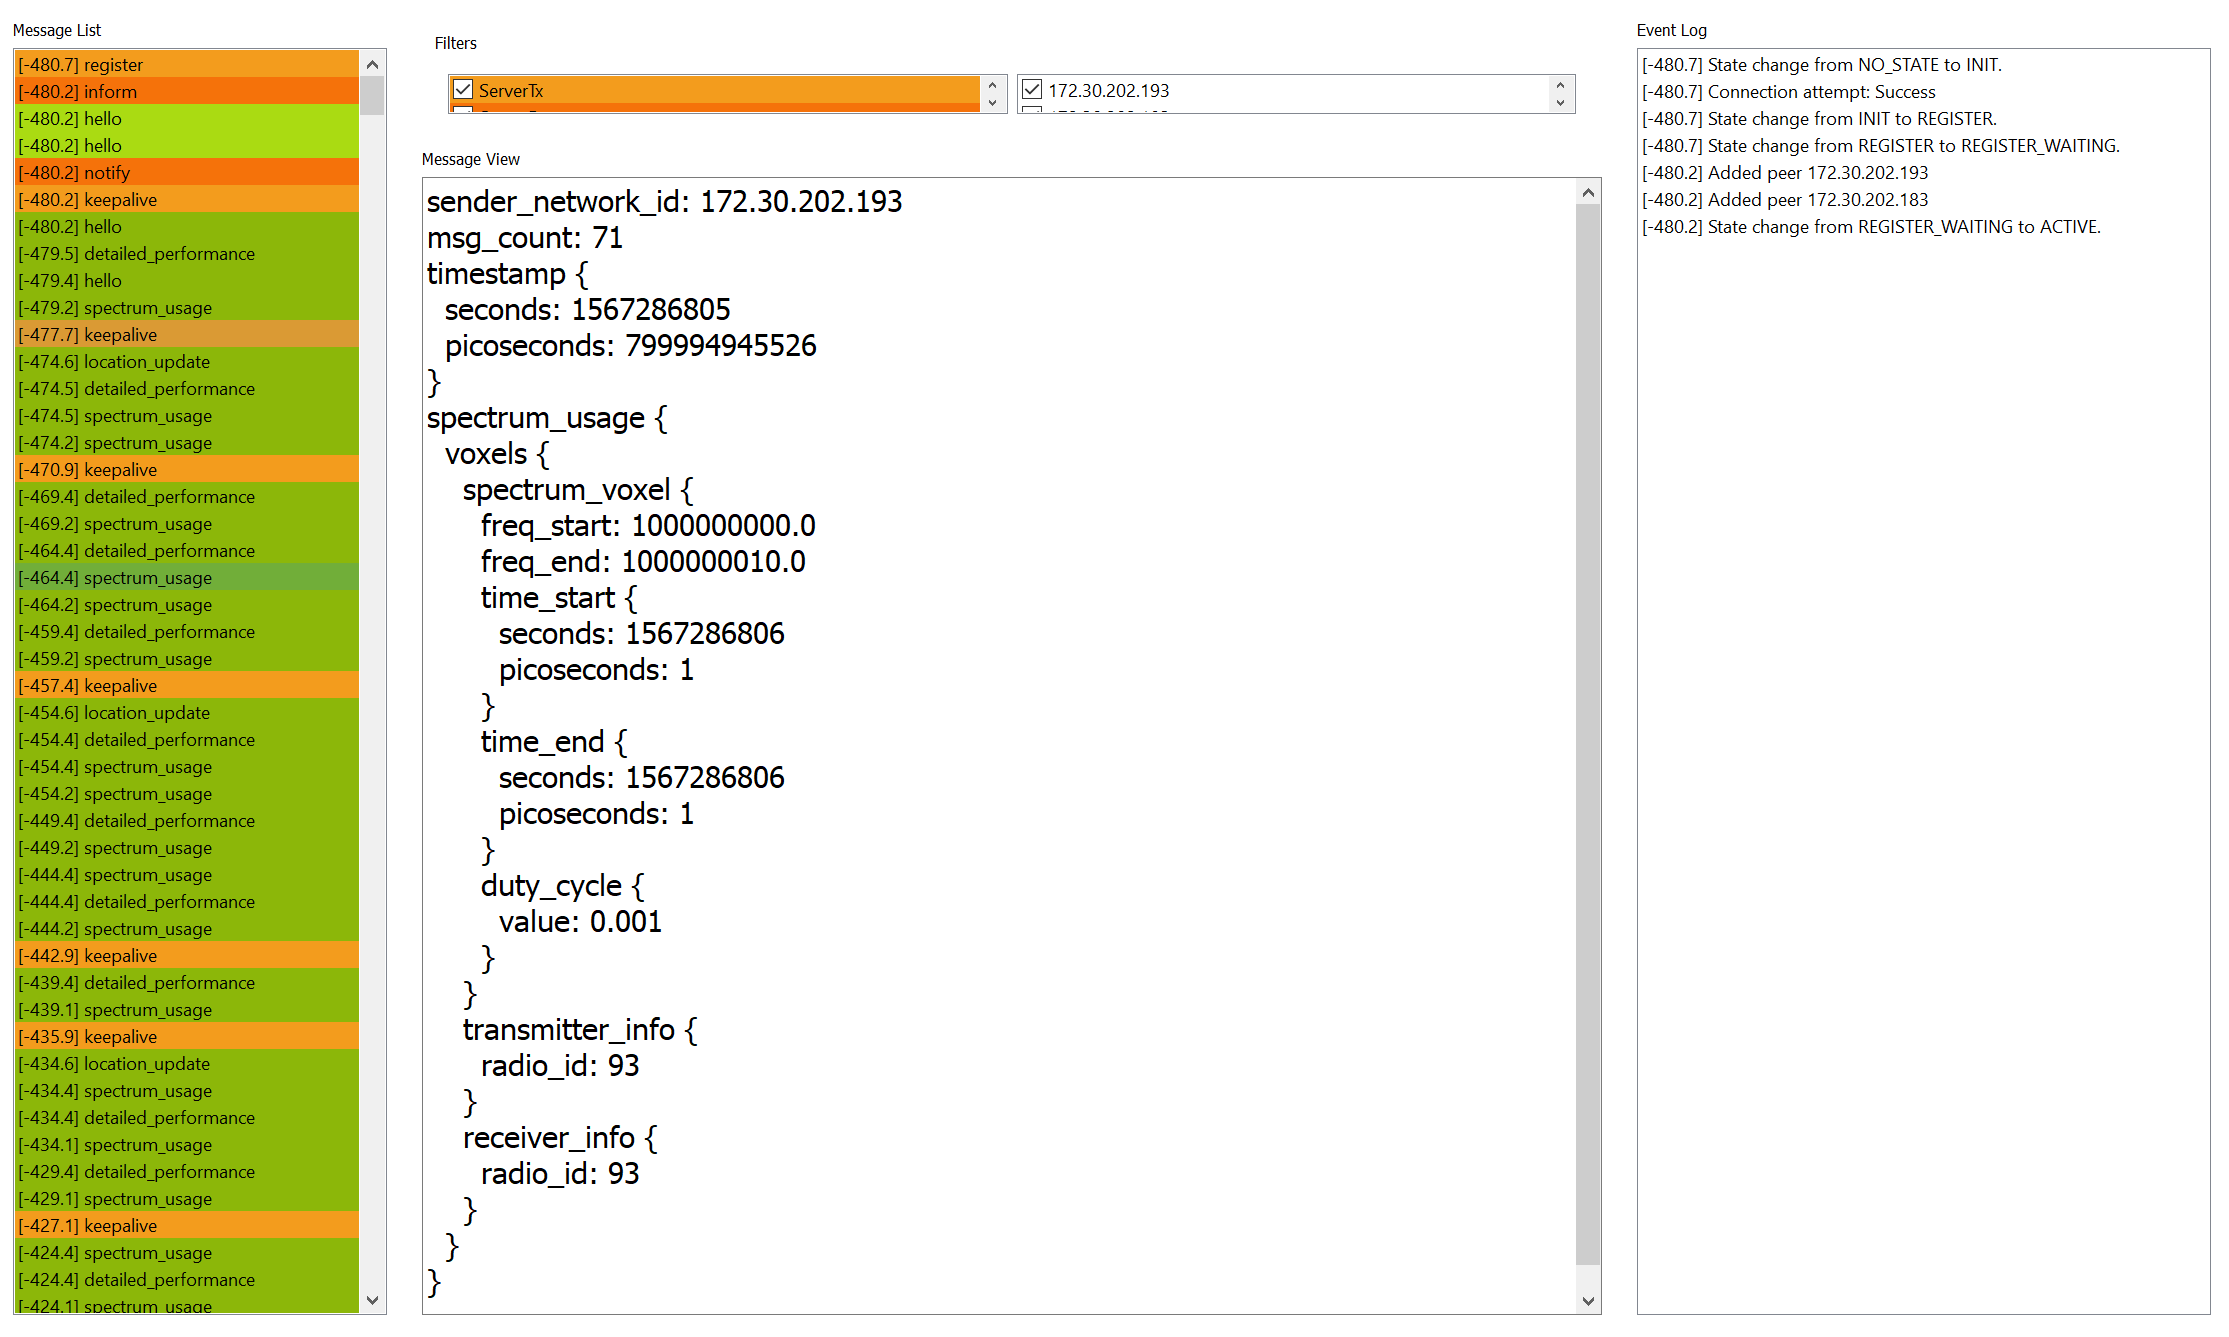
\includegraphics[width = 0.90\textwidth]{Wildfire_Collab.PNG}
    \caption{The description of various CIL message exchanges between our network and the collaboration server, in addition to those between our network and our peers, during an SC$2$ Wildfire scenario}
    \label{fig:26}
\end{figure}
\end{frame}
\begin{frame}{BAM! Wireless Network Performance Analysis: SC$2$ Wildfire (9/10)}
\begin{figure}
    \centering
    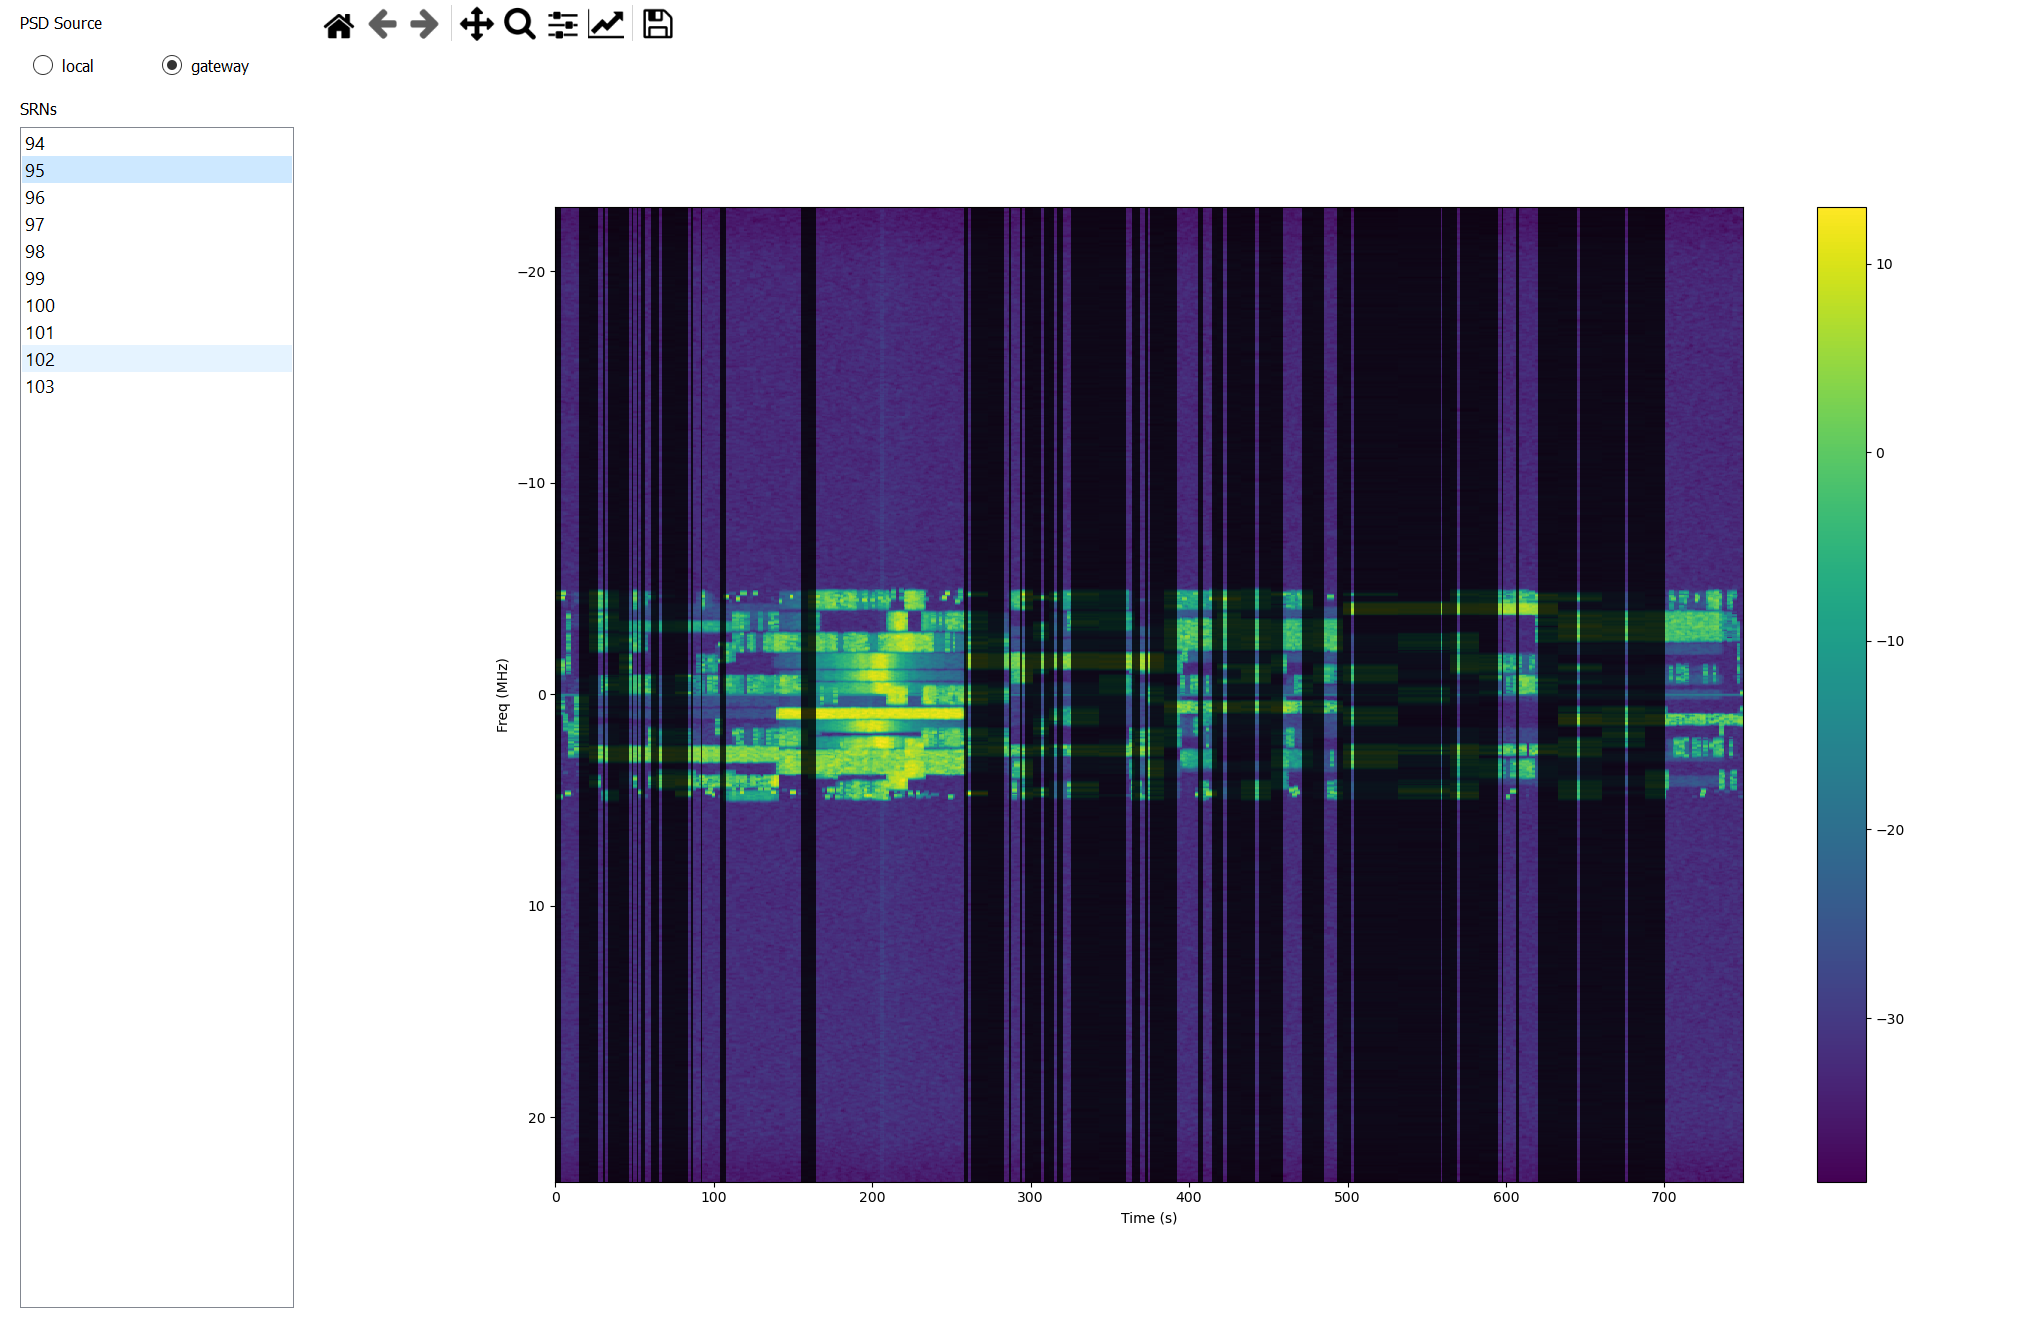
\includegraphics[width = 0.80\textwidth]{Wildfire_PSD.PNG}
    \caption{The PSD measurements received at our Gateway SRN from SRN $95$, in order to obtain location-specific spectrum occupancy information, during an SC$2$ Wildfire scenario}
    \label{fig:27}
\end{figure}
\end{frame}
\begin{frame}{BAM! Wireless Network Performance Analysis: SC$2$ Wildfire (10/10)}
\begin{figure}
    \centering
    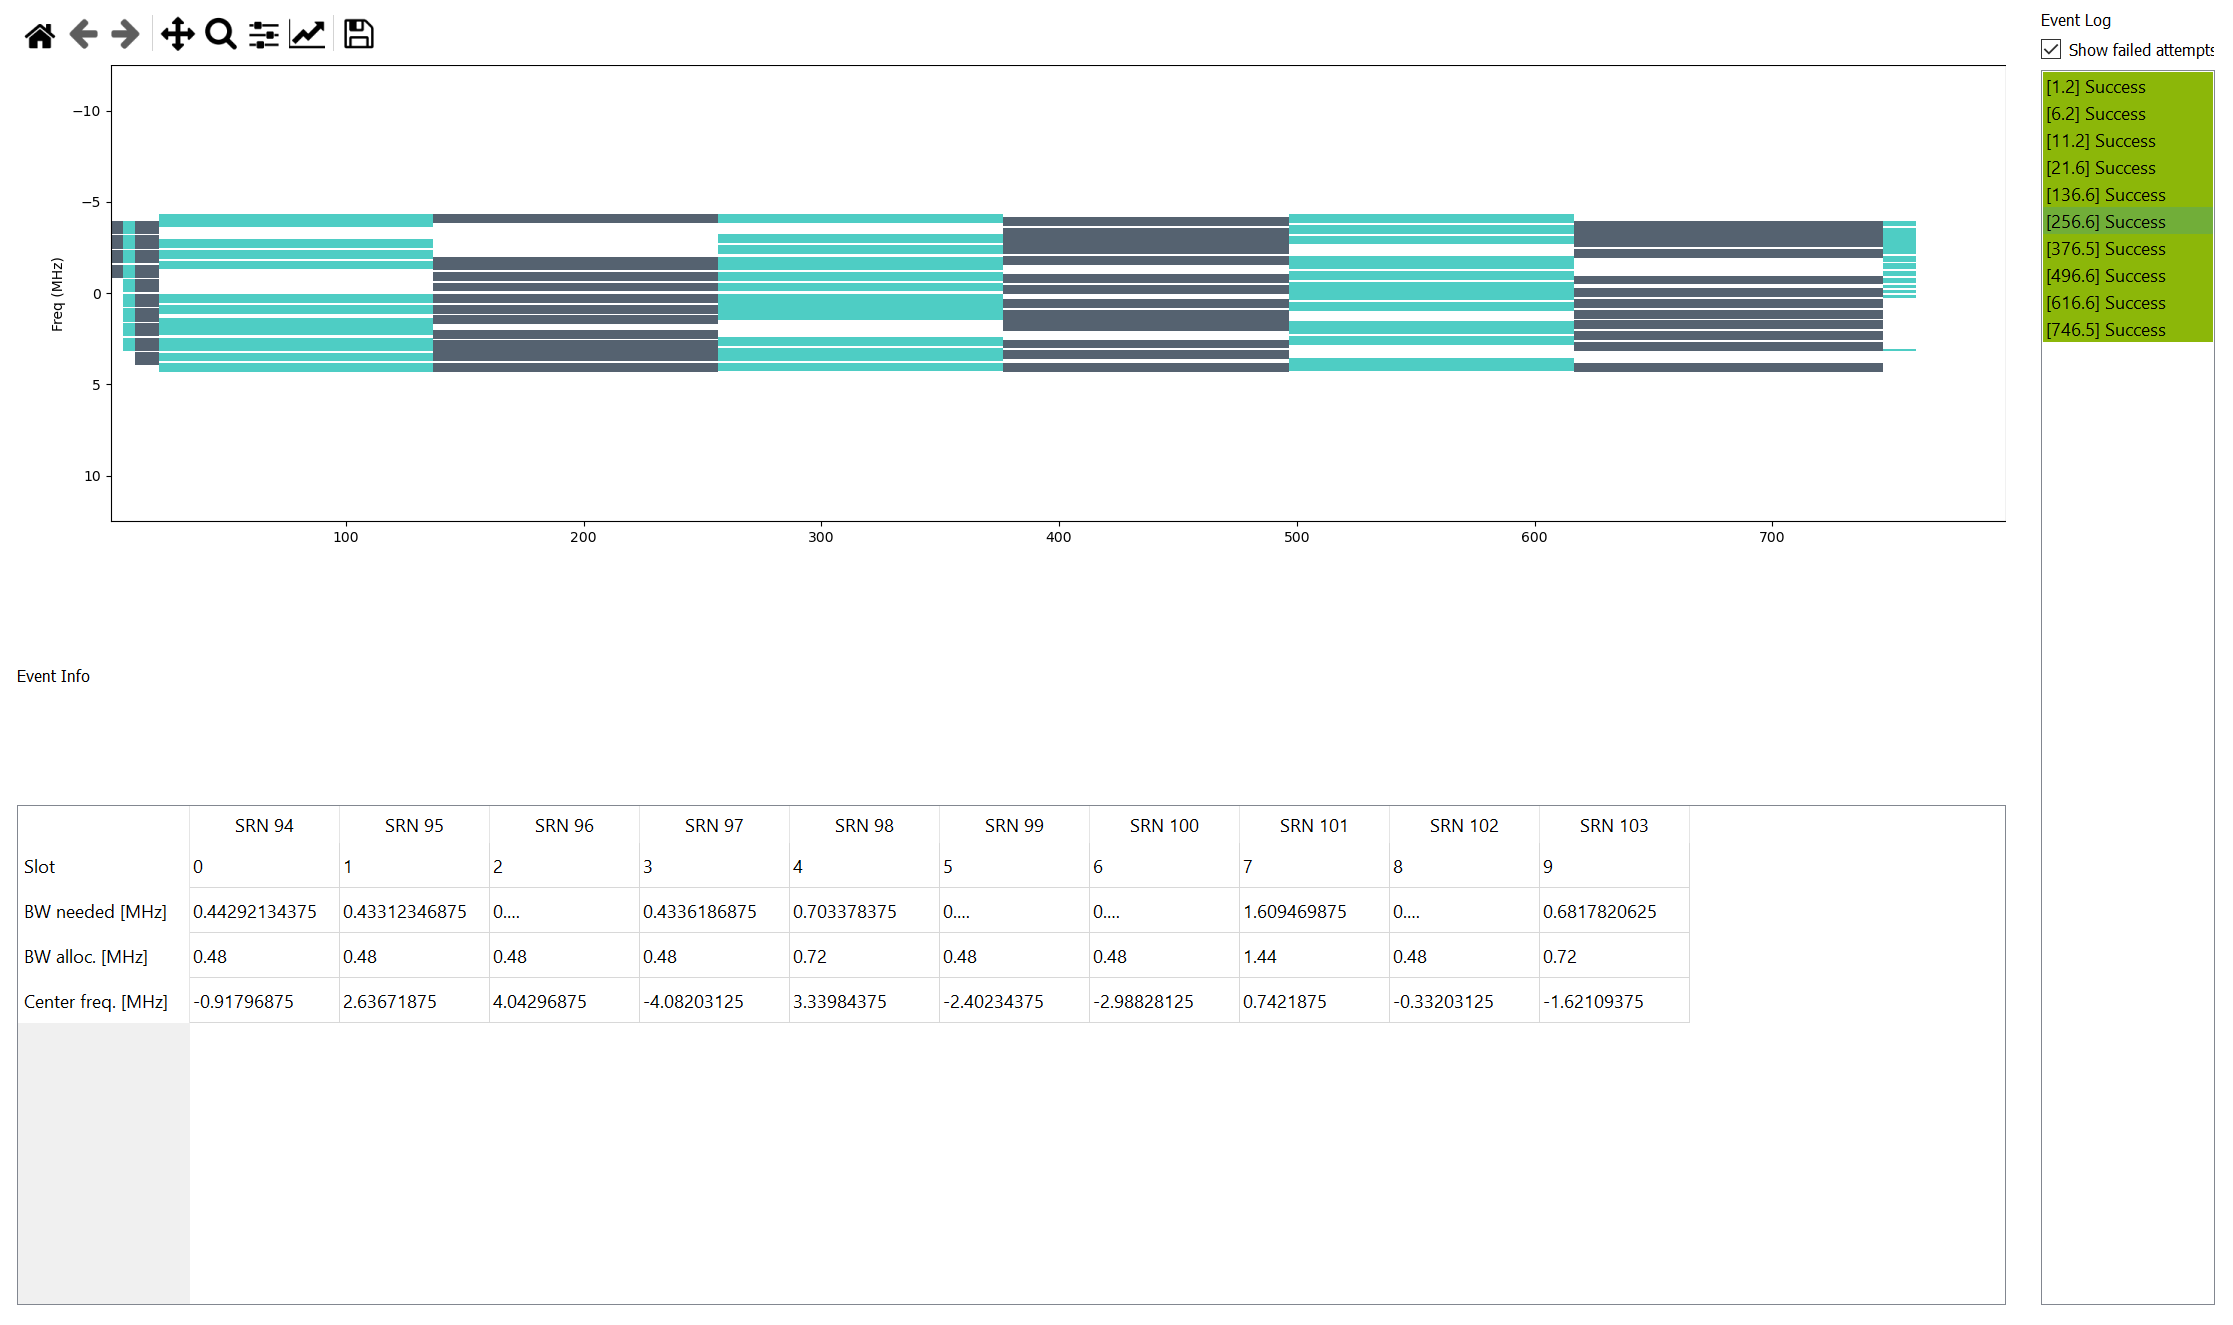
\includegraphics[width = 0.85\textwidth]{Wildfire_Channel_Alloc.PNG}
    \caption{The spectrum occupancy behavior of SRNs in our network (as guided by our GW) during an SC$2$ Wildfire scenario: allocations made based on link quality, traffic and QoS requirements, CIL messages, and PSD measurements}
    \label{fig:28}
\end{figure}
\end{frame}
\begin{frame}{}
  \centering \Huge
  \emph{Narrowing our focus\\
        \LARGE{Spectrum Sensing and Access in the MAC}}
\end{frame}
\begin{frame}{Signal Model}
    \footnotesize{\begin{itemize}
        \item $J{\geq}1$ PUs (licensed/priority/military users) and $1$ SU (cognitive radio)
        \item \[Y_k(i) = \sum_{j=1}^{J} H_{j,k}(i)X_{j,k}(i) + V_k(i),\]
        $k {\in} \{1,2,\dots,K\}$ is the frequency domain channel index;
        \\$X_{j,k}(i)$ is the signal of the $j$th PU in the frequency domain;
        \\$H_{j,k}(i)$ is the frequency domain channel between the $j$th PU and the SU; 
        \\$V_k(i) {\sim} \mathcal{CN}(0,\sigma_V^2)$ represents circularly symmetric additive complex Gaussian noise, i.i.d across frequency and time, and independent of $H$ and $X$
        \item OFDMA: $X_{j,k}(i)X_{g,k}(i){=}0, \forall j{\neq}g$;
        \\$j_{k,i}$ be the index of the PU that occupies the $k$th spectrum band at time $i$; \\$H_{k}(i){\triangleq}H_{j_{k,i},k}(i)$; 
        \\$X_{k}(i){\triangleq}X_{j_{k,i},k}(i)$ with $X_{k}(i){=}0$, if no PU is transmitting in the $k$th spectrum band at time $i$; Then,
        \[Y_k(i) = H_{k}(i)X_{k}(i) + V_k(i)\]
        \item Rayleigh fading channel: $H_k {\sim} \mathcal{CN}(0,\sigma_H^2)$, i.i.d. across frequency bands and time.
    \end{itemize}}
\end{frame}
\begin{frame}{PU Occupancy Model}
    \scriptsize{\begin{itemize}
        \item \[X_k(i) = \sqrt{P_{tx}}B_k(i)S_k(i),\]
        $P_{tx}$ is the transmission power of the PUs;
        \\$S_k(i)$ is the transmitted symbol modeled as a constant amplitude signal;
        \\$|S_k(i)|{=}1$, i.i.d. over time and across frequency bands;
        \\$B_k(i){\in}\{0,1\}$ is the binary spectrum occupancy variable;
        \item \[\vec{B}(i) = [B_1(i), B_2(i), B_3(i), \cdots, B_K(i)]^T {\in} \{0, 1\}^K\]
        \item PUs join and leave the spectrum at random times\texttt{-{}-}Temporal correlation: 
        \[\mathbb{P}(\vec{B}(i+1)|\vec{B}(j), \forall j \leq i) = \mathbb{P}(\vec{B}(i+1)|\vec{B}(i))\]
        \item The PUs occupy a number of adjacent spectrum bands, and vary their spectrum needs over time depending on time-varying traffic demands, channel conditions, etc.\texttt{-{}-}Frequency and Time correlation:
        \[\mathbb{P}(\vec{B}(i+1)|\vec{B}(i))=\mathbb{P}(B_{1}(i+1)|B_{1}(i))\prod_{k=2}^{K}\mathbb{P}(B_{k}(i+1)|B_{k}(i), B_{k-1}(i+1))\]
        \item Parameterized by $\vec{\theta}{=}[\vec{p}\ \vec{q}]^\intercal$; \\$\vec{p}{=}[p_{uv}{=}\mathbb{P}(B_{k}(i{+}1){=}1|B_{k{-}1}(i{+}1){=}u,B_{k}(i){=}v){:} u,v{\in}\{0,1\}]^{\intercal}$; \\$\vec{q}{=}[q_{w}{=}\mathbb{P}(B_{1}(i{+}1){=}1|B_{1}(i){=}w){:}w{\in}\{0,1\}]^\intercal$
    \end{itemize}}
\end{frame}
\begin{frame}{SU Spectrum Sensing Model}
    \begin{itemize}
        \item Owing to physical design limitations of its spectrum sensor\footnote{\tiny{S. Malecki, et. al., ``Energy and throughput efficient strategies...", 2011 IEEE 12th International Workshop on Signal Processing Advances in Wireless Communications}}, the SU can sense at most $\kappa$ out of $K$ spectrum bands at any given time, with $1{\leq}\kappa{\leq}K$
        \item HMM framework:
        \[\vec{Y}(i) = [Y_k(i)]_{k {\in} \mathcal K_i}\text{ is the observation vector};\]
        \[f(\vec{Y}(i)|\vec{B}(i), \mathcal K_i) = \prod_{k \in \mathcal K_i} f(Y_k(i)|B_k(i))\text{ is its PDF;}\]
        \[Y_k(i)|B_k(i) \sim \mathcal{CN}(0, \sigma_H^2P_{tx}B_k(i) + \sigma_V^2)\text{ from the signal model}\]
    \end{itemize}
\end{frame}
\begin{frame}{POMDP Agent Model (1/2)}
    \footnotesize{\begin{itemize}
        \item $5$-tuple: $(\mathcal B,\mathcal{A},\mathcal{Y},\mathbf{A},\mathbf{M})$
        \item The posterior belief:
        \begin{align*}
            \hat\beta_i(\vec{B}') &= \mathbb{P}(\vec{B}(i) = \vec{B}'|\vec{Y}(i), \mathcal K_i, \beta_i)\\&=
            \frac{\mathbb{P}(\vec{Y}(i)|\vec{B}', \mathcal{K}_i) \beta_i(\vec{B}')}{
            \sum_{\vec{B}'' {\in} \{0,1\}^K} \mathbb{P}(\vec{Y}(i)|\vec{B}'', \mathcal{K}_i) \beta_i(\vec{B}'')}.
        \end{align*}
        \item Given the posterior belief $\hat{\beta}_i$, we estimate $\vec{B}(i)$ as 
        $$
        \vec{\phi}(\hat{\beta}_{i})\triangleq \argmax_{\vec{B} {\in} \mathcal{B}} \hat{\beta}_{i}(\vec{B}),
        $$
        \item The reward function:
        \begin{equation}
            \nonumber
                R(\vec{B}(i), \hat{\beta}_i){=}\sum_{k=1}^{K} (1{-}B_k(i))(1{-}\phi_k(\hat{\beta}_{i})){-}\lambda B_k(i)(1 - \phi_k(\hat{\beta}_i))
        \end{equation}
        \item The prior belief in time-slot $i+1$:
        \[\beta_{i+1}(\vec{B}'')=\sum_{\vec{B}'}\mathbb{P}(\vec{B}(i+1) = \vec{B}''|\vec{B}(i)=\vec{B}')\hat{\beta}_{i}(\vec{B}')\]
    \end{itemize}}
\end{frame}
\begin{frame}{POMDP Agent Model (2/2)}
    \footnotesize{\begin{itemize}
        \item Goal: Find optimal spectrum sensing policy that maximizes the infinite-horizon discounted reward:
        \[\pi^{*}{=}\argmax_{\pi} V^{\pi}(\beta) \triangleq \mathbb{E}_{\pi} \Big[\sum_{i=1}^{\infty} \gamma^{i} R(\vec{B}(i), \hat{\beta}_i)|\beta_0 {=}\beta\Big]\]
        \item Re-formatting the formulation:
        \[\hat\beta_i{=}\hat{\mathbb B}(\beta_i, \mathcal K_i, \vec{Y}(i));\ \beta_{i+1}{=}{\mathbb B}(\hat\beta_i)\]
        \item $\pi^{*}$ is the solution to $V^*{=}\mathcal{H}[V^*]$, where the Bellman operator $V_{t+1}{=}\mathcal {H}[V_{t}]$ is
        \[V_{t+1}(\beta) = \max_{\mathcal{K} {\in} \mathcal{A}} \sum_{\vec{B} {\in} \mathcal{B}} \beta(\vec{B}) \mathbb{E}_{\vec{Y}|\vec{B}, \mathcal{K}} \Big[R(\vec{B}, \hat{\mathbb{B}}(\beta, \mathcal{K}, \vec{Y}))+\gamma V_{t}(\mathbb{B}(\hat{\mathbb{B}}(\beta, \mathcal{K}, \vec{Y})))\Big],\ \forall \beta\]
        \item This problem can be solved using value iteration methods. However, we face two challenges.
    \end{itemize}}
\end{frame}
\begin{frame}{POMDP Formulation: Two Challenges}
    \begin{itemize}
        \item \textcolor{red}{Challenge}: The parameter vector $\vec{\theta}$ is unknown, hence the belief updates $\hat{\mathbb B}$ and $\mathbb B$ cannot be computed;
        \\\textcolor{cyan}{Solution}: Estimate the transition model of the underlying MDP online\texttt{-{}-}concurrently with the POMDP optimal policy solver
        \item \textcolor{red}{Challenge}: The number of states of the underlying MDP scales exponentially with the number of spectrum bands, resulting in a high-dimensional belief space, hence, solving the Bellman optimality equation exactly is computationally infeasible;
        \\\textcolor{cyan}{Solution}: A randomized point-based approximate POMDP value iteration method known as \textcolor{magenta}{PERSEUS}
    \end{itemize}
\end{frame}
\begin{frame}{The Parameter Estimator\footnote{\tiny{W. Turin, ``Map decoding using the EM algorithm", 1999 IEEE 49th Vehicular Technology Conference}}}
    \begin{itemize}
        \item MLE problem:
        \[\vec{\theta}^{*} = \argmax_{\vec{\theta}} \log\Big(\sum_{\mathbf{B}} \mathbb{P}(\mathbf{B}, \mathbf{Y}| \vec{\theta})\Big)\]
        \item The Baum-Welch algorithm (EM for HMMs):
        \[\text{E-step: }Q(\vec{\theta}|\vec{\theta}^{(t)}) = \mathbb{E}_{\mathbf{B}|\mathbf{Y}, \vec{\theta}^{(t)}} \Big[ \log \Big(\mathbb{P}(\mathbf{B}, \mathbf{Y}|\vec{\theta}^{(t)})\Big)\Big]\]
        \[\text{M-step: }\vec{\theta}^{(t+1)} = \argmax_{\vec{\theta}} Q(\vec{\theta}|\vec{\theta}^{(t)})\]
    \end{itemize}
\end{frame}
\begin{frame}{PERSEUS\footnote{\tiny{T.J. Spaan, et. al., ``Perseus: Randomized Point-based Value Iteration for POMDPs", Journal of Artificial Intelligence Research, 2005}} (1/2)}
    \scriptsize{\begin{itemize}
        \item Leveraging the incumbent occupancy time-frequency correlation structure improves performance over independence assumptions\footnote{\tiny{S. Mosleh, et. al., ``Performance analysis of the Neyman-Pearson fusion center...", IEEE EUROCON 2009}}
        \item The POMDP agent randomly interacts with the environment to determine a set of so-called ``reachable beliefs" $\tilde{\mathcal{B}}$
        \item Goal: Improve the value of all the belief points in $\tilde{\mathcal{B}}$ by updating the value of only a subset of these belief points, chosen iteratively at random
        \item For finite-horizon POMDPs, $V^*$ can be approximated by a piece-wise linear and convex function
        \item The value function at iteration $t$ can be parameterized by a set of hyperplanes $\{\vec{\alpha}_{t}^{u}\}$, $u {\in} \{1,2,\dots,|\tilde{\mathcal{B}}|\}$, each representing a region of the belief space for which it is the maximizing element, and each associated with an optimal spectrum sensing action $\mathcal K_t^{u}$
        \item \[V_{t}(\beta) \approx \beta \cdot \vec{\alpha}_{t}^{u^*},\ u^* = \argmax_{u\in\{1,2,\dots,|\tilde{\mathcal{B}}|\}} \beta \cdot \vec{\alpha}_{t}^{u},\ \beta\cdot\vec{\alpha}{=}\sum_{\vec{B}}\beta(\vec{B})\vec{\alpha}(\vec{B})\]
        \item The set of hyperplanes $\{\vec{\alpha}_{t}^{u}\}$ associated with the set $\tilde{\mathcal{B}}$ are improved over multiple iterations of PERSEUS: given $\{\vec{\alpha}_{t}^{u}\}$ and the optimal spectrum sensing actions $\{\mathcal K_{t}^{u}\}$ at iteration $t$, a PERSEUS iteration generates a new set of hyperplanes $\{\vec{\alpha}_{t+1}^{u}\}$ and associated spectrum sensing actions $\{\mathcal K_{t+1}^{u}\}$
    \end{itemize}}
\end{frame}
\begin{frame}{PERSEUS (2/2)}
    \begin{itemize}
        \item \scriptsize{Initialization: $\tilde{\mathcal{U}}{=}\tilde{\mathcal{B}}$}
        \item \scriptsize{Backup: }
        \begin{itemize}
            \item \scriptsize{Find a new hyperplane associated with randomly chosen $\beta_{u}$:
            \[\vec{\alpha}_{t+1}^{u}=\Xi_{\mathcal K_{t+1}^{u}}^{u},\ \mathcal K_{t+1}^{u}=\argmax_{\mathcal{K} \in \mathcal{A}} \beta_u \cdot \Xi_{\mathcal{K}}^{u}\]
            \begin{align*}
                \Xi_{\mathcal{K}}^{u}(\vec{B}) = \mathbb{E}_{\vec{Y}|\vec{B}, \mathcal{K}} \Big[&R(\vec{B}, \hat{\mathbb{B}}(\beta_{u}, \mathcal{K}, \vec{Y}))+\\&\gamma \sum_{\vec{B}'}\mathbb{P}(\vec{B}(i+1){=} \vec{B}'|\vec{B}(i){=}\vec{B})\Xi_{\mathcal{K}, \vec{Y}}^{u}(\vec{B}')\Big]
            \end{align*}
            \[\Xi_{\mathcal{K}, \vec{Y}}^{u}=\argmax_{\alpha_{t}^{u'}, u' {\in} \{1, 2, \dots, |\tilde{\mathcal{B}}|\}} \mathbb{B}(\hat{\mathbb{B}}(\beta_{u}, \mathcal{K}, \vec{Y}))\cdot\alpha_{t}^{u'}\]}
            \item \scriptsize{Backup comparison: If $\beta_{u}{\cdot}\vec{\alpha}_{t+1}^{u}{\geq}V_{t}(\beta_{u})$, the newly defined hyperplane generates an improved value function; otherwise ($\beta_{u}{\cdot}\vec{\alpha}_{t+1}^{u}{<}V_{t}(\beta_{u})$), the value function is worsened and the previous hyperplane is kept, hence $\vec{\alpha}_{t+1}^{u}{:=}\vec{\alpha}_{t}^{u}$ and $\mathcal K_{t+1}^{u}{:=}\mathcal K_{t}^{u}$
            \item Backup extension (to other beliefs in $\tilde{U}$): 
            $$
                \tilde{\mathcal{U}}\leftarrow \tilde{\mathcal{U}}\setminus\{\beta_u\}\setminus
                \{\beta'\in\tilde{\mathcal{U}}:\beta'{\cdot}\vec{\alpha}_{t+1}^{u}\geq V_t(\beta')\}
            $$}
            \item \scriptsize{Backup termination: $\tilde{U}{=}\phi$}
        \end{itemize}
        \item \scriptsize{Termination: $|V_{t{+}1}(\beta){-}V_{t}(\beta)|{<}\epsilon,\ \forall \beta{\in} \tilde{\mathcal{B}},\ \epsilon{>}0$}
    \end{itemize}
\end{frame}
\begin{frame}{PERSEUS Heuristics}
    \begin{itemize}
        \item \textcolor{cyan}{Fragmentation}: smaller, independent sets of correlated channels governed by incumbent-specific behavior
        \item \textcolor{cyan}{Belief Update Simplification}: Hamming distance filter to avoid iterating over all possible states
    \end{itemize}
\end{frame}
\begin{frame}{Simulation setup}
    \scriptsize{\begin{itemize}
        \item $J{=}3$ PUs occupying a set of $K{=}18$ channels, each of bandwidth $\text{BW}{=}160 \text{kHz}$
        \item $\vec{p}{=}[p_{00}{=}0.1,p_{01}{=}p_{10}{=}0.3,p_{11}{=}0.7]^\intercal$ and $\vec{q}{=}[q_{0}{=}0.3,q_{1}{=}0.8]^\intercal$
        \item The expected SINRs at the SU and PU receivers, averaged out with respect to fading and conditional on the SU and PU access decisions:
        \\$\text{SINR}_{\text{PU}}{=}17\text{dB}$ at the PUs when there is no interference from the SU; \\$\text{SINR}_{\text{PU}}{=}6\text{dB}$ at the PUs under SU interference; 
        \\$\text{SINR}_{\text{SU}}{=}11\text{dB}$ at the SU when the channel is not occupied by an incumbent;
        \\$\text{SINR}_{\text{SU}}{=}{-}6\text{dB}$ at the SU under PU interference
        \item $\kappa{=}6$ out of $K{=}18$ channels at any given time; it is backlogged and accesses all the channels deemed idle
        \item The average SU throughput over $T$ time-slots is given by 
        $$C^{\text{SU}} = \frac{1}{T}\sum_{i=1}^T \sum_{k=1}^{K} R_{\text{SU}} \cdot \mathcal{I}\left(\text{SINR}_{\text{SU}}(k,i) \geq 2^{R_{\text{SU}}/\text{BW}} - 1\right),$$ $R_{\text{SU}}{=}0.6$Mbps is the transmission rate of the SU on each frequency channel
        \item The throughput attained by the PUs over the same time interval, normalized over time and the number of transmissions:
        $$C^{\text{PUs}}{=}\frac{\sum_{i=1}^{T}\sum_{k=1}^{K}R_{\text{PU}}B_{k}(i)\mathcal{I}\left(\text{SINR}_{\text{PU}}(k,i){\geq}2^{R_{\text{PU}}/\text{BW}}{-}1\right)}{\sum_{i=1}^T\sum_{k=1}^{K}B_{k}(i)},$$
        $R_{\text{PU}}{=}0.9$Mbps is the transmission rate of the PUs on each frequency channel
        \item $\gamma{=}0.9$, $\epsilon{=}10^{-5}$, Hamming distance filter metric${=}3$
    \end{itemize}}
\end{frame}
\begin{frame}{Numerical Evaluations (1/7)}
    \begin{figure}
    \centering
    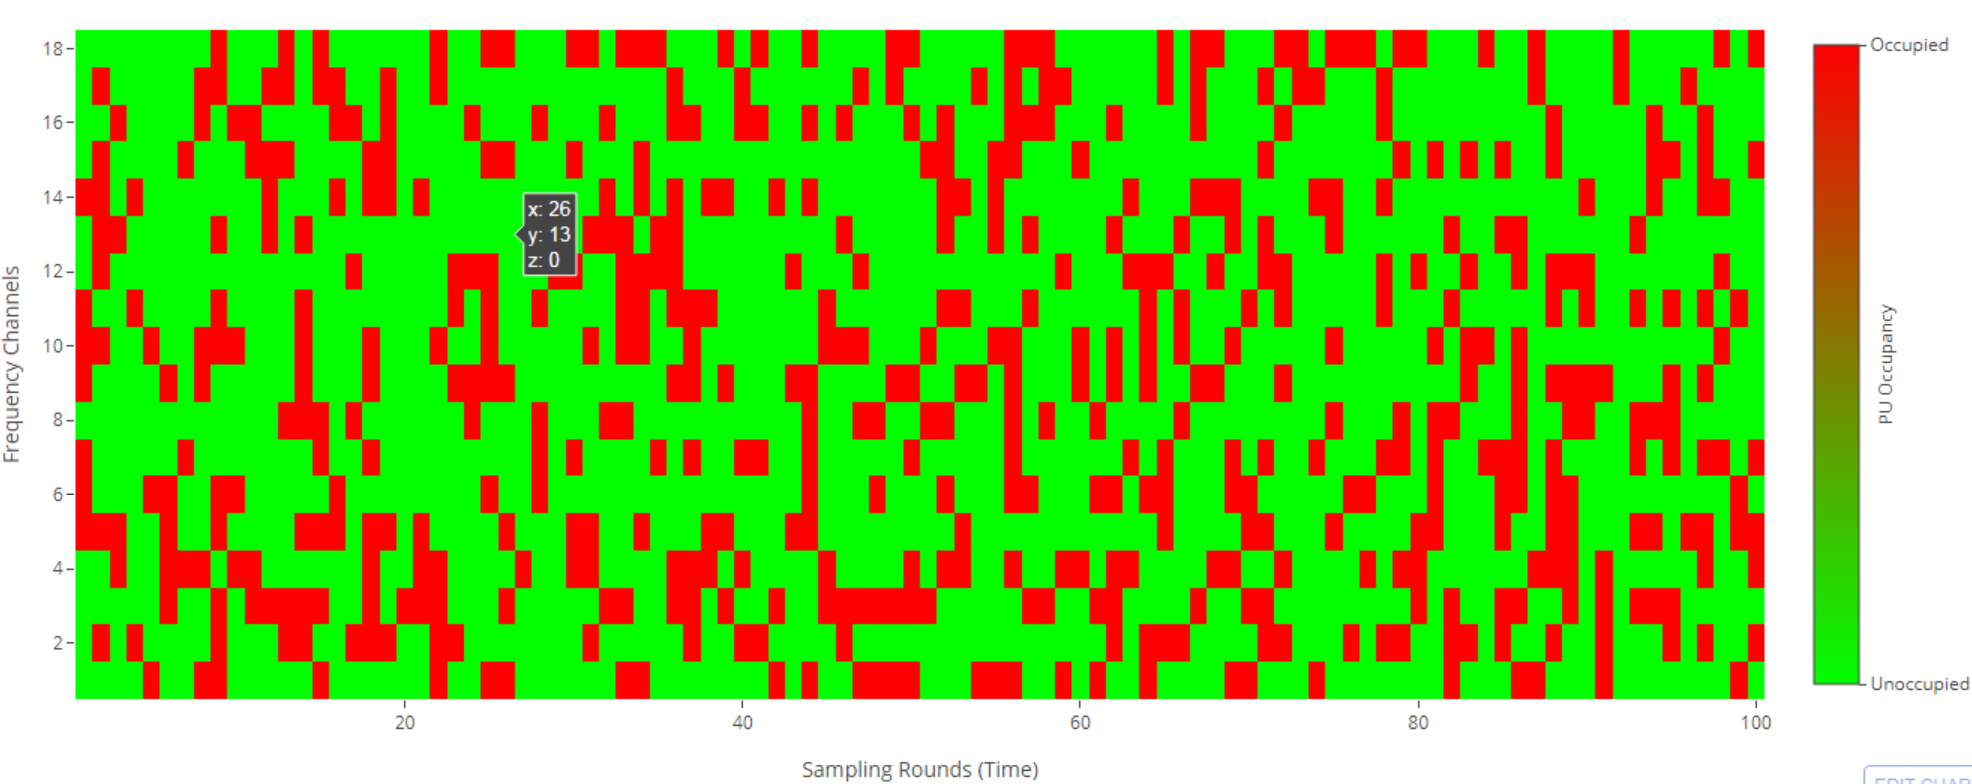
\includegraphics[width = 1.0\textwidth]{Independence_1.PNG}
    \caption{The time-frequency incumbent occupancy behavior assuming independence across both frequency and time}
    \label{fig:29}
\end{figure}
\end{frame}
\begin{frame}{Numerical Evaluations (2/7)}
    \begin{figure}
    \centering
    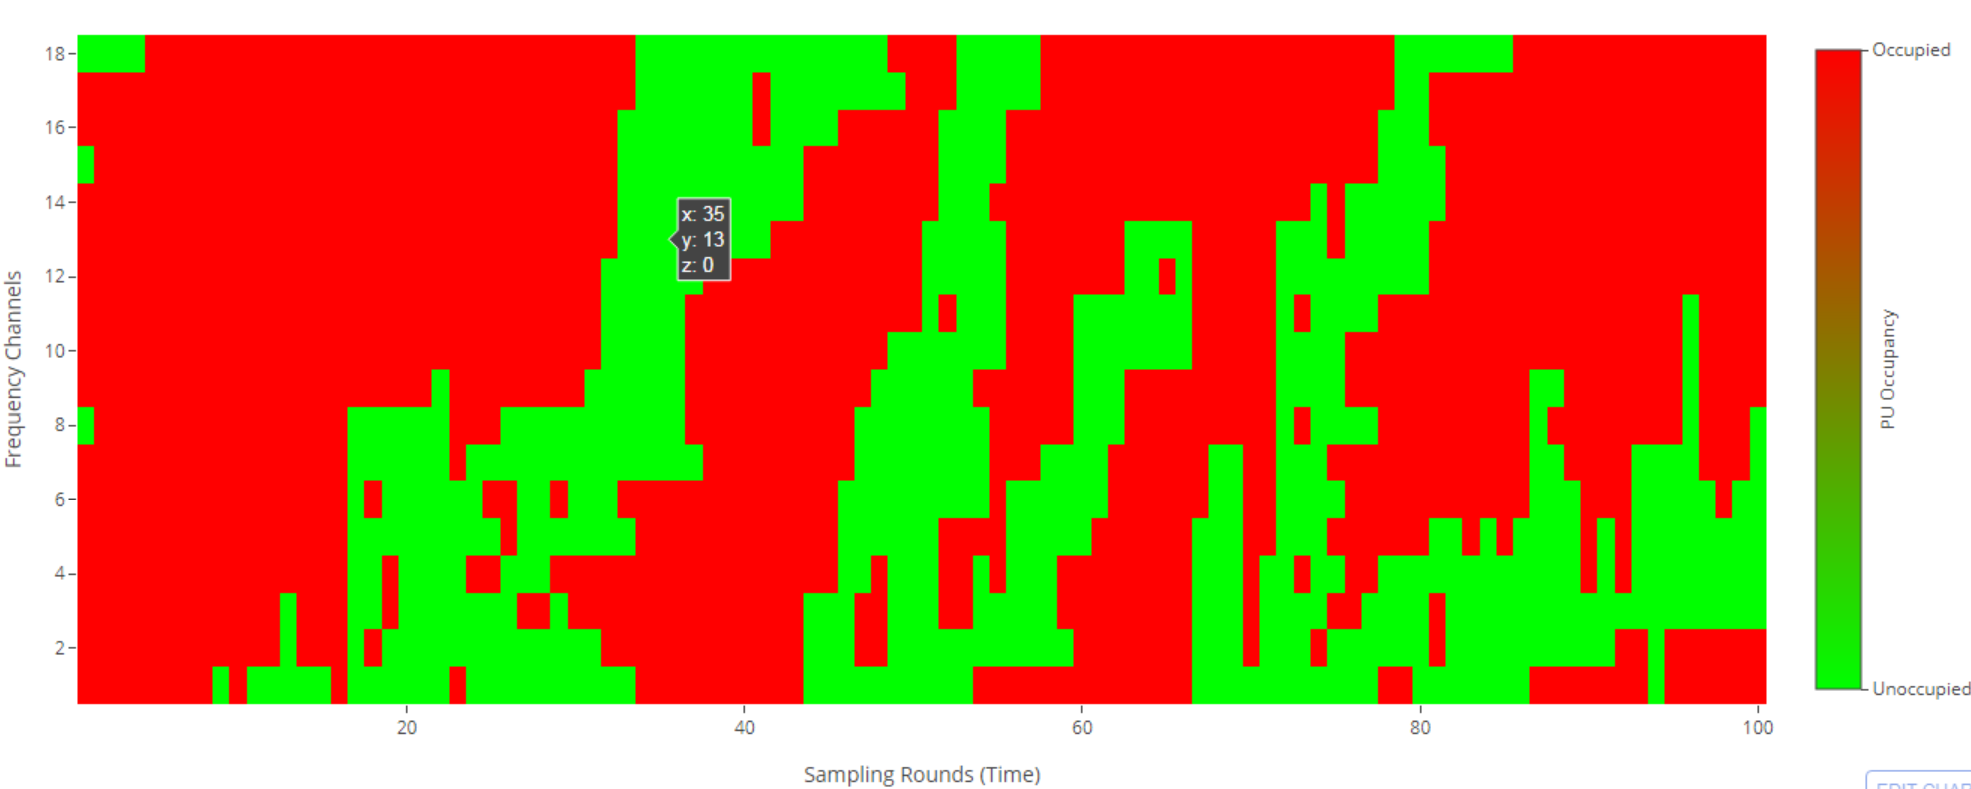
\includegraphics[width = 1.0\textwidth]{Space_Time_Corr_1.PNG}
    \caption{The time-frequency incumbent occupancy behavior assuming a Markovian correlation across both frequency and time}
    \label{fig:30}
\end{figure}
\end{frame}
\begin{frame}{Numerical Evaluations (3/7)}
    \begin{figure}
    \centering
    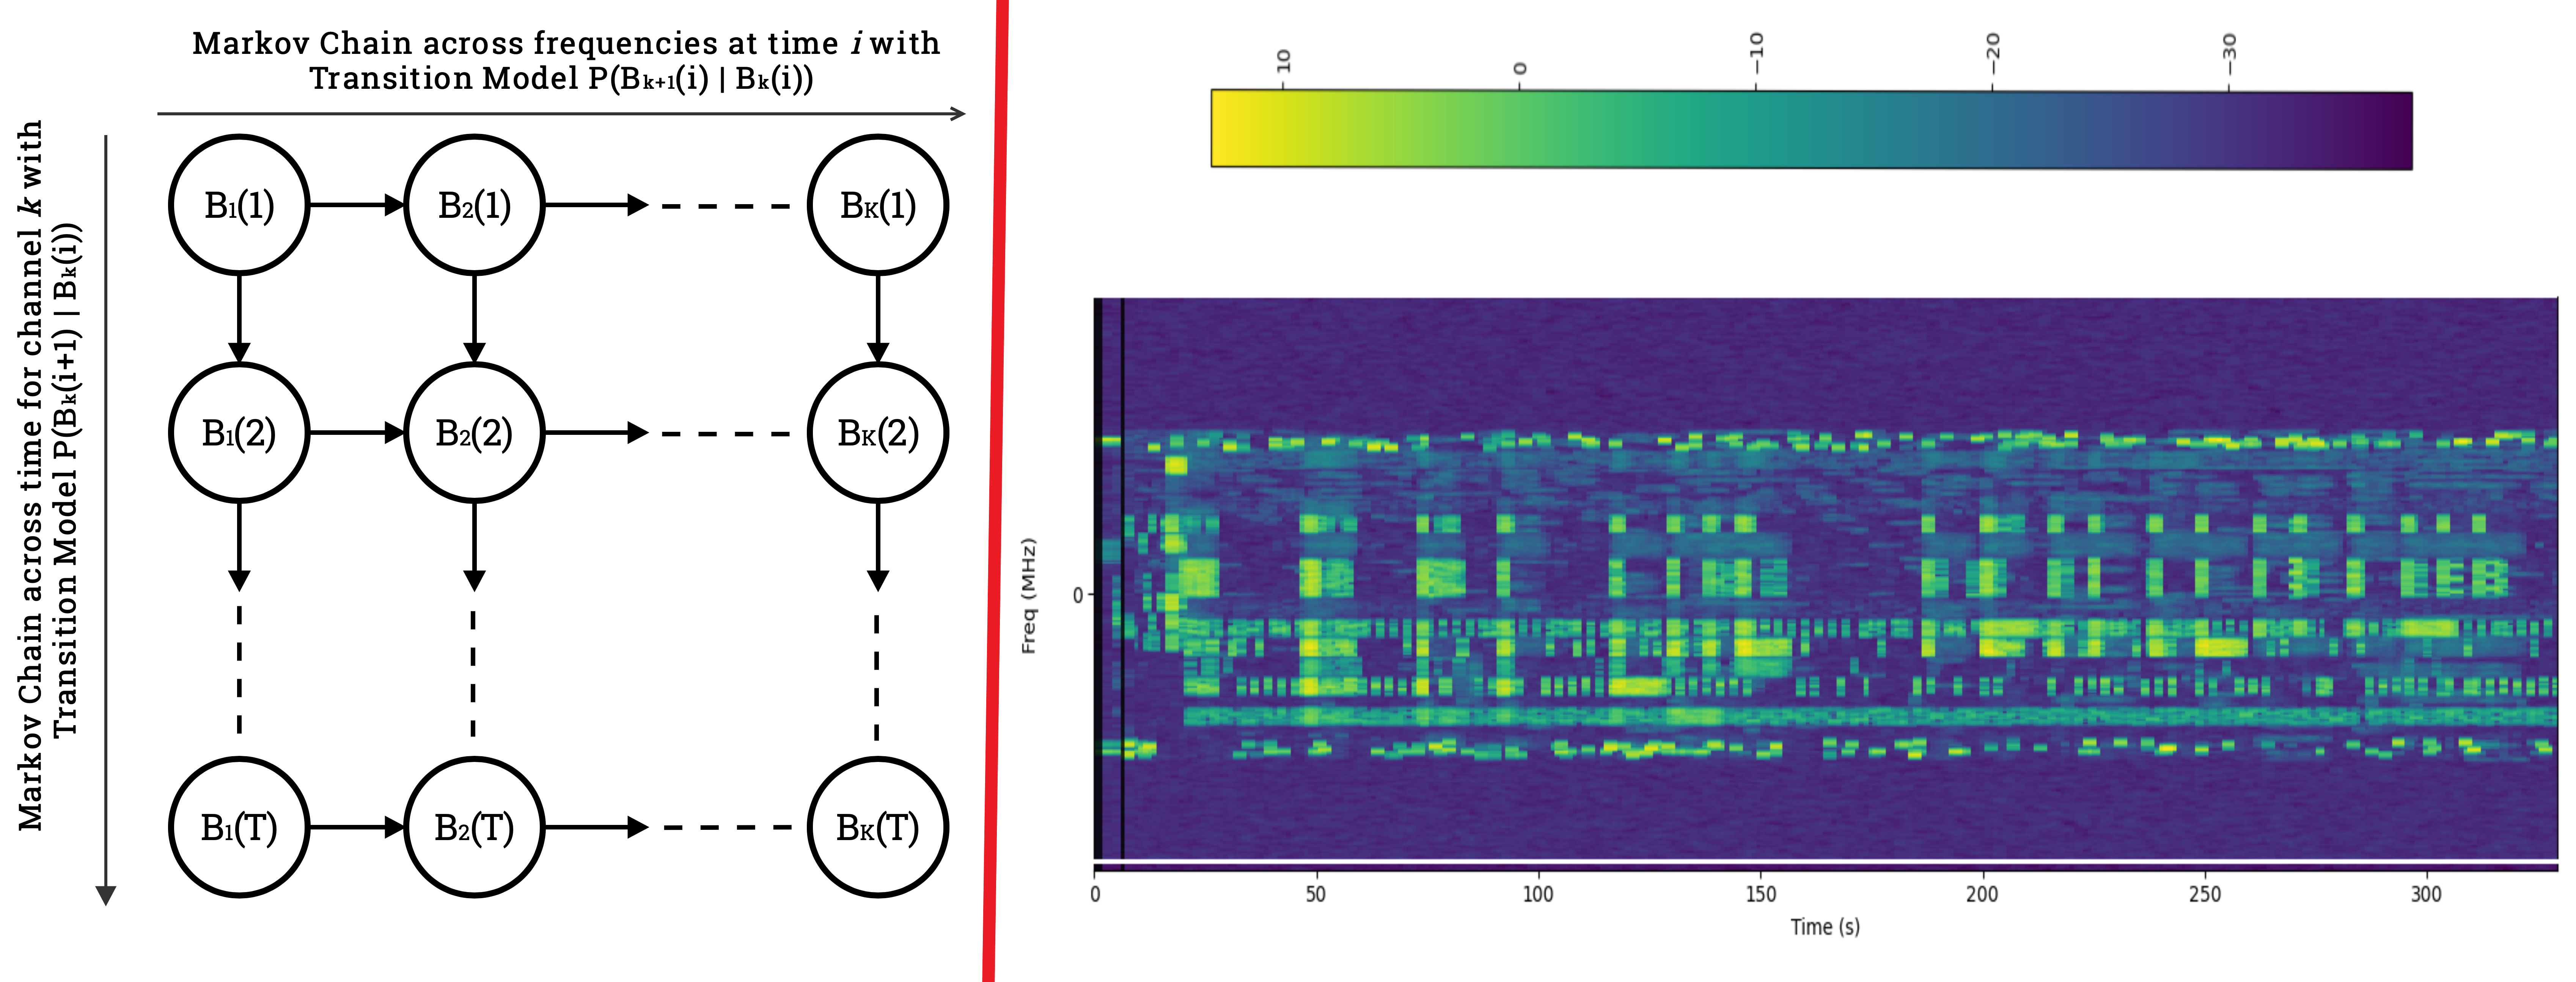
\includegraphics[width = 0.85\textwidth]{MarkovChainsVisualization.png}
    \caption{The time-frequency correlation structure of the incumbent occupancy behavior assumed in our simulations according to discussions in the ``PU Occupancy Model" section}
    \label{fig:31}
\end{figure}
\end{frame}
\begin{frame}{Numerical Evaluations (4/7)}
    \begin{figure}
    \centering
    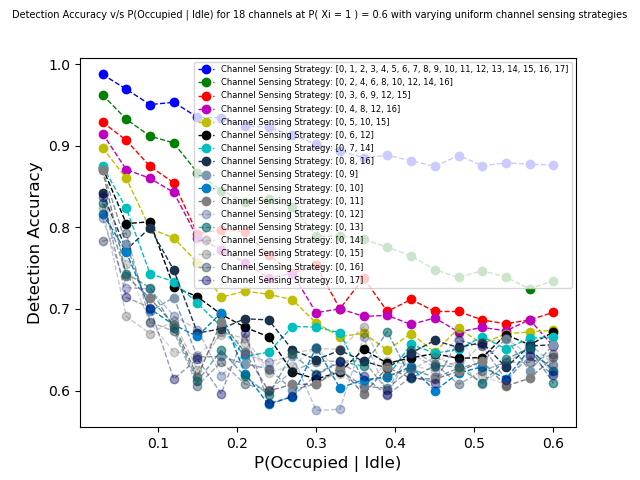
\includegraphics[width = 0.85\textwidth]{Uniform_Channel_Sensing.png}
    \caption{Single Markov chain across channels: Effect of channel sensing limitations, channel correlation, and sensing strategies on estimation/detection accuracy}
    \label{fig:32}
\end{figure}
\end{frame}
\begin{frame}{Numerical Evaluations (5/7)}
    \begin{figure}
    \centering
    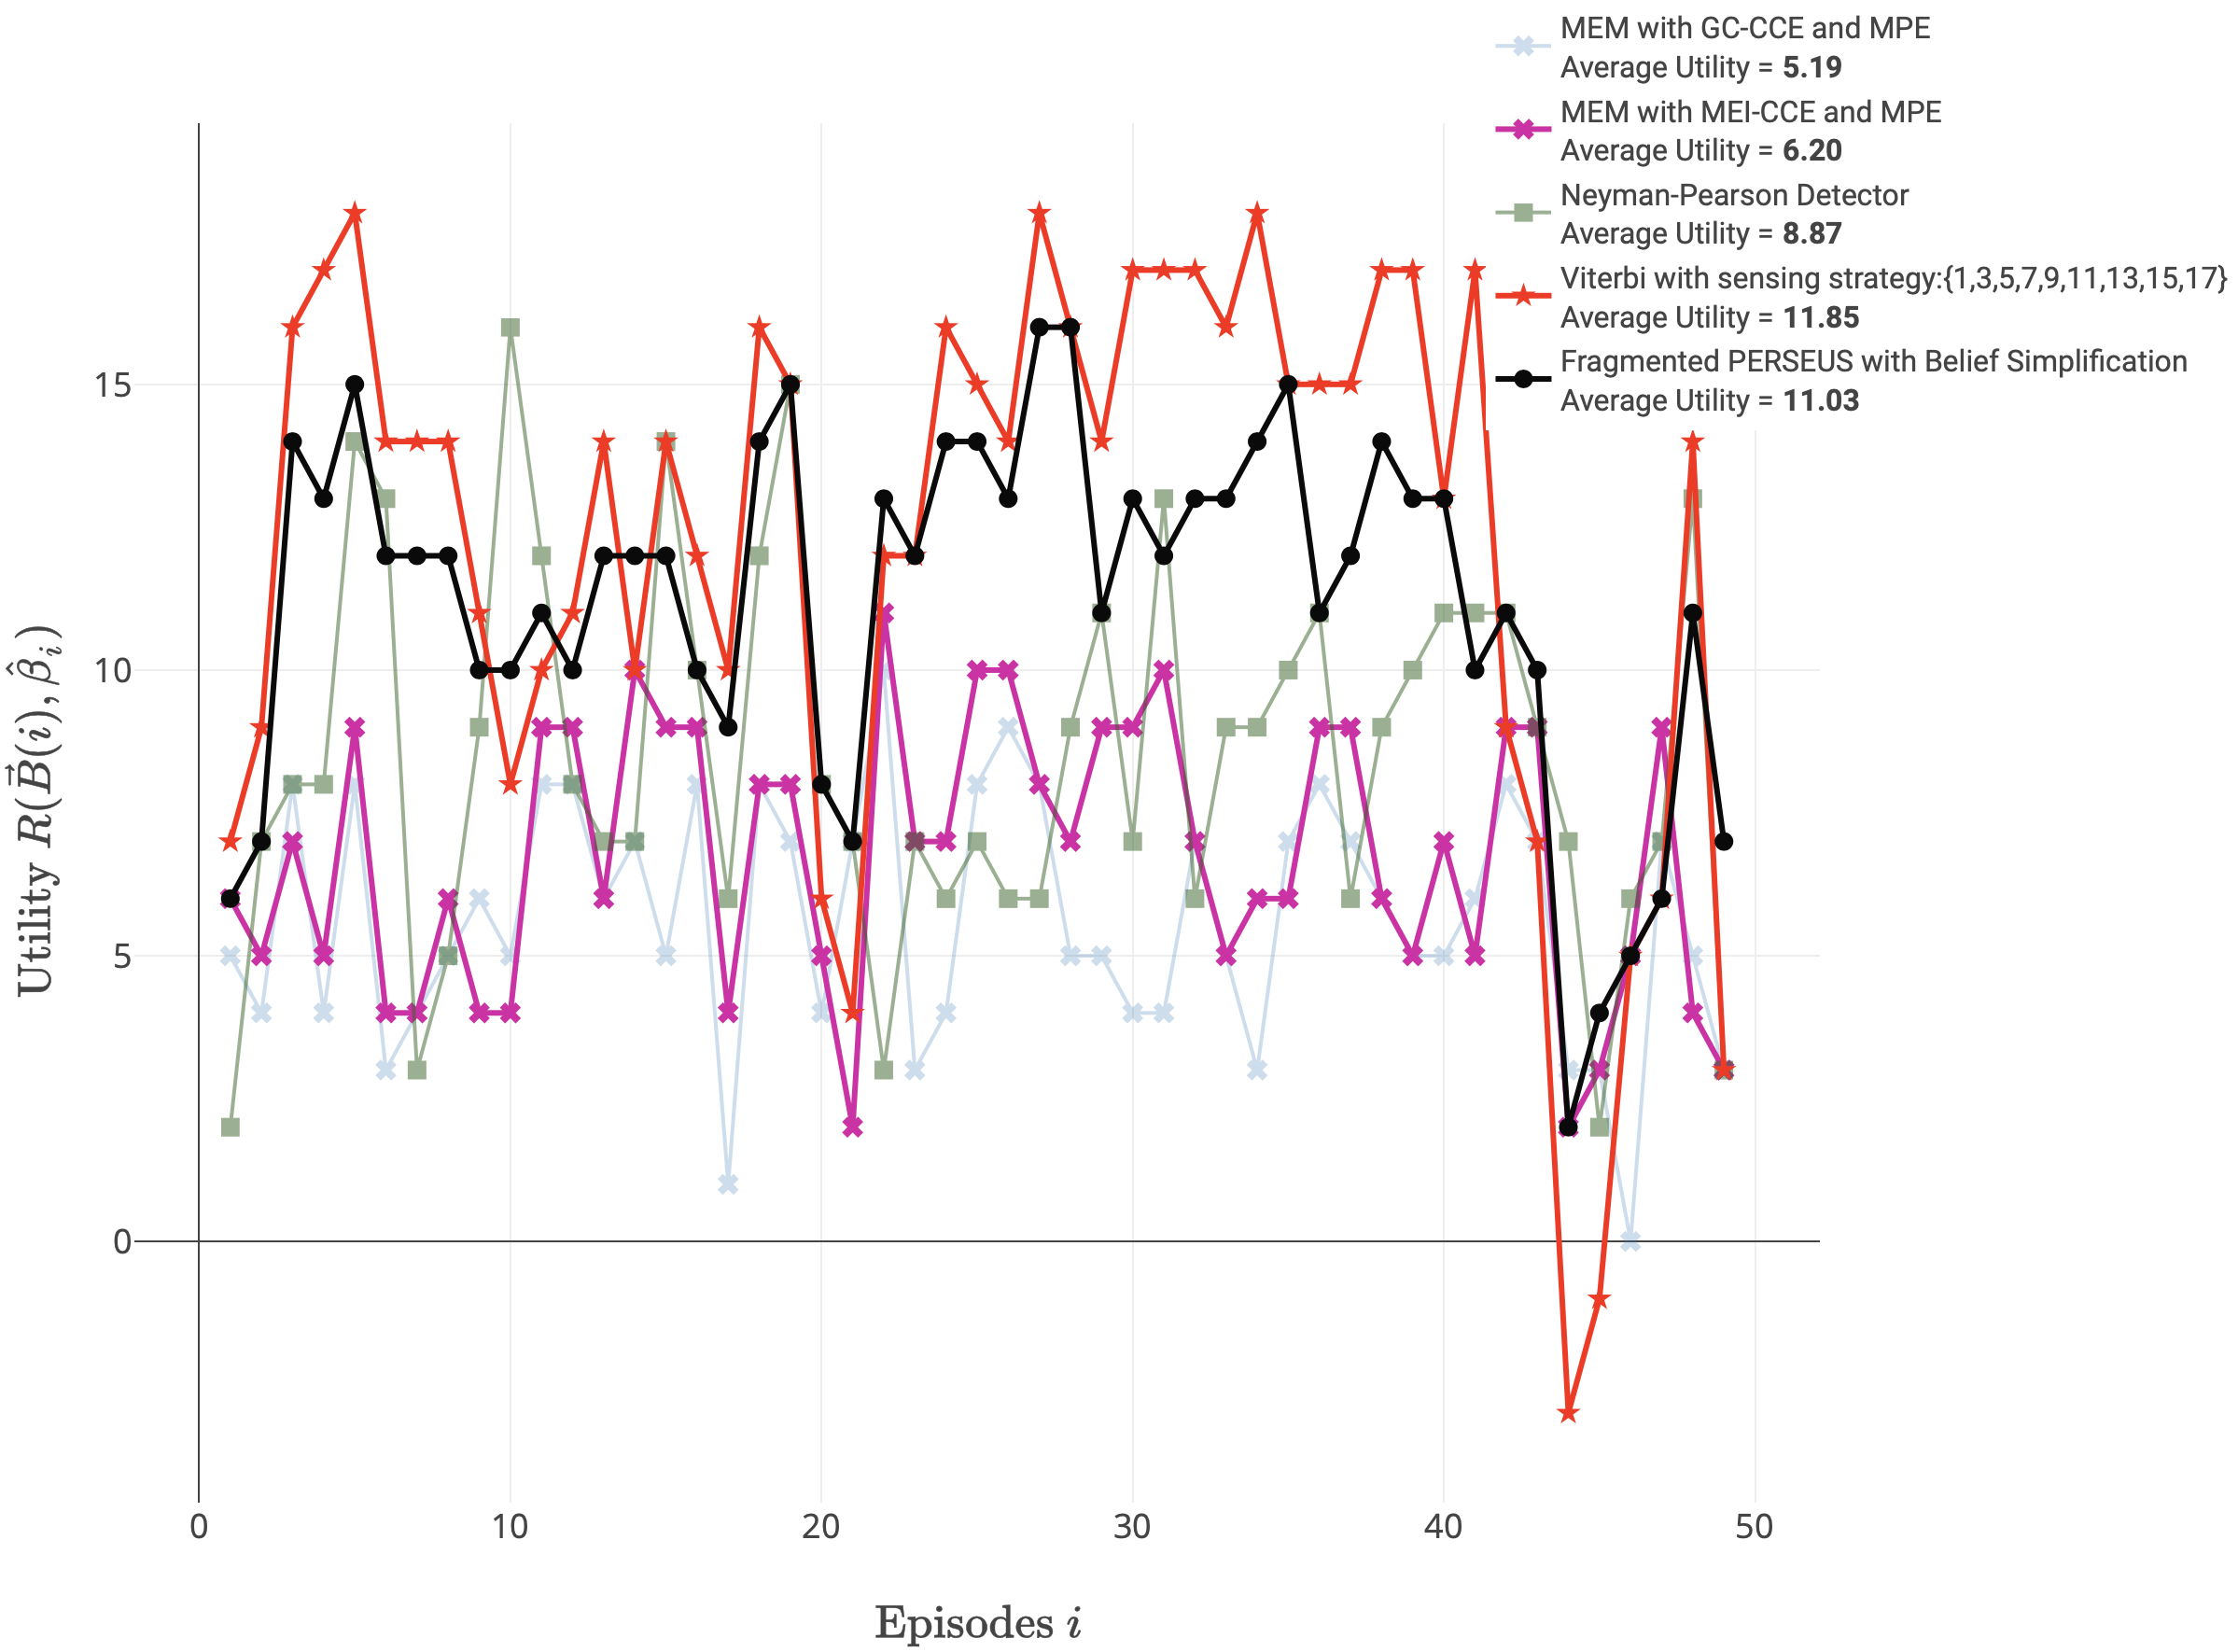
\includegraphics[width = 0.95\textwidth]{PerformanceEvaluation.png}
    \caption{The comparison of the utility obtained by our framework per time-slot against that obtained by other schemes in the state-of-the-art}
    \label{fig:33}
\end{figure}
\end{frame}
\begin{frame}{Numerical Evaluations (6/7)}
    \begin{figure}
    \centering
    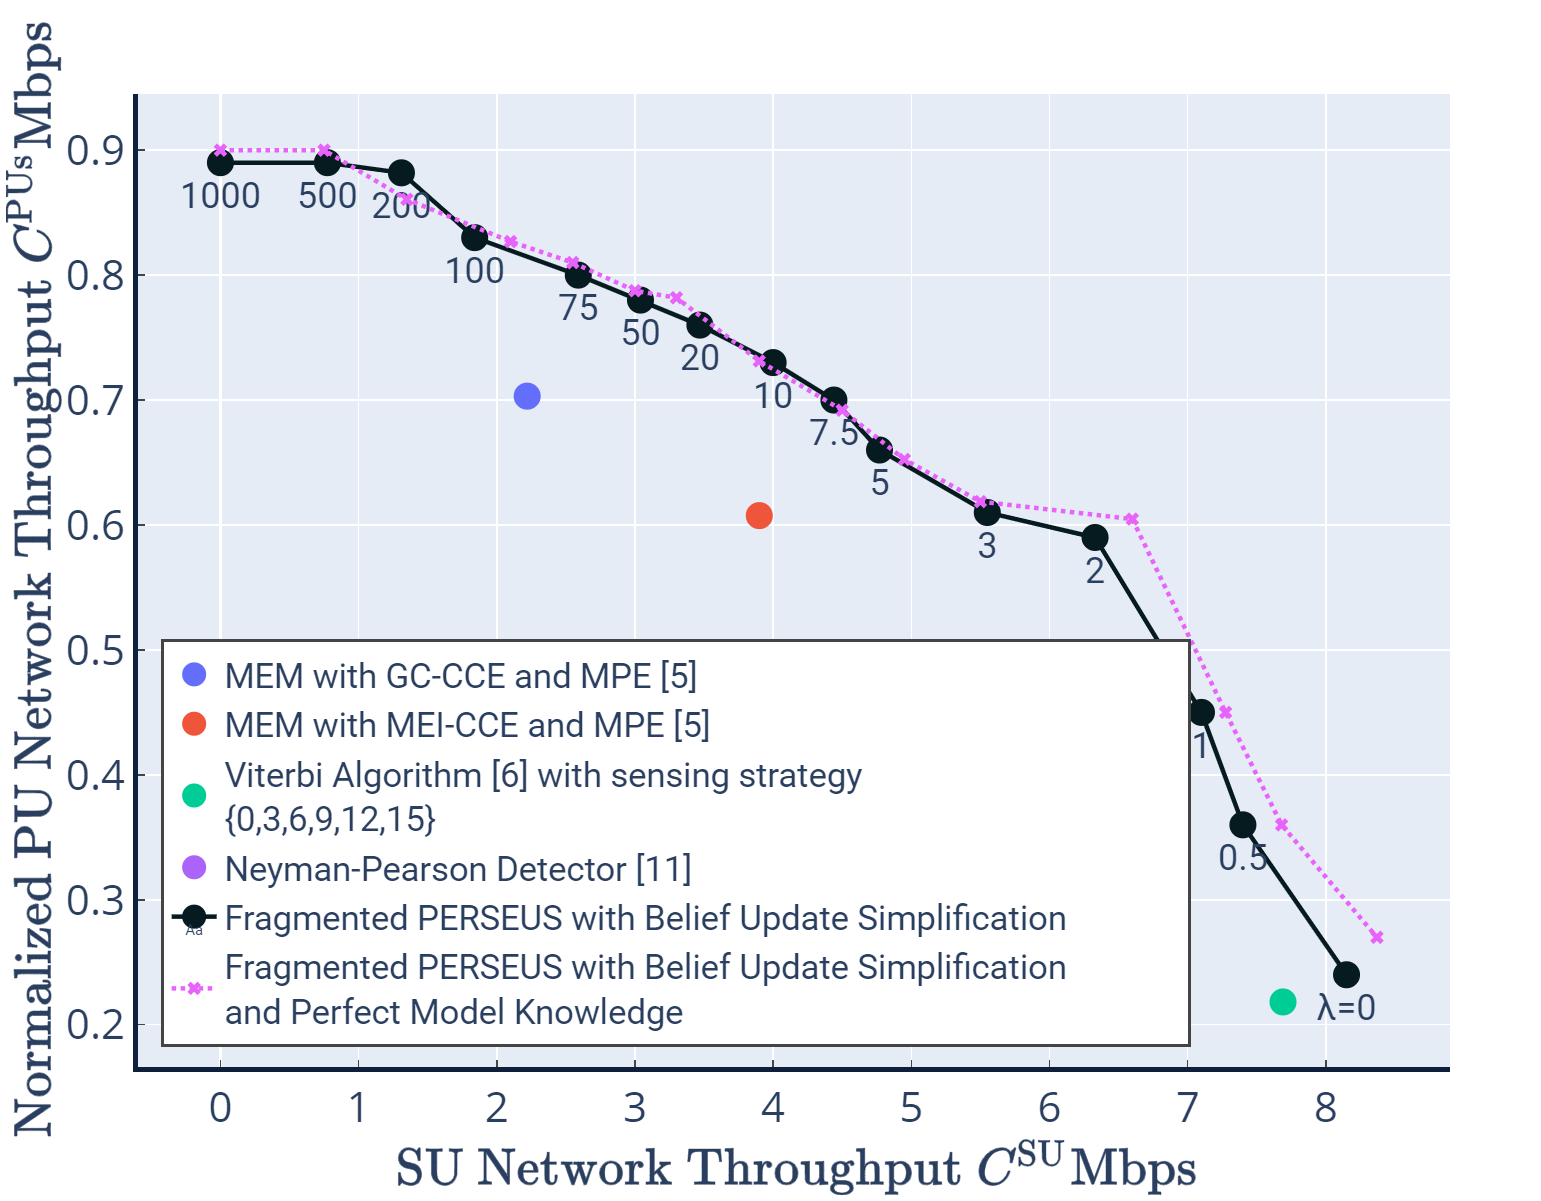
\includegraphics[width = 0.85\textwidth]{Final.PNG}
    \caption{Evaluation of $C^{\text{SU}}$ versus $C^{\text{PUs}}$ for different values of the penalty $\lambda$; comparison with state-of-the-art}
    \label{fig:34}
\end{figure}
\end{frame}
\begin{frame}{Numerical Evaluations (7/7)}
    \begin{figure}
    \centering
    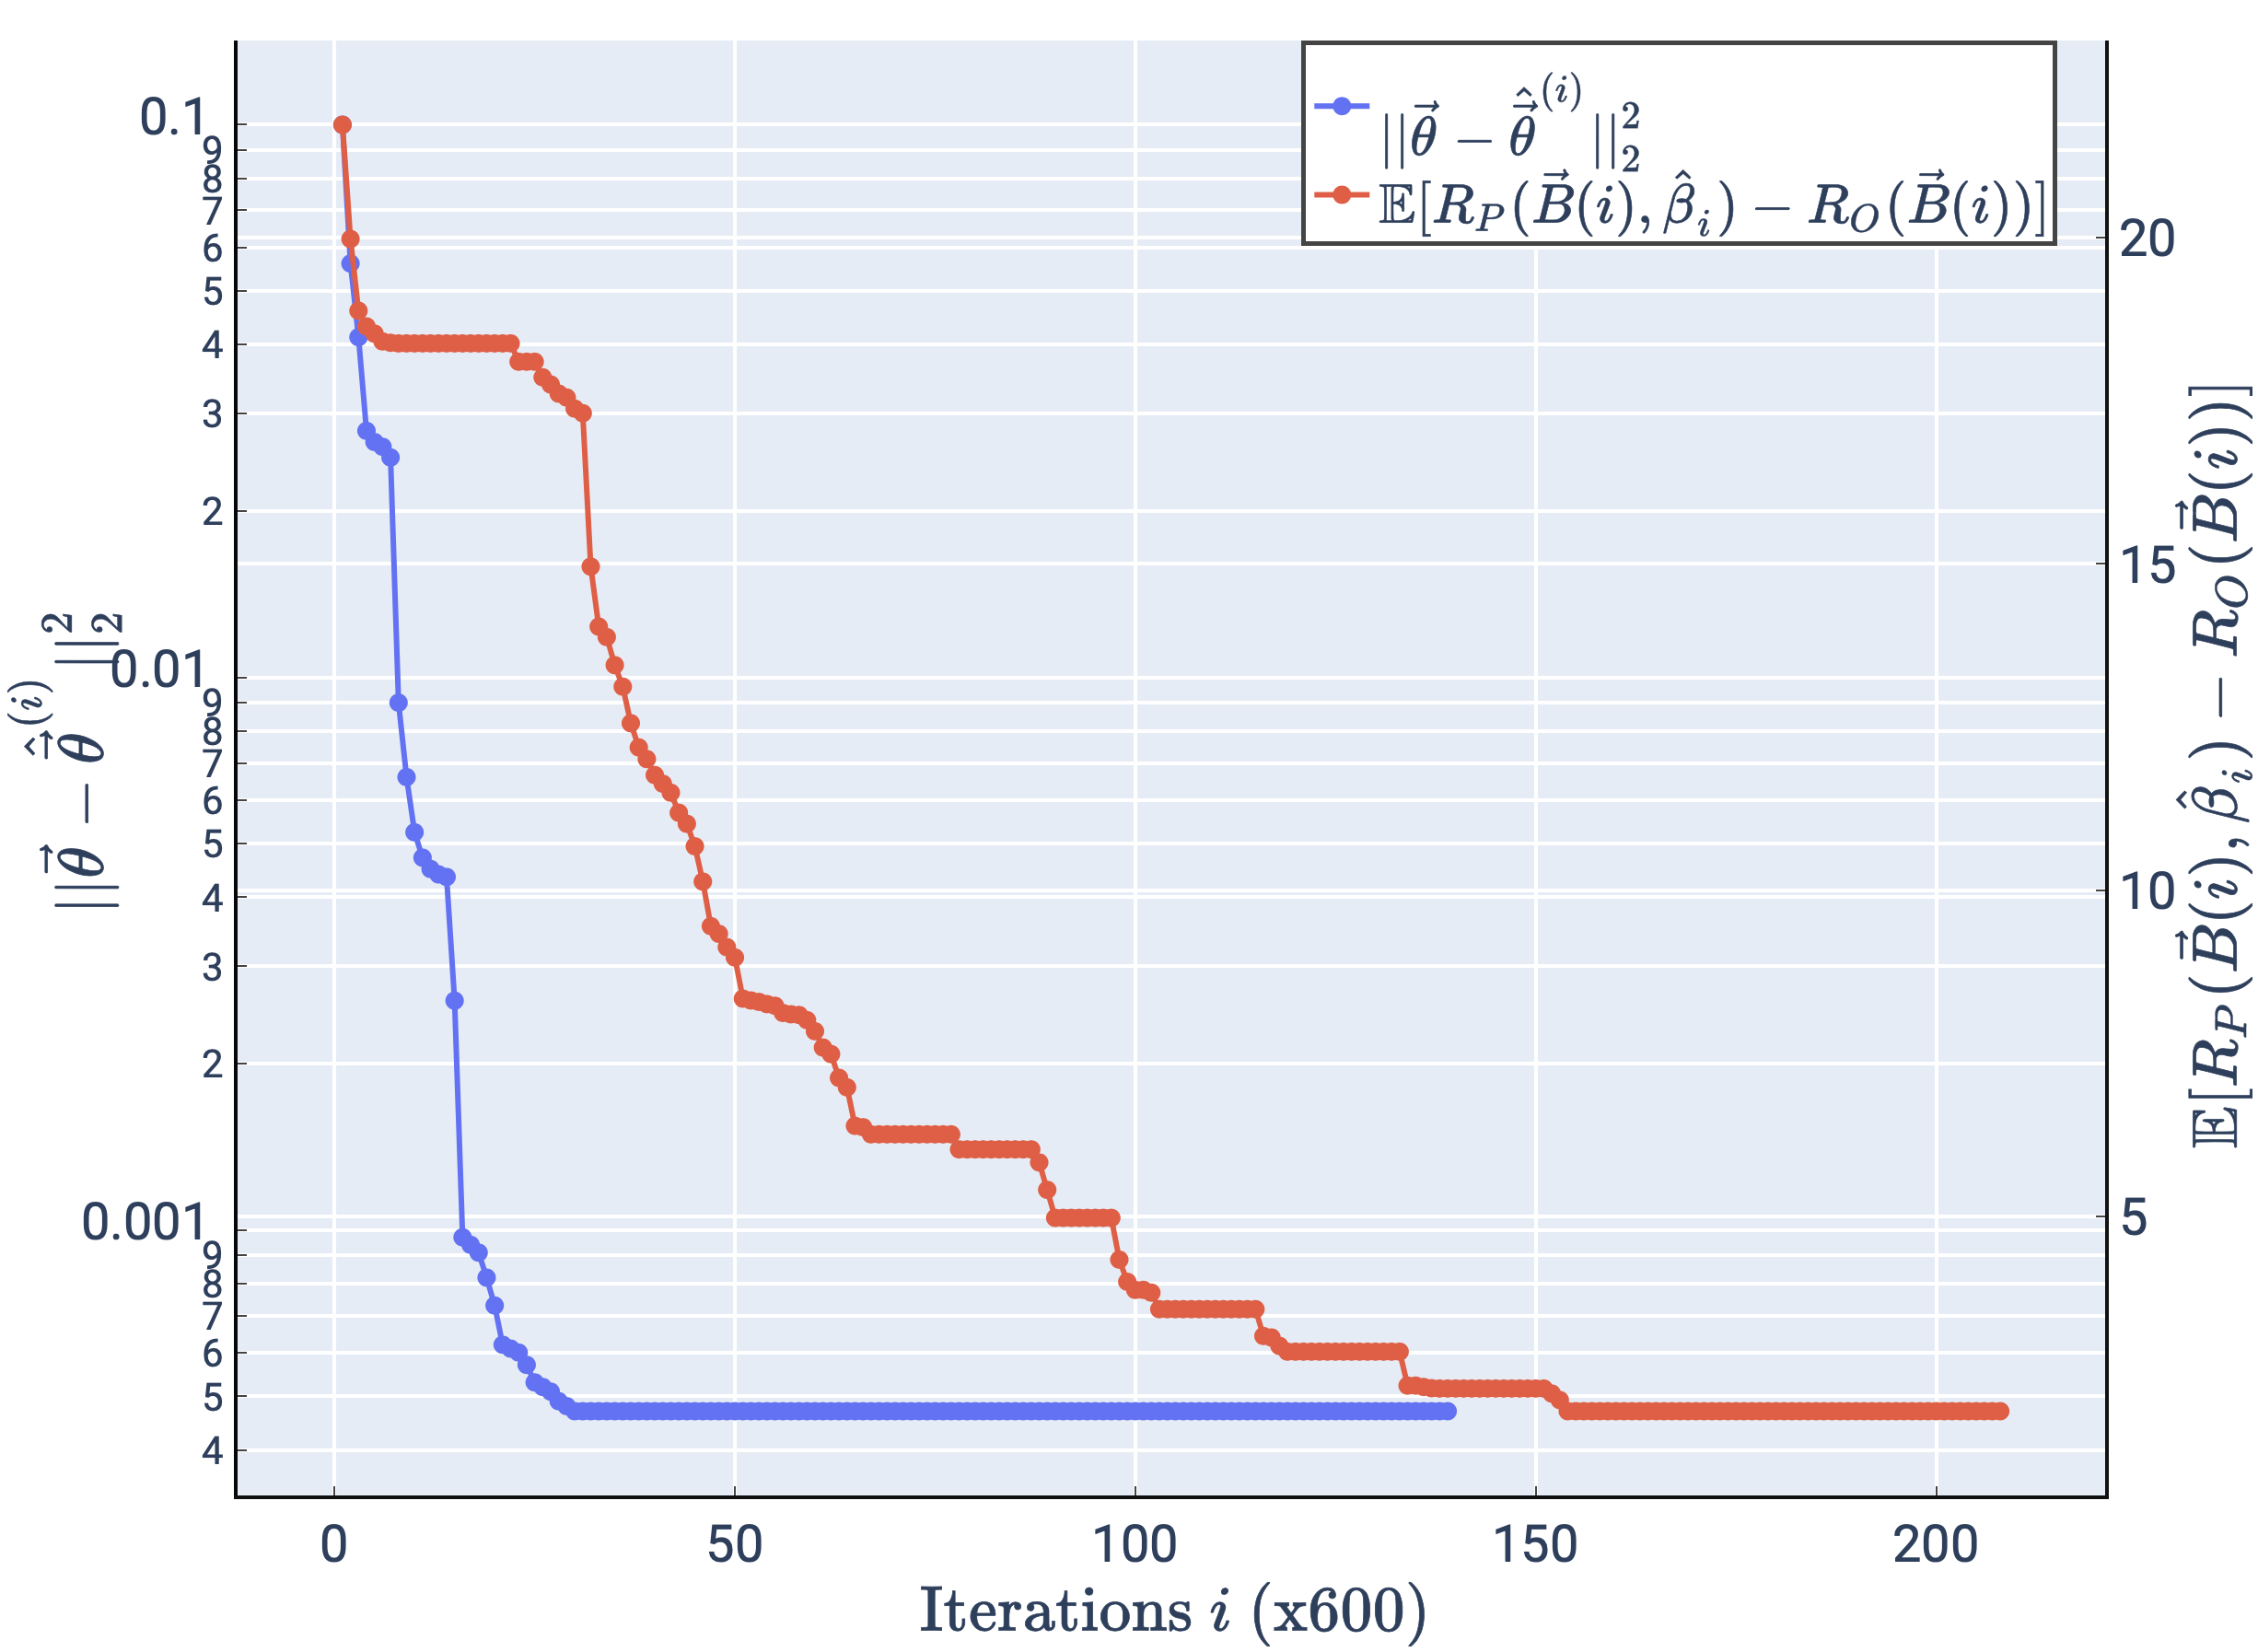
\includegraphics[width = 0.85\textwidth]{PerseusRegretConvergence_NormSquareErrorConvergence.png}
    \caption{Convergence of: MSE of the EM algorithm to estimate $\vec{\theta}$; and Loss of the fragmented PERSEUS algorithm with belief update simplification}
    \label{fig:35}
\end{figure}
\end{frame}
\begin{frame}{}
  \centering \Huge
  \emph{Implementation Analysis\\
        \LARGE{Optimal POMDP Policy on ESP$32$ Radios}}
\end{frame}
\begin{frame}{POMDP Access Policy Implementation}
    \scriptsize{\begin{itemize}
        \item $8$ ESP$32$\footnote{\tiny{Espressif, ``Espressif ESP32: A Different IoT Power and Performance", 2019}} radios, each embedded on a GCTronic e-puck2\footnote{\tiny{GCTronic, ``e-puck2 Specifications and General Wiki", 2020}} robot: $3$ PU source-sink pairs and $2$ SUs in a $6$ channel radio environment\texttt{-{}-}each SU capable of sensing and accessing only $1$ channel in a given time-slot
        \item Simulate the occupancy behavior of these $3$ PUs according to the Markovian time-frequency correlation structure discussed earlier, and export this time-slotted behavior to a database
        \item Simulate a single SU with a sensing limitation of $2$ and that which is capable of accessing $2$ channels per time-slot
        \item Learn the transition model of the environment and the corresponding optimal sensing policy on a PC, as discussed earlier
        \item Export the optimal sensing decisions in each of these time-slots to a database
        \item Establish peer-to-peer communication w.r.t the PUs in the network over $2.4$GHz WiFi: the source PU acts as an AP and its sink serves as a STA over this ad-hoc distributed WLAN\texttt{-{}-}the channel occupancy is dictated by the exported time-slotted occupancy database
        \item Based on the exported policy database, the SUs then sense the corresponding channels (split between the two), i.e., look for incumbent frames (BSSID checks), and access these channels for their flows if they are deemed to be idle
        \item Evaluate the time-slotted channel access success probability by collating results from each individual SU
    \end{itemize}}
\end{frame}
\begin{frame}{Channel Access Success Rate}
    \begin{figure}
    \centering
    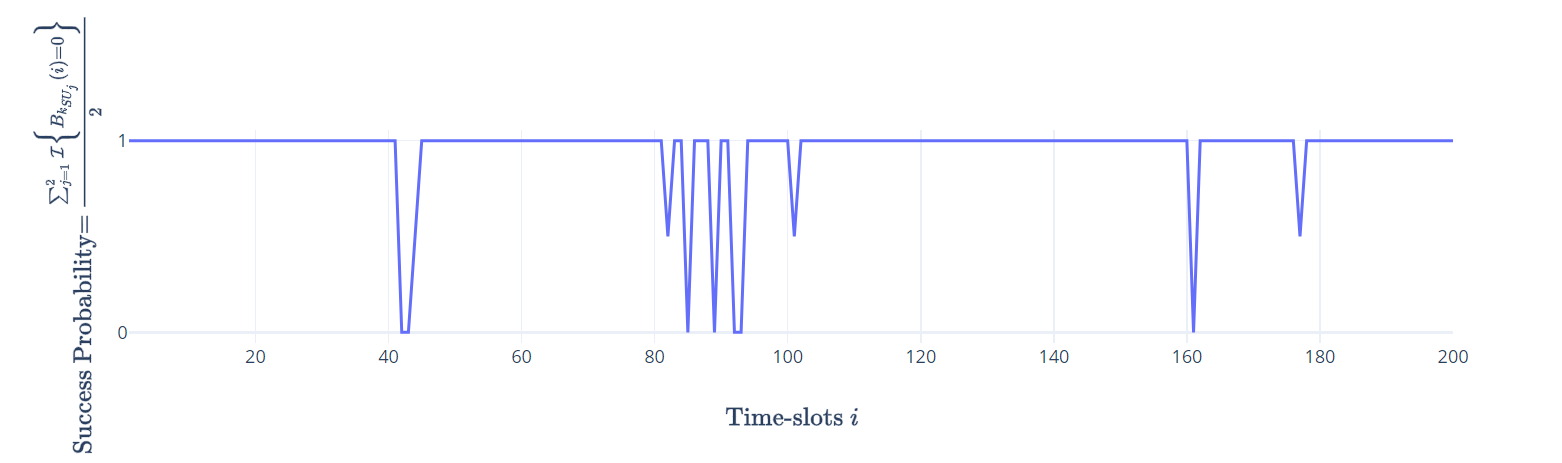
\includegraphics[width = 1.0\textwidth]{ESP32_Success_Probability.PNG}
    \caption{The time-slotted success probability of the cognitive radios (SUs) in this distributed ad-hoc network of ESP$32$ radios over $2.4$GHz WiFi channels}
    \label{fig:36}
\end{figure}
\end{frame}
\begin{frame}{}
  \centering \Huge
  \emph{Q\&A}
\end{frame}
\begin{frame}{}
  \centering \Huge
  \emph{Thank you}
\end{frame}
\end{document}